\documentclass[lettersize,journal]{IEEEtran}

\usepackage{amsmath,amsfonts,amssymb}

\usepackage{algorithmic}

\usepackage{algorithm}

\usepackage{array}

\usepackage[caption=false,font=normalsize,labelfont=sf,textfont=sf]{subfig}

\usepackage{textcomp}

\usepackage{stfloats}

\usepackage{url}

\usepackage{verbatim}

\usepackage{graphicx}

\usepackage{cite}

\usepackage{booktabs}

\usepackage{multirow}

\usepackage{bm}

\usepackage{color}

\usepackage{float}

\usepackage{flafter}

\usepackage{makecell}

\usepackage{setspace}

\usepackage[hidelinks,unicode]{hyperref}
\renewcommand{\algorithmicrequire}{\textbf{Input:}}
\renewcommand{\algorithmicensure}{\textbf{Output:}}

\hyphenation{op-tical net-works semi-conduc-tor IEEE-Xplore}

\begin{document}

\title{Multi-Goal Traversal Planning in Cluttered Environments via Improved A* and MMAS-VND-CL}

\author{Author Name~\IEEEmembership{Member,~IEEE}%
\thanks{Author affiliation and correspondence information to be supplied.}%
\thanks{Manuscript received 2026; revised 2026.}}

\markboth{Journal Preprint}%
{Multi-Goal Traversal Planning via Improved A* and MMAS-VND-CL}

\maketitle

\begin{abstract}

In modern development, exploring technologies involving multi-goal traversal path planning, such as unmanned shuttle services and logistics delivery, is of great importance. Among the related technologies, grid-based map modeling can significantly simplify the path-planning process, especially in complex environments with a large number of intermediate nodes. To address the multi-goal traversal problem in grid-based obstacle environments, this paper proposes a two-layer collaborative planning framework that integrates an improved A* with Max-Min Ant System-Variable Neighborhood Descent-Candidate List (MMAS-VND-CL). The framework combines Jump Point Search (JPS)-based global pathfinding with open traveling salesman combinatorial ordering, achieving a unified solution at the geometric and ordering layers. The geometric layer employs an improved A* that combines safety-aware path simplification with arc-length-parameterized spline smoothing to smoothly generate collision-free continuous paths between point pairs and to construct the traveling-salesman cost matrix; the ordering layer proposes the MMAS-VND-CL algorithm, which solves the open traveling salesman problem with fixed start and end points by the virtual-node method. A key feature of MMAS-VND-CL is the candidate-list-accelerated Variable Neighborhood Descent (VND) local search, which confines neighborhood evaluation to the nearest neighbors and thus refines tours efficiently even at large target scales; meanwhile, the algorithm integrates the pheromone bounds of the Max-Min Ant System to maintain search diversity, an Ant Colony System-style pseudo-random transition to balance exploration and exploitation, and an S-shaped progressive schedule to control the timing of local-search effort. To evaluate the effectiveness of the proposed framework, the improved A* is performance-tested on three grid maps with different obstacle morphologies, and parameter sensitivity analysis, ablation experiments, and solver comparison experiments are conducted for MMAS-VND-CL. The results show that the improved A* performs better: compared with the traditional A* algorithm, it reduces the planned path length on Map~3 by 5.3\% and the planning time by 75.9\%. In the comparative experiments on MMAS-VND-CL, it reduces the average path length on Map~1 by 10.0\% and the running time by 57.4\% compared with traditional ACO.

\end{abstract}

\begin{IEEEkeywords}

multi-goal traversal, path planning, ant colony optimization, open traveling salesman problem

\end{IEEEkeywords}

\section{Introduction}

Multi-goal traversal path planning is a fundamental problem in autonomous mobile robotics, with broad applications in autonomous shuttle services, logistics and warehouse management, infrastructure inspection, and search-and-rescue operations \textcolor{blue}{\cite{ref1,ref2,ref33,ref37,ref38}}. In tasks such as passenger pickup and drop-off, equipment inspection, and item delivery, a robot must depart from a designated start location, visit a sequence of intermediate target points, and finally reach a designated goal. The planner must address two mutually coupled subproblems: finding collision-free paths between consecutive point pairs in cluttered environments, which is a geometric problem requiring reasoning about obstacle geometry and path continuity in physical space; and determining the optimal visitation order of the intermediate target points, which is a combinatorial optimization problem analogous to classical NP-hard problems such as the traveling salesman problem (TSP). The two subproblems interact: the traversal cost between any two points depends on the obstacles lying between them, while the optimal visitation order in turn depends on these pairwise traversal costs.

In general, existing multi-goal navigation methods tend to handle only one of the two subproblems in isolation. A large body of TSP research assumes that pairwise costs are given by Euclidean distance or a known distance matrix \textcolor{blue}{\cite{ref4,ref36}}, overlooking the fact that, in obstacle-rich environments, the shortest collision-free path between two points can be far longer than their straight-line distance \textcolor{blue}{\cite{ref39}}. On the other hand, mature path-planning algorithms such as A*, Dijkstra, and rapidly-exploring random trees (RRT) and their variants can efficiently compute optimal or near-optimal collision-free paths between point pairs on grid maps, but these planners do not optimize the visitation order of multiple goals \textcolor{blue}{\cite{ref5,ref6,ref7}}. A few studies have explored obstacle-aware TSP variants under specific geometric assumptions (e.g., TSP with obstacles, Dubins TSP); however, a general framework that integrates a grid-based global planner with a high-performance TSP solver for multi-goal traversal in cluttered environments is still lacking.

To address these constraints and fully exploit the strengths of both algorithm families, this paper proposes a collaborative optimization framework for multi-goal traversal path planning in cluttered environments. The framework consists of two algorithmic layers connected by a precomputed cost matrix. The first layer is an improved A* global planner based on Jump Point Search (JPS), which exploits grid symmetry to skip redundant node expansions and expands only jump points, thereby greatly reducing the search-tree size; this planner is combined with a safety-aware path simplification procedure and an arc-length parameterized cubic spline smoothing pipeline. The second layer is an improved ant colony optimization (ACO) solver for the open TSP. It converts the open TSP into a standard closed-loop TSP by means of a virtual (dummy) node, thus fully exploiting closed-loop TSP search operators. The solver integrates Max--Min Ant System (MMAS) pheromone management, an Ant Colony System (ACS)-style pseudo-random transition rule, a Variable Neighborhood Descent (VND) local search engine accelerated by a $k$-nearest-neighbor candidate list, and a sigmoid-based progressive local-search schedule with an adaptive stopping criterion.

To tackle the above issues, this paper develops a two-layer planning framework comprising pairwise path search and visitation-order optimization. The former generates feasible paths according to the obstacle layout and computes the corresponding costs; the latter takes this cost matrix as input to determine the visitation order of the targets. On this basis, the path-processing pipeline and the ant-colony ordering solver are improved, respectively. The main contributions are as follows.

\begin{enumerate}

\item A hierarchical solution procedure for multi-goal traversal with fixed start and goal. The lengths of continuous trajectories of obstacle-constrained pairwise paths serve as traversal costs between targets, yielding a cost matrix that links geometric path planning and visitation-order optimization and thereby mitigating the neglect of obstacle-detour costs incurred by Euclidean-distance-based ordering.

\item An improved A* path-planning and post-processing pipeline based on JPS. Incorporating tie-breaking, search-failure fallback, safety-distance-aware path simplification, and arc-length parameterized cubic spline smoothing, the pipeline reduces node expansions while producing continuous paths for cost computation; its planning efficiency and path length are analyzed through grid-map experiments.

\item An MMAS-VND-CL visitation-order solver. A virtual node handles the fixed-endpoint constraint of the open TSP; MMAS pheromone bounds, ACS-style pseudo-random transition, candidate-list-accelerated VND, sigmoid scheduling, and an adaptive stopping criterion are integrated. Parameter-sensitivity and ablation experiments analyze the effects of individual components on solution quality, stability, and runtime.

\end{enumerate}

The remainder of this paper is organized as follows. Section~\textcolor{blue}{\ref{sec:related}} reviews related work on global path planning, TSP metaheuristics, and multi-goal traversal with obstacles; Section~\textcolor{blue}{\ref{sec:form}} formalizes the problem; Section~\textcolor{blue}{\ref{sec:method}} details the methodology, including the improved A* planner, the path post-processing pipeline, the improved ACO solver, and the collaborative optimization framework; Section~\textcolor{blue}{\ref{sec:exp}} reports experimental results along four evaluation dimensions: global path-planning comparison, parameter sensitivity analysis, ablation studies, and multi-goal traversal comparison among different TSP solvers; Section~\textcolor{blue}{\ref{sec:concl}} concludes the paper and outlines future work.



\section{Related Work}
\label{sec:related}

\subsection{Existing Path Search Methods and Their Limitations}

Global path planning aims to find a collision-free path between two points in a known static environment, and classical graph-search algorithms constitute the mainstream approach to grid-based planning\textcolor{blue}{\cite{ref33,ref34,ref35}}. Dijkstra's algorithm expands uniformly and is therefore inefficient on large maps\textcolor{blue}{\cite{ref6}}; A* guides the search with a heuristic and preserves optimality whenever $h(n)$ is admissible\textcolor{blue}{\cite{ref5}}, yet a fixed heuristic weight entails a trade-off: a weight of 1 expands too many nodes, whereas a larger weight sacrifices optimality\textcolor{blue}{\cite{ref8}}. Variants such as weighted A* and anytime repairing A* apply a uniform weight throughout the search\textcolor{blue}{\cite{ref8,ref10}}, whereas a practically useful weight intuitively depends on the distance to the goal. Jump point search (JPS) exploits grid symmetry to expand only jump points, thereby greatly compressing the search tree\textcolor{blue}{\cite{ref11,ref12,ref44}}; recent variants further introduce bidirectional search and any-angle refinement\textcolor{blue}{\cite{ref13,ref14,ref15}}, and the improved A* developed in this paper is built on this principle. Sampling-based planners such as RRT\textcolor{blue}{\cite{ref7}} and PRM offer probabilistic completeness and perform well in high-dimensional configuration spaces, but the solution paths they produce in grid environments are typically longer and less consistent.

Post-processing of grid paths is a well-established practice, including collinearity or line-of-sight pruning\textcolor{blue}{\cite{ref16}} and smoothing methods such as cubic splines, B-splines, and clothoids\textcolor{blue}{\cite{ref17,ref18,ref41}}. However, pruning and smoothing are usually treated as independent a posteriori steps and are not incorporated into the computation of the multi-goal cost. Using the continuous path length obtained after post-processing to guide the combinatorial optimization is a distinguishing feature of the proposed framework.

\subsection{Existing Visit-Order Optimization Methods and Their Deficiencies}

The traveling salesman problem is among the most extensively studied problems in combinatorial optimization\textcolor{blue}{\cite{ref4,ref36}}. Exact algorithms are typically applicable only to small instances; larger instances usually resort to metaheuristics such as genetic algorithms\textcolor{blue}{\cite{ref19}} and ant colony optimization\textcolor{blue}{\cite{ref21,ref42}}. The pseudo-random proportional transition rule of the ant colony system (ACS)\textcolor{blue}{\cite{ref22}} and the explicit pheromone lower and upper bounds of the max--min ant colony system (MMAS)\textcolor{blue}{\cite{ref23}} improve convergence speed and search stability, respectively; the ordering solver adopted in this paper builds on both as modular components.

For the problem addressed in this paper, existing ordering methods suffer from two deficiencies. First, mainstream solvers assume by default that the pairwise cost is the Euclidean distance or a known distance matrix, whereas in obstacle environments the true traversal cost is determined by obstacle-avoidance paths. Second, embedding local search such as 2-opt and variable neighborhood descent (VND) into ant colony algorithms can substantially improve solution quality\textcolor{blue}{\cite{ref24,ref25,ref43}}, yet VND evaluates $O(K^2)$ candidate moves per operator and becomes a bottleneck when $K > 100$; candidate-list techniques can mitigate this cost by restricting neighborhood evaluation to the nearest neighbors\textcolor{blue}{\cite{ref26}}. Moreover, gradual scheduling of local search has received limited attention: most implementations apply local search to a fixed fraction of ants throughout the entire run, whereas recent ant colony variants focus mainly on parallelization, niching, and sustainability mechanisms\textcolor{blue}{\cite{ref27,ref28,ref29,ref30}}. To address these deficiencies, this paper incorporates obstacle cost through safety-aware arc-length pricing, accelerates VND with candidate lists (Section~\textcolor{blue}{\ref{subsec:vnd}}) to reduce the local-search complexity to $O(K \cdot k)$, and schedules the timing of local-search effort with a sigmoid scheme (Section~\textcolor{blue}{\ref{subsec:sigmoid}}).

\subsection{Combining the Two Method Families Under Obstacle Constraints}

The intersection of path planning and traveling-salesman optimization has been explored under various names\textcolor{blue}{\cite{ref4,ref36}}. Under continuous planar polygonal obstacles, pairwise traversal costs depend on obstacle-avoidance geometry rather than on the Euclidean metric\textcolor{blue}{\cite{ref39}}; Dubins variants account for minimum turning-radius constraints, and neighborhood or close-enough variants generalize targets from points to regions\textcolor{blue}{\cite{ref40}}. These formulations rely on continuous geometric representations and assume specific obstacle shapes, and hence are difficult to apply directly to grid navigation in which obstacles are represented by arbitrary occupancy patterns.

Two-layer architectures that couple a path planner with a traveling-salesman solver have several precedents\textcolor{blue}{\cite{ref1,ref2}}. However, such methods typically employ off-the-shelf planners and solvers without optimizing either layer for the multi-goal traversal context. The cost matrix is computed from raw grid paths and thus overestimates true path lengths due to discretization artifacts, and the traveling-salesman solver lacks the problem-specific enhancements provided by our framework, such as open traveling-salesman encoding and candidate-list acceleration.

Open traveling-salesman variants---in which the start and end are distinct fixed locations---are particularly relevant to autonomous navigation tasks in which a robot departs from a warehouse and reaches a destination. Much of the classical traveling-salesman literature, including most TSPLIB benchmark instances, addresses the closed-loop traveling salesman problem. The open traveling salesman problem requires a different encoding and cost-evaluation function: we formalize it in Section~\textcolor{blue}{\ref{subsec:otspp}} and give an algorithmic realization through a virtual-node method in Section~\textcolor{blue}{\ref{subsec:virtual}}, a technique analogous to that employed in the open vehicle routing problem\textcolor{blue}{\cite{ref32}}.

In summary, A*-class methods yield high-quality point-to-point paths, whereas open traveling-salesman metaheuristics excel at combinatorial ordering; neither used in isolation can cover the complete multi-goal traversal task in obstacle environments. This paper positions itself as integrating jump-point-search global planning, safety-aware post-processing, and open traveling-salesman ant colony optimization into a complete synergistic pipeline, with corresponding engineering improvements at the component level. Relative to existing integration precedents\textcolor{blue}{\cite{ref1,ref2}}, this paper constructs the cost matrix from the continuous trajectory arc length after safety-aware post-processing rather than from raw grid path lengths, and compares multiple implementations of the ordering module under a unified geometric interface. Experimental attribution of each increment is given in Section~\textcolor{blue}{\ref{sec:exp}}.

\section{Problem Formulation}
\label{sec:form}

This section formalizes the multi-goal traversal path-planning problem in obstacle environments. We first establish a grid-based environment model, then define the open traveling salesman problem with fixed start and end, and finally present the complete optimization objective.

\subsection{Grid Map and Obstacle Representation}

The operating environment is modeled as a two-dimensional square grid map of $n \times n$ cells, with $r \in \{1, \dots, n\}$ and $c \in \{1, \dots, n\}$ the row and column indices, respectively. Each grid cell $\mathbf{M}(r, c)$ takes the value 0 or 1, representing free space and occupied space, respectively. The map is assumed to be static and fully known prior to planning.

For diagonal moves, the two adjacent orthogonal cells must also both be free; otherwise the robot would cut across an obstacle corner, which is physically infeasible for a non-point robot.

Grid coordinates $(r, c)$ are mapped to continuous world coordinates $(x, y)$ by $x = c - 0.5$ and $y = r - 0.5$, with the origin of the continuous frame placed at the lower-left corner of the grid (cell $(1,1)$ maps to $(0.5, 0.5)$), consistent with the standard convention for robot localization on occupancy grid maps.

\subsection{Open Traveling Salesman Problem with Fixed Start and End}
\label{subsec:otspp}

The task specification comprises a start $S$, $K$ intermediate target points $\mathcal{T} = \{T_1, T_2, \dots, T_K\}$, and a goal $G$. All points are specified in grid coordinates $[r, c]$. The complete point set is denoted $\mathcal{P} = \{p_1, \dots, p_N\}$ ($N = K + 2$), where $p_1 = S$, $p_i = T_{i-1}$ ($i = 2, \dots, K+1$), and $p_N = G$. The start and the end are distinct and occupy the boundary positions of any feasible solution.

A valid path is defined by the visit order $\bm{\pi} = (\pi_1, \pi_2, \dots, \pi_N)$, a permutation of the index set $\{1, 2, \dots, N\}$ that satisfies the boundary constraints:

\begin{equation}
\begin{cases}
\pi = 1, & \text{Start node} \\
\pi = N, & \text{End node} \\
\end{cases}
\label{eq:boundary}
\end{equation}

The intermediate indices $\{\pi_2, \dots, \pi_{N-1}\}$ form a permutation of $\{2, \dots, N-1\}$ and encode the ordered visitation of the targets. This is the formalization of the \textbf{open traveling salesman problem}, in contrast to the classical closed-loop traveling salesman problem, in which the route forms a circuit and the start node may be chosen arbitrarily\textcolor{blue}{\cite{ref4,ref36}}.

\subsection{Optimization Objective}

For any ordered pair $(p_i, p_j)$, let $\mathcal{P}(p_i, p_j)$ denote the shortest collision-free path from $p_i$ to $p_j$ in the grid map $\mathbf{M}$ (a sequence of grid cells computed by the global path planner). Its length $L\big(\mathcal{P}(p_i, p_j)\big)$ is the sum of the edge costs along that sequence. If no collision-free path exists between $p_i$ and $p_j$, then $\mathcal{P}(p_i, p_j) = \varnothing$ and $L(\varnothing) = \infty$.

The total cost of path $\bm{\pi}$ is the sum of the lengths of its $N-1$ consecutive path segments:

\begin{equation}
C(\bm{\pi}) = \sum_{k=1}^{N-1} L\big(\mathcal{P}(p_{\pi_k}, p_{\pi_{k+1}})\big)
\label{eq:totalcost}
\end{equation}

The multi-goal traversal problem in obstacle environments is stated as:

\begin{align}
\bm{\pi}^{*} &= \arg\min_{\bm{\pi} \in \Pi} \; C(\bm{\pi})
\label{eq:opt}\\
\text{s.t.} \quad &\pi_1 = 1,\; \pi_N = N \nonumber\\
&\{\pi_2, \dots, \pi_{N-1}\} = \{2, \dots, N-1\} \nonumber\\
&\mathcal{P}(p_{\pi_k}, p_{\pi_{k+1}}) \neq \varnothing \quad \forall k \in \{1, \dots, N-1\} \nonumber
\end{align}

Here $\Pi$ is the set of all permutations of $\{1, \dots, N\}$ that satisfy the boundary constraints. The optimization in~\textcolor{blue}{\eqref{eq:opt}} couples two interacting subproblems: finding the shortest collision-free path for each segment, which is solved by the global planner, and determining the optimal ordering of the intermediate targets, which is solved by the traveling-salesman solver. The cost-matrix elements $\mathbf{D}(i, j) = L(\mathcal{P}(p_i, p_j))$ form the interface between the two subproblems, encoding the full obstacle-constrained distance topology as an $N \times N$ matrix. This decomposition is exact: for a given cost matrix $\mathbf{D}$, the optimization in~\textcolor{blue}{\eqref{eq:opt}} reduces to the open traveling salesman problem; for a given visit order $\bm{\pi}$, each segment is an independent global planning problem. In the implementation of this paper, $L\big(\mathcal{P}(p_i, p_j)\big)$ is computed as the Euclidean arc length of the continuous trajectory after simplification and smoothing, so that the cost matrix more closely reflects the actually executed path. The exactness of the above decomposition holds for any consistent pairwise distance metric.

In the special case of no intermediate targets, the problem reduces to a single-pair shortest-path query: $\bm{\pi}^{*} = (1, N)$ and $C(\bm{\pi}^{*}) = L(\mathcal{P}(S, G))$, i.e., the classical single-pair path-planning problem.


\section{Methodology}
\label{sec:method}

To overcome the limitations that a single path planner cannot optimize the visiting order and that an unconstrained traveling salesman model ignores obstacle-induced cost, this section presents a cooperative framework consisting of two stages: path planning and ordering. The improved A* global planner searches for collision-free point-to-point paths and forms the obstacle-constrained cost matrix through safety simplification and spline smoothing; the MMAS-VND-CL solver determines the optimal visiting sequence on this matrix. The two stages are coupled through the cost matrix, completing the full pipeline from geometric routing to combinatorial ordering. Unless otherwise stated, all algorithm hyperparameters are listed in Table~\textcolor{blue}{\ref{tab:params}}. Sections~\textcolor{blue}{\ref{subsec:jps}}--\textcolor{blue}{\ref{subsec:post}} present the global planner and its post-processing, Section~\textcolor{blue}{\ref{subsec:aco}} details the open traveling salesman solver, and Section~\textcolor{blue}{\ref{subsec:coop}} describes the two-layer cooperative design.

\subsection{Improved A* Global Path Planner}
\label{subsec:jps}

\subsubsection{Jump Point Search}

\begin{figure}[!t]
\centering
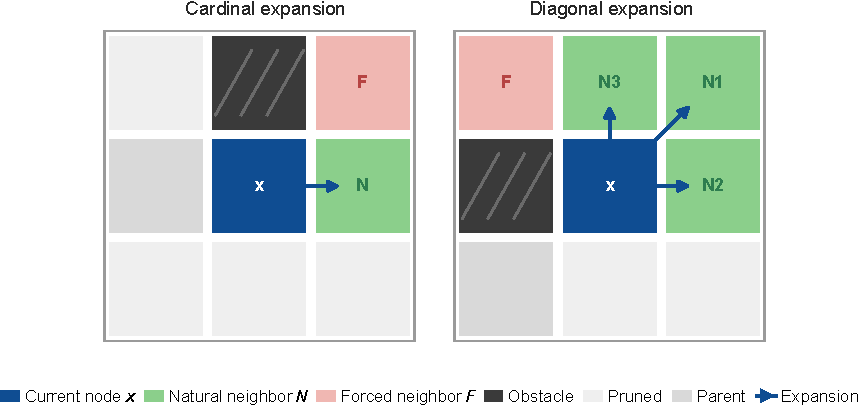
\includegraphics[width=3.0in]{figures/jps_pruning}
\caption{Illustration of the JPS neighbor-pruning rules.}
\label{fig:jps_pruning}
\end{figure}

Conventional A* expands neighbors cell by cell, so in large open regions the number of expanded nodes grows in proportion to the map area. To this end, this paper adopts an improved A* algorithm based on Jump Point Search (JPS)~\textcolor{blue}{\cite{ref11,ref12}}. JPS exploits grid symmetry to prune neighbors: along the expansion direction, only natural neighbors and forced neighbors induced by obstacles are retained; the jump function $\mathrm{jump}(r, c, dr, dc)$ advances along the given direction until the goal is reached, an obstacle is encountered, or a forced neighbor is discovered, and intermediate nodes are not inserted into the open set; jump-point costs are accumulated by Manhattan or diagonal distance; after the search completes, the path is recovered by backtracking parent pointers and filled in by straight-line interpolation between adjacent jump points. The pruning rules are illustrated in Fig.~\textcolor{blue}{\ref{fig:jps_pruning}}. On this basis, three improvements are made in this paper.

Owing to the jumping nature of JPS, diagonal moves in the reconstructed path may cut across obstacle corners. To this end, the proposed algorithm detects such cases during path reconstruction and replaces the corresponding moves with L-shaped paths along the grid boundary, thereby avoiding collisions.

\subsubsection{Tie-Breaking Strategy}

When multiple nodes in the open set share the same $f$-value, the selection order of standard A* depends on the specific implementation (typically first-in-first-out or random) and is essentially arbitrary. However, among nodes with identical $f$-values, a node with a smaller $h$-value has a larger actual cost $g = f - h$, i.e., it lies farther from the start and closer to the goal. Expanding such nodes first steers the search toward the goal without affecting the optimality guarantee. Accordingly, the improved A* algorithm proposed in this paper adopts the tie-breaking rule ``when $f$-values are equal, prefer the node with the smaller $h$-value.'' The node comparison rule is defined as
\begin{equation}
\begin{cases}
n_1, & f(n_1) < f(n_2) \\
n_2, & f(n_1) > f(n_2) \\
n_1, & f(n_1) = f(n_2) \land h(n_1) < h(n_2) \\
n_2, & f(n_1) = f(n_2) \land h(n_1) > h(n_2)
\end{cases}
\label{eq:tbreak}
\end{equation}

In physical terms, the evaluation function $f(n) = g(n) + h(n)$ implies that when two nodes share the same $f$-value, the one with the larger $g$ is farther from the start, whereas the one with the smaller $h$ is closer to the goal. Prioritizing such nodes biases the search toward the goal and reduces ineffective exploration in regions away from the goal.

\subsection{Path Post-Processing}
\label{subsec:post}

The path obtained by JPS search consists of a sequence of grid-center points; it contains redundant intermediate points and is composed of discrete horizontal and vertical segments, resulting in insufficient smoothness. This section proposes a two-stage processing approach to resolve these issues.

\subsubsection{Safety-Aware Path Simplification}

Conventional path simplification methods, such as corner pruning, directly connect non-adjacent nodes on the path and skip intermediate points to reduce the number of path points. However, such methods typically only check whether the connecting segment crosses obstacles and ignore the safety margin between path points and obstacles; in obstacle-dense regions this may cause paths to pass excessively close to obstacles. To this end, this section proposes a safety-distance-aware path simplification algorithm, whose core idea is to maintain a minimum safety distance between the path and obstacles during simplification.

The algorithm processes the input path in a four-step procedure. First, the nodes at which the direction changes are identified from the path: while keeping the start and end points, the connection directions of each intermediate node with its predecessor and successor are computed, and nodes whose forward and backward connection directions differ are marked as corner points $C_i$. Second, starting from the current corner $C_i$, the subsequent corners $C_j$ ($j > i$) are scanned forward; each segment $C_i \to C_j$ is verified against the safety-distance constraint via the safety check, the intermediate corners are skipped, and the farthest reachable corner $j^{*}$ is recorded as the new anchor. This greedy strategy maximizes the single-step simplification while preserving safety. On this basis, after the greedy step determines the farthest reachable corner $j^{*}$, it checks whether a skipped corner $k$ ($i < k < j^{*}$) can reach a farther corner $j'$ ($j' > j^{*}$) directly via a safe segment; if so, the route $(k, j')$ is recorded. Subsequently, the lengths of the two routes are compared: route A has length $d(C_i, C_{j^{*}}) + d(C_{j^{*}}, C_{j'})$, i.e., reaching $j^{*}$ first and then continuing to $j'$; route B has length $d(C_i, C_k) + d(C_k, C_{j'})$, i.e., bypassing $j^{*}$ and routing through $k$. If route B is shorter, the intermediate corner $C_k$ is retained; otherwise, only the greedy result $C_{j^{*}}$ is kept. This comparison ensures that intermediate-corner exploration does not come at the cost of path efficiency. Algorithm~\textcolor{blue}{\ref{alg:simplify}} gives the pseudocode of the path simplification algorithm.

\begin{algorithm}[!t]
\caption{Safety-distance-aware path simplification}
\label{alg:simplify}
\begin{spacing}{0.9}
\begin{algorithmic}[1]
\REQUIRE grid path $P = [P_1, \ldots, P_N]$, occupancy grid, safety margin $d_{\mathrm{safe}}$
\ENSURE simplified path $P_s$ ($|P_s| \leq N$)
\STATE $C \gets$ the corner points of $P$ where the direction changes, plus the two endpoints;
\STATE $P_s \gets [C_1]$; $\; i \gets 1$;
\WHILE{$i < |C|$}
\STATE $j^{*} \gets$ the farthest corner reachable from $C_i$ by a collision-free segment; \quad\textit{greedy forward scan}
\IF{$j^{*} = |C|$}
\STATE append $C_{|C|}$ to $P_s$ and break;
\ENDIF
\STATE $(k^{*}, j') \gets$ among all skipped corners $k$ ($i < k < j^{*}$) and farther corners $j$ ($j^{*} < j \leq |C|$), the pair with the largest $j$ such that the segment $C_k \to C_j$ is collision-free;
\IF{$k^{*}$ exists and $d(C_i, C_{k^{*}}) + d(C_{k^{*}}, C_{j'}) < d(C_i, C_{j^{*}}) + d(C_{j^{*}}, C_{j'})$}
\STATE append $C_{k^{*}}$ and $C_{j'}$ to $P_s$, and set $i \gets j'$; \quad\textit{route through the intermediate corner}
\ELSE
\STATE append $C_{j^{*}}$ to $P_s$, and set $i \gets j^{*}$;
\ENDIF
\ENDWHILE
\RETURN $P_s$;
\end{algorithmic}
\end{spacing}
\end{algorithm}

The safety-check function is implemented by dense cell-wise sampling: sample points are densely drawn along the segment from $p_1$ to $p_2$, and for each sample point its distance to the nearest obstacle-cell boundary is computed. If the distance of any sample point is smaller than the safety threshold $d_{\mathrm{safe}}$, the connection is deemed unsafe. The distance from a point to a cell boundary is given by
\begin{equation}
\begin{split}
d_x &= \max\left(0,\; |x_p - x_c| - 0.5\right)\\
d_y &= \max\left(0,\; |y_p - y_c| - 0.5\right)
\end{split}
\label{eq:dxymax}
\end{equation}

\begin{equation}
d(p, \mathrm{cell}) = \sqrt{d_x^2 + d_y^2}
\label{eq:dist}
\end{equation}
where $p = (x_p, y_p)$ is the sample point under the grid-to-continuous coordinate mapping described above, and $(x_c, y_c)$ is the center coordinate of the obstacle cell. The $\max(0, \cdot)$ operator handles the case in which the sample point has already fallen within the horizontal or vertical extent of the cell along a given axis. When the computed distance $d(p, \mathrm{cell})$ is smaller than the set safety-distance threshold $d_{\mathrm{safe}}$, the sample point has entered the safety exclusion zone of the obstacle cell.

\subsubsection{Arc-Length Parameterized Cubic Spline Smoothing}

Although the simplified path has removed redundant points, the output path is not sufficiently smooth and can hardly reflect the actual traveled distance of the motion. To this end, this paper adopts arc-length parameterized cubic spline smoothing, using the cumulative Euclidean distance between path points rather than the point index as the parameter, so that the parameter space remains consistent with the actual geometric space. The first step of the smoothing process is densification of sparse segments: for sparse segments whose adjacent points are separated by more than 2 grid units, $\lfloor \ell / 2 \rfloor$ intermediate points are linearly interpolated along the segment between the two endpoints. The purpose of densification is to provide the spline with sufficient control points and to prevent the Runge phenomenon on long straight segments caused by an insufficient number of control points, which would otherwise cause the curve to deviate from the intended polyline or even clip obstacle corners. The second step is arc-length parameterization. Let the densified path-point sequence be $\{P_0, P_1, \ldots, P_M\}$, where $P_i = (x_i, y_i)$ are continuous coordinates. The cumulative chord-length parameters are computed as $s_0 = 0$ and $s_i = s_{i-1} + \|P_i - P_{i-1}\|_2$ ($i = 1, 2, \ldots, M$). Cubic spline interpolation is then performed for $x(s)$ and $y(s)$ separately with $s$ as the independent variable, yielding the parametric curve $(x(s), y(s))$. On each subinterval $[s_i, s_{i+1}]$, the cubic spline is a cubic polynomial that guarantees continuity of the first- and second-order derivatives, and hence continuity of the curve curvature. The third step is equal arc-length resampling. The final smoothed path-point sequence is generated by uniformly sampling along the arc-length parameter $s$ at an interpolation density $\rho$. Because $s$ is approximately linearly related to the actual geometric distance, equal arc-length sampling ensures a uniform spatial distribution of path points and avoids the problem of conventional equal-parameter sampling, which places points densely at high curvature and sparsely at low curvature. Algorithm~\textcolor{blue}{\ref{alg:smooth}} gives the pseudocode of the smoothing algorithm.

\begin{algorithm}[!t]
\caption{Arc-length parameterized cubic spline smoothing}
\label{alg:smooth}
\begin{spacing}{0.9}
\begin{algorithmic}[1]
\REQUIRE grid path $P = [P_1, \ldots, P_N]$, density $\rho$ (default $10$)
\ENSURE smoothed continuous path $Q = [Q_1, \ldots, Q_M]$ in $[x, y]$
\STATE convert each grid point $P_i = (r_i, c_i)$ to continuous coordinates $(x_i, y_i) = (c_i - 0.5,\; r_i - 0.5)$;
\FOR{each consecutive pair whose segment length exceeds $2$}
\STATE insert $\lfloor \mathrm{length} / 2 \rfloor$ equally spaced intermediate points along the segment; \quad\textit{densification to prevent spline overshoot}
\ENDFOR
\STATE compute the cumulative chord length $t_1 = 0$, $t_i = t_{i-1} + \|P_i - P_{i-1}\|_2$; \quad\textit{arc-length parameter}
\STATE remove duplicate $t$ values to keep strict monotonicity;
\STATE fit cubic splines $x(t)$ and $y(t)$ through the densified points;
\STATE sample $x(t)$ and $y(t)$ at $\rho$ points per segment to obtain $Q$;
\RETURN $Q$;
\end{algorithmic}
\end{spacing}
\end{algorithm}

\subsubsection{Pipeline Integration}

The above post-processing operations are integrated as a pipeline: the JPS search outputs the raw grid path $\to$ SimplifyPath removes redundant points $\to$ SmoothPath generates a smooth continuous-coordinate path. The entire pipeline is completed in one pass, and the resulting path possesses both a safety margin and smoothness. The rationale of this two-stage design is that path simplification and spline smoothing address two distinct dimensions of path quality. Safety-aware path simplification reduces the number of path points and lowers the complexity of subsequent computation while guaranteeing the safety margin of the path; smoothing converts the discrete grid path into a continuous curve, enabling the robot to track the path with a smooth motion trajectory. If smoothing is applied without prior simplification, the spline must handle a large number of redundant control points, which not only increases computational cost but may also produce unstable curve shapes due to excessively dense control points. A comparison of the path before and after post-processing is shown in Fig.~\textcolor{blue}{\ref{fig:pipeline}}.

\begin{figure}[!t]
\centering
\subfloat[Original path and simplified path]{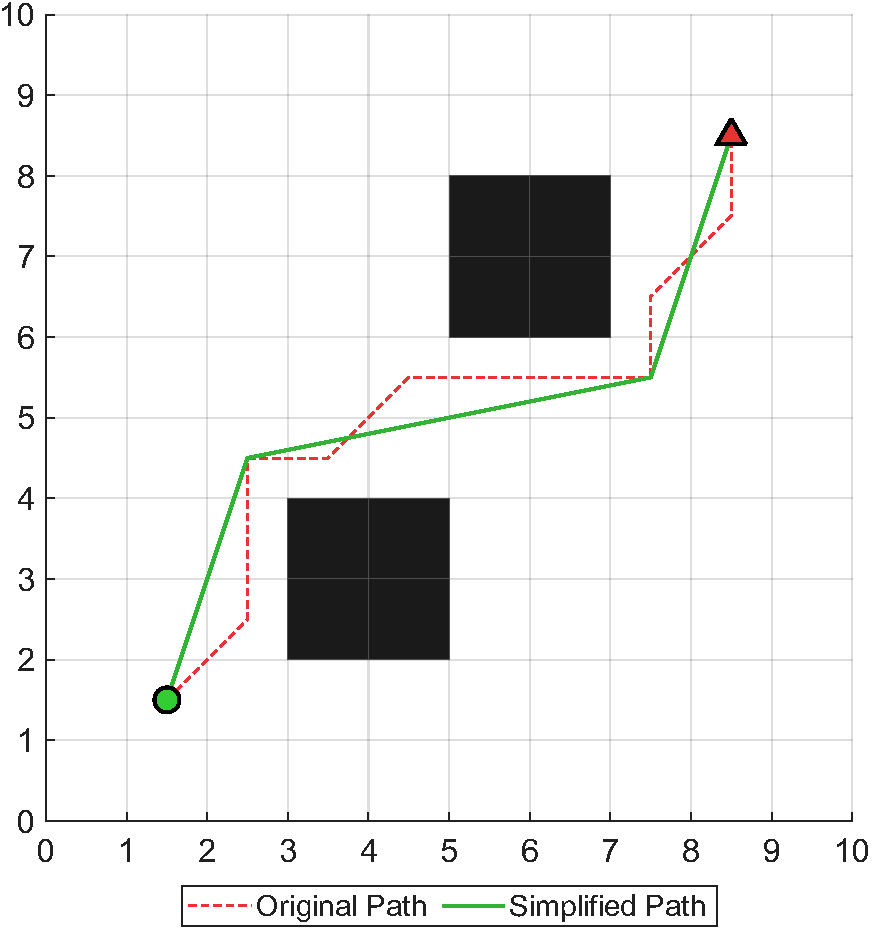
\includegraphics[width=1.55in]{figures/SimplifyPath}%
\label{fig:pipeline_a}}%
\hfil
\subfloat[Simplified path and smoothed path]{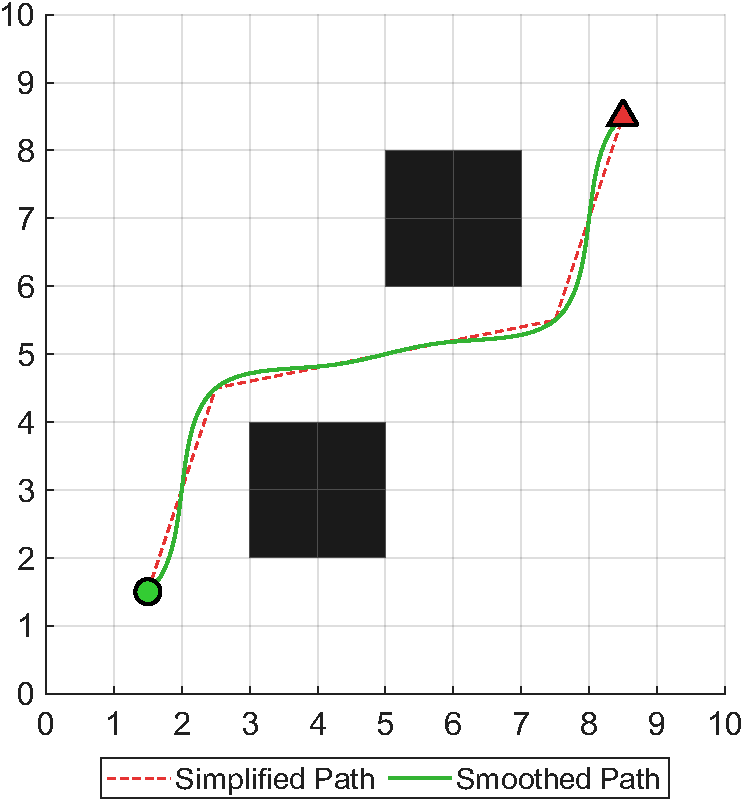
\includegraphics[width=1.55in]{figures/SmoothPath}%
\label{fig:pipeline_b}}
\caption{Comparison of the path at the individual stages of the pipeline.}
\label{fig:pipeline}
\end{figure}

\subsection{Improved Open Traveling Salesman Ant Colony Optimization}
\label{subsec:aco}

The ordering layer of the framework solves the open traveling salesman problem on the cost matrix produced by the global planning layer. Given $N$ points consisting of a fixed start point $S$, $K$ intermediate goal points $\{T_1, \dots, T_K\}$, and a fixed end point $G$, the objective is to find the permutation of the $K$ goal points that minimizes the total path cost. On the basis of the ant colony optimization (ACO) metaheuristic, this paper introduces six integrated mechanisms, which are described in turn in this subsection.

\subsubsection{Virtual-Node Encoding of the Open Traveling Salesman Problem}
\label{subsec:virtual}

For the open traveling salesman problem, the start point $S$ and the end point $G$ are distinct physical locations specified by the task, and optimization is performed only on the ordering of the $K$ intermediate goal points. A naive full-permutation encoding produces invalid solutions with misaligned endpoints; if the start and end are pinned in the encoding, $S$ and $G$ are excluded from the pheromone model and local search, limiting the ability to optimize the complete solution. To this end, this paper adopts the virtual-node method to convert the open traveling salesman problem into a standard closed traveling salesman problem~\textcolor{blue}{\cite{ref32}}.

A virtual node $V = N + 1$ is introduced, and an extended cost matrix $\mathbf{D}_{\mathrm{ext}}$ of size $(N+1) \times (N+1)$ is constructed:
\begin{equation}
\mathbf{D}_{\mathrm{ext}}(i, j) =
\begin{cases}
0, & \{i, j\} = \{V, 1\} \\
0, & \{i, j\} = \{V, N\} \\
\mathrm{BIG}, & \begin{aligned}[t]
& (i = V \lor j = V) \land \\
& \{i, j\} \cap \{1, N\} = \varnothing
\end{aligned} \\
\mathbf{D}(i, j), & \text{otherwise}
\end{cases}
\label{eq:dext}
\end{equation}
where $\mathrm{BIG} = 2(N+1) \cdot \max_{i,j} \mathbf{D}(i,j)$ is a penalty strictly larger than the cost of any feasible tour, ensuring that the virtual node is not directly connected to any intermediate goal point in any near-optimal tour and is therefore forced to be adjacent only to the start and the end.

The solver runs on $\mathbf{D}_{\mathrm{ext}}$ as a standard closed traveling salesman problem, and the pheromone matrix $\bm{\tau}$ covers the full $(N+1)\times(N+1)$ space. After the solver converges, $V$ is removed from the best tour, the remaining nodes are read in tour order and reordered so that the start comes first and the end last, yielding the open visiting sequence. Relative to the boundary-fixed encoding, this transformation lets the start and end fully participate in pheromone updates and local search, allows closed-tour operators to be applied uniformly, and makes the cost evaluation simply the tour sum on $\mathbf{D}_{\mathrm{ext}}$. The heuristic visibility matrix $\bm{\eta}$ is defined as
\begin{equation}
\eta_{ij} =
\begin{cases}
\mathrm{BIG}, & \{i, j\} = \{V, 1\} \text{ or } \{V, N\} \\
\dfrac{1}{\mathbf{D}_{\mathrm{ext}}(i,j)}, & \mathbf{D}_{\mathrm{ext}}(i,j) > 0 \\
0, & \text{otherwise}
\end{cases}
\label{eq:eta}
\end{equation}
i.e., the zero-cost edges incident to $V$ are assigned a large heuristic value that strongly attracts $V$ to its required neighbors, while other pairs take the reciprocal of the extended cost. The cost of a closed tour $\bm{\sigma} = (\sigma_1, \dots, \sigma_{N+1})$ is the sum of its edge costs, including the closing edge $\sigma_{N+1} \to \sigma_1$.

\subsubsection{Max--Min Ant System Pheromone Update with Dynamic Bounds}

The Max--Min Ant System (MMAS)~\textcolor{blue}{\cite{ref23}} restricts pheromone values to an explicit interval $[\tau_{\min}, \tau_{\max}]$ to prevent unilateral domination and extinction, and concentrates deposition on elite solutions. This paper adopts this mechanism and specifies a bound-initialization and update procedure matched to the cost scale.

In each iteration, all pheromone values are first evaporated as $\tau_{ij} \leftarrow (1 - \rho) \cdot \tau_{ij}$ ($\rho$ is the evaporation rate), and pheromone is then deposited on the iteration-best tour $\bm{\sigma}_{\mathrm{iter-best}}$ and the global-best tour $\bm{\sigma}_{\mathrm{global-best}}$, respectively, as
\begin{equation}
\tau_{ij} \leftarrow \tau_{ij} + \frac{Q}{C_{\mathrm{iter}}}, \qquad
\tau_{ij} \leftarrow \tau_{ij} + \frac{Q}{C_{\mathrm{global}}}
\label{eq:deposit}
\end{equation}
where $Q$ is the deposit constant and $C$ is the corresponding tour cost. The deposit amount is inversely proportional to the tour cost and is applied symmetrically to $(i,j)$ and $(j,i)$. After deposition, the pheromone is clamped to the current interval, whose bounds are given dynamically by the global-best cost:
\begin{equation}
\tau_{\max} = \frac{1}{\rho \cdot C_{\mathrm{global}}}, \qquad
\tau_{\min} = \frac{\tau_{\max}}{N+1}
\label{eq:taumax}
\end{equation}
The initial pheromone is set to a uniform value $\tau_0$, corresponding to bounds $\tau_{\max}^{0} = 1/(\rho \cdot \tau_0 \cdot (N+1))$ and $\tau_{\min}^{0} = \tau_{\max}^{0}/(5(N+1))$, so that $\tau_0$ is not clipped during the early stage; a hard lower limit is additionally imposed on $\tau_{\min}$ to prevent low-frequency edges from underflowing to extinction under small-scale costs. Within a single iteration the update order is: evaporate, deposit according to Eq.~\textcolor{blue}{\eqref{eq:deposit}}, clamp, and recompute the bounds according to Eq.~\textcolor{blue}{\eqref{eq:taumax}}.

Dynamic bound updates are critical: as the search discovers better tours, the decrease in $C_{\mathrm{global}}$ increases $\tau_{\max}$, allowing the algorithm to express stronger confidence in its current best tour; the ratio $\tau_{\min}/\tau_{\max} = 1/(N+1)$ maintains a constant relative gap, preserving a baseline exploration probability for every edge.

\subsubsection{Ant Colony System Style Pseudo-Random Transition Rule}

The pseudo-random proportional rule of the Ant Colony System (ACS)~\textcolor{blue}{\cite{ref22}} greedily selects the best candidate with a controllable probability and explores by roulette selection otherwise, balancing convergence and diversity. This paper adopts this rule as the transition mechanism during the path-construction phase.

Concretely, when an ant at the current node $u$ selects the next node from the unvisited candidate set $\mathcal{U}$, it first computes the score of each candidate as $\mathrm{score}(v) = (\tau_{uv})^{\alpha} \cdot (\eta_{uv})^{\beta}$, where $\alpha$ and $\beta$ are the pheromone and heuristic weight exponents, respectively. It then exploits with probability $q_0$, deterministically selecting the highest-scoring candidate $v_{\mathrm{next}} = \arg\max_{v \in \mathcal{U}} \mathrm{score}(v)$, and explores with probability $1 - q_0$ by roulette selection, in which each candidate $v$ is chosen with probability $\mathrm{score}(v) / \sum_{u \in \mathcal{U}} \mathrm{score}(u)$. If all scores are zero, i.e., all remaining nodes are unreachable, an unvisited candidate is selected at random as a fallback.

As can be seen, a larger $q_0$ causes more construction steps to adopt greedy selection and thus accelerates convergence, whereas a smaller $q_0$ increases the proportion of random exploration. Pairwise distances in the obstacle-constrained cost matrix usually exhibit spatial locality, so the heuristic $\bm{\eta}$ provides reasonably reliable guidance; a moderate-to-high greedy probability therefore remains beneficial for convergence while preserving diversity.

\subsubsection{Variable Neighborhood Descent Local Search Accelerated by a Candidate List}
\label{subsec:vnd}

Although the paths constructed by ants are guided by pheromone and heuristic information, they are not necessarily locally optimal. A natural improvement is to apply local search to the tours constructed by a subset of the ants in each generation, further refining solution quality by systematically examining neighboring permutations. Variable Neighborhood Descent (VND)~\textcolor{blue}{\cite{ref24}} is precisely such a class of methods: it invokes multiple neighborhood structures in sequence, each corresponding to a class of path transformations, and switches to the next structure when the current one can no longer improve the solution, until no neighborhood yields a better solution. Existing studies have shown that hybridizing MMAS or ACS with VND is highly effective for vehicle routing problems~\textcolor{blue}{\cite{ref25}}. However, standard VND must examine $O(K^2)$ neighborhoods for each operator, and the computational cost rises rapidly as the number of goal points grows, becoming a major bottleneck. Further observation reveals that many of these examinations are fruitless: when a pair of distant nodes participates in a 2-opt exchange, it rarely yields an improvement in tour cost.

To this end, this paper first introduces a precomputed candidate list to filter out unpromising neighborhood evaluations, an idea widely used in local search for the traveling salesman problem~\textcolor{blue}{\cite{ref26}}. Specifically, for each node its $k$ nearest neighbors are preselected according to the extended cost matrix $\mathbf{D}_{\mathrm{ext}}$ and stored in a Boolean matrix. During local search, the cost change of a move is computed only when the new edges it introduces are related to candidate neighbors; otherwise the evaluation is skipped.

On this basis, VND is performed on the closed tour of the $N+1$ nodes including the virtual node, alternating among three neighborhood operators in a fixed order:
\begin{enumerate}
\item \textbf{2-opt}: reverses a contiguous subsequence of the path, replacing the original edges $(u, u^{+})$ and $(v, v^{+})$ with $(u, v)$ and $(u^{+}, v^{+})$, thereby eliminating path crossings typical of Euclidean-like costs.
\item \textbf{Relocate}: takes a node from its current position and inserts it elsewhere in the tour, shifting the intermediate nodes accordingly, which corrects cases where a node has been placed in the wrong path segment.
\item \textbf{Swap}: exchanges two nodes while keeping all others unchanged, which is applicable when two nodes happen to be assigned to each other's better positions.
\end{enumerate}
The above operators all follow the first-improvement principle in the VND loop. In each round the 2-opt, relocate, and swap operators are each executed once in the fixed order; whenever any operator yields an improvement, a new round starts, and the local search terminates when none of the three operators improves the solution in a round. Because the problem is defined on a closed tour, when a swap involves the first and last adjacent nodes of the tour, the wrap-around connection is handled through cyclic predecessor and successor indices, and adjacent swaps that cross the closing edge evaluate the three involved edges separately, rather than reusing the adjacency test for a linear path.

In terms of complexity, without pruning each VND operator would examine $O((N+1)^2)$ candidate moves; with the candidate list, each node participates in only about $O(k)$ neighborhood checks, reducing the complexity of a single operator to $O((N+1)\cdot k)$. When $k$ is much smaller than $N+1$, this effectively reduces the computation relative to full-neighborhood enumeration.

Algorithm~\textcolor{blue}{\ref{alg:vnd}} gives the complete pseudocode of candidate-list-accelerated VND, and the full flow of the VND neighborhood search is shown in Fig.~\textcolor{blue}{\ref{fig:vnd_flow}}.

\begin{algorithm}[!t]
\caption{Candidate-list-accelerated variable neighborhood descent}
\label{alg:vnd}
\begin{spacing}{0.9}
\begin{algorithmic}[1]
\REQUIRE closed tour $\bm{\sigma} = [\sigma_1, \dots, \sigma_{N+1}]$, extended cost matrix $\mathbf{D}_{\mathrm{ext}}$, candidate boolean matrix $\mathbf{C}$
\ENSURE improved tour $\bm{\sigma}$ and its cost
\STATE $\mathrm{cost} \gets$ the cost of tour $\bm{\sigma}$ under $\mathbf{D}_{\mathrm{ext}}$;
\REPEAT
\STATE $\mathrm{improved} \gets$ false;
\STATE $[\bm{\sigma}, \mathrm{cost}, \mathrm{ok}] \gets$ apply the 2-opt operator with candidate-list pruning (first-improvement);
\STATE $\mathrm{improved} \gets \mathrm{improved}$ or ok;
\STATE $[\bm{\sigma}, \mathrm{cost}, \mathrm{ok}] \gets$ apply the relocate operator with candidate-list pruning;
\STATE $\mathrm{improved} \gets \mathrm{improved}$ or ok;
\STATE $[\bm{\sigma}, \mathrm{cost}, \mathrm{ok}] \gets$ apply the swap operator with candidate-list pruning;
\STATE $\mathrm{improved} \gets \mathrm{improved}$ or ok;
\UNTIL{$\mathrm{improved} = \mathrm{false}$}
\STATE $\mathrm{cost} \gets$ the exact cost of the final tour $\bm{\sigma}$;
\RETURN $\bm{\sigma}$, $\mathrm{cost}$;
\end{algorithmic}
\end{spacing}
\end{algorithm}

\begin{figure}[!t]
\centering
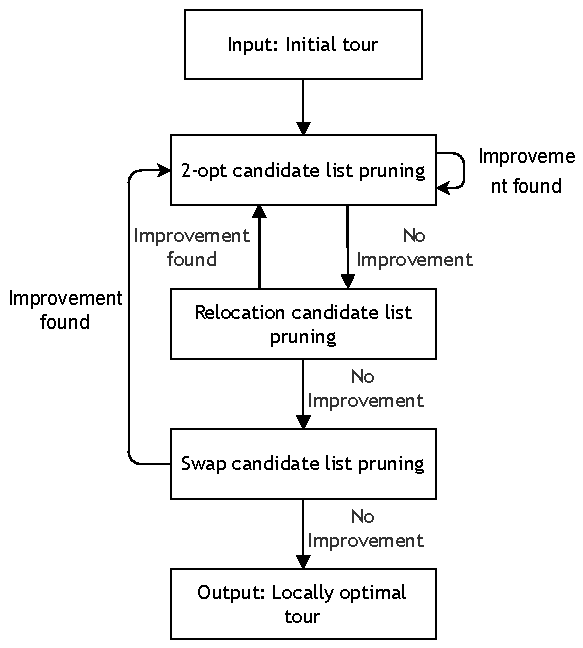
\includegraphics[width=3in]{figures/fig03_vnd_flow.pdf}
\caption{VND neighborhood search sequence flowchart.}
\label{fig:vnd_flow}
\end{figure}

\subsubsection{Sigmoid Progressive Local Search Schedule}
\label{subsec:sigmoid}

Even with candidate-list acceleration, VND local search still requires a relatively long computation time. If local search were applied to all ants in every generation, the resources of early iterations would often be wasted, since the population has not yet identified promising regions of the search space and refining low-quality tours yields limited benefit; later on, when pheromone has concentrated on high-quality regions, intensive local search becomes critical for polishing the solution. Applying local search to a fixed proportion of ants throughout the run is therefore not ideal---a low proportion slows convergence, whereas a high proportion spends computation on immature solutions. Accordingly, this paper dynamically adjusts the proportion of ants that accept VND local search along a sigmoid function:
\begin{equation}
\mathrm{optRatio}(t) = y_{\min} + (y_{\max} - y_{\min}) \cdot \frac{t^{a}}{t^{a} + (1 - t)^{a}}
\label{eq:sigmoid}
\end{equation}
where $t = (\mathrm{iter} - x_L) / (x_R - x_L)$ is the normalized position of the current iteration within the transition interval $[x_L, x_R]$; $y_{\min}$ and $y_{\max}$ are the lower and upper bounds of the local-search proportion in the early and late stages, and $a$ controls the steepness of the sigmoid curve. When $t$ precedes $x_L$, $\mathrm{optRatio}$ takes $y_{\min}$; after $x_R$ it is held at $y_{\max}$; inside the interval the proportion changes smoothly along the sigmoid curve.

This schedule smoothly shifts the search from broad exploration in the early stage to intensive refinement of high-quality solutions in the late stage, while a subset of the ants maintains construction diversity. The S-curve of $\mathrm{optRatio}(t)$ is shown in Fig.~\textcolor{blue}{\ref{fig:sigmoid}}.

After the number of ants $n_{\mathrm{opt}} = \lceil n_{\mathrm{ants}} \cdot \mathrm{optRatio} \rceil$ that accept local search in the current round is determined, the specific individuals must still be selected. This paper adopts an elite--random hybrid: $n_{\mathrm{elite}} = \lceil n_{\mathrm{opt}} \cdot r_{\mathrm{elite}} \rceil$ top-ranked elite individuals are optimized first to reinforce the polishing of high-quality solutions, and the remaining $n_{\mathrm{random}} = n_{\mathrm{opt}} - n_{\mathrm{elite}}$ individuals are drawn at random from the non-elite population and optimized as well, so that promising regions outside the elite may still be discovered and a balance between exploitation and exploration is maintained. Here $r_{\mathrm{elite}}$ is the elite proportion parameter.

\begin{figure}[!t]
\centering
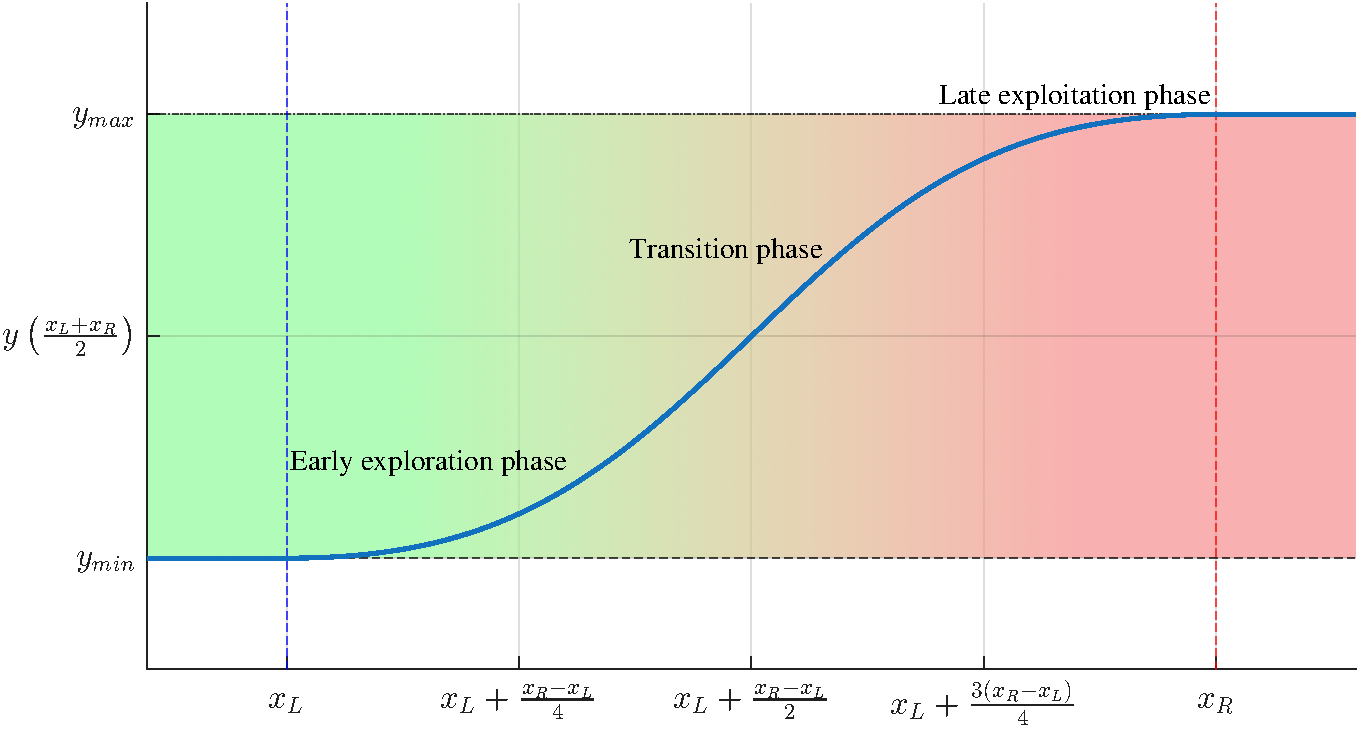
\includegraphics[width=2.5in]{figures/S_optRatio}
\caption{Sigmoid curve of $\mathrm{optRatio}(t)$ versus the iteration count.}
\label{fig:sigmoid}
\end{figure}

\subsubsection{Adaptive Stopping Criterion}

The algorithm uses the maximum iteration count $n_{\mathrm{iter}}$ as the budget ceiling so that difficult instances can still converge. On easy instances, however, convergence usually occurs far earlier, and further iterations only add computation; stopping too early, conversely, may miss better solutions. The stopping criterion must therefore distinguish ``fully converged'' from ``temporarily not improving'', and two complementary indicators are monitored simultaneously.

The first indicator is population homogeneity. When the ant colony has converged to a narrow region, the tour costs of different ants become close to each other, which can be characterized by the coefficient of variation $\mathrm{CV} = \sigma_{\mathrm{costs}} / \mu_{\mathrm{costs}}$. When $\mathrm{CV}$ falls below the preset threshold $\varepsilon_{\mathrm{CV}}$, the population is regarded as homogeneous and the chance of discovering new solutions is low.

The second indicator is stagnation of the best solution. Even if the population still has some diversity, the global best may remain near a local optimum for a long time. The algorithm therefore records the number of consecutive iterations without improvement of the global-best cost and terminates once the preset limit $\mathrm{stagn}_{\max}$ is reached.

To reduce the risk of premature stopping, the two criteria are enabled only after $\mathrm{minIter}$ iterations have been completed, because early in the search the cost variance is large and the global best is still improving rapidly, so monitoring convergence too early can misclassify normal fluctuations as convergence.

\subsubsection{Integration Summary}

\begin{figure}[!t]
\centering
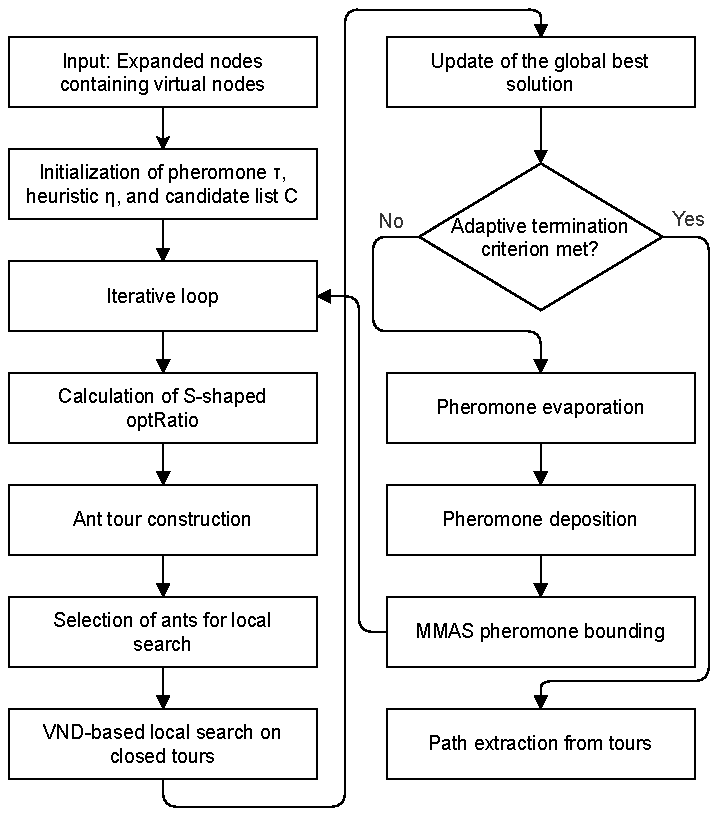
\includegraphics[width=\columnwidth]{figures/fig05_aco_flow.pdf}
\caption{Overall flowchart of the improved ant colony optimization.}
\label{fig:aco_flow}
\end{figure}

In summary, the MMAS-VND-CL algorithm organizes each mechanism into a single iterative search pipeline: the extended cost matrix $\mathbf{D}_{\mathrm{ext}}$ is defined on the $N+1$ nodes including the virtual node, and both the pheromone model and the local search operate in this space. The main steps of a single iteration are as follows:
\begin{enumerate}
\item The S-curve determines the proportion of ants that accept local search in the current round;
\item All ants each construct a Hamiltonian tour covering the $N+1$ nodes according to the ACS-style pseudo-random transition rule;
\item A subset of ants is selected by the elite--random hybrid strategy, and candidate-list-accelerated VND local search is applied to their tours;
\item The current global-best tour is updated, and the adaptive stopping criterion is checked;
\item If the search continues, the pheromone is first evaporated, then deposited on the iteration-best and global-best tours, and finally clamped dynamically according to the MMAS rule.
\end{enumerate}
The search ends when the adaptive stopping condition is met. Upon termination, the virtual node $V$ is removed from the best tour, and the remaining nodes are reordered so that the start comes first and the end last, yielding the final open-path visiting sequence. The overall flow of the MMAS-VND-CL algorithm is shown in Fig.~\textcolor{blue}{\ref{fig:aco_flow}}.

\subsection{Cooperative Optimization Framework}
\label{subsec:coop}

The preceding subsections have presented the improved A* path-finding layer and the MMAS-VND-CL ordering layer. This subsection connects the two into a complete pipeline: first construct the obstacle-constrained cost matrix, then optimize the visiting order on that matrix, and finally retrieve and concatenate the segment paths in sequence into a complete trajectory.

The geometric layer constructs the cost matrix. Given the start point, the end point, and $K$ intermediate goal points (a total of $N$ points), the shortest collision-free path is computed for every point pair; after safety simplification and arc-length-parameterized cubic spline smoothing, the Euclidean arc lengths of the continuous trajectories form the cost matrix $\mathbf{D} \in \mathbb{R}^{N \times N}$. $\mathbf{D}$ is not a Euclidean distance matrix: its elements correspond to the true obstacle-constrained traversal lengths. Pricing by smoothed arc length rather than accumulated grid steps weakens the discretization staircase effect and makes the ordering criterion closer to the actually executed travel. Construction requires $O(N^2)$ planner calls; in engineering practice a point-pair path cache can avoid repeated searches. If a point pair has no feasible path, the corresponding element is set to $\mathbf{D}(i, j) = \infty$, and if any goal is unreachable from the start, the procedure aborts and reports failure.

The ordering layer optimizes the visiting order. This layer solves the open traveling salesman problem on the numeric matrix $\mathbf{D}$ alone, without access to the map or obstacle geometry, and returns the optimal visiting sequence $\bm{\pi}^{*} = (1, \pi_2, \dots, \pi_{K+1}, N)$ together with the total cost $C(\bm{\pi}^{*})$; the segment paths of adjacent point pairs are then retrieved from the cache in this order and concatenated into a complete collision-free continuous trajectory. When $K = 0$, the problem reduces to a single-pair shortest-path query, with order $[1, N]$ and cost $\mathbf{D}(1, N)$.

Separating the two layers allows the planner and the ordering solver to be replaced independently and compared layer by layer, while the cost matrix $\mathbf{D}$ compresses the obstacle-distance topology into a compact interface, so that the ordering layer retains obstacle-avoidance feasibility without touching the grid map. The information loss is that the solver cannot tell whether two segments share the same narrow corridor, but for the objective of minimizing total cost this representation is sufficient. End to end, the system completes cost-matrix construction, open traveling salesman solving, and path retrieval in sequence; the overall architecture is shown in Fig.~\textcolor{blue}{\ref{fig:system}}.

\begin{figure}[!htbp]
\centering
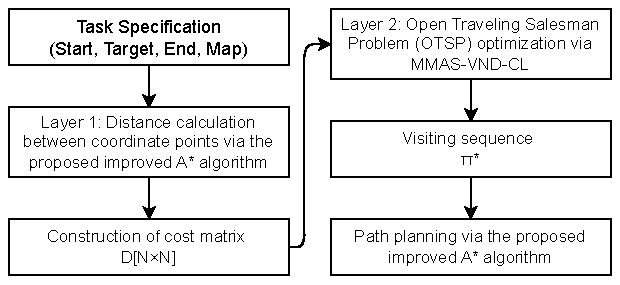
\includegraphics[width=\columnwidth]{figures/fig06_system.pdf}
\caption{Overall system architecture.}
\label{fig:system}
\end{figure}

\section{Experiments and Analysis}
\label{sec:exp}

After presenting the method design, this section validates the effectiveness of the proposed framework through simulation. The experiments are organized along several interconnected levels. First, the JPS-based improved A* planner is compared with common baselines in terms of global path-finding efficiency and path quality. Second, the sensitivity of MMAS-VND-CL to key hyperparameters is examined. Third, ablation experiments isolate the contribution of each constituent mechanism. Finally, different traveling-salesman solvers are combined with the improved A* planner to compare complete multi-goal traversal performance. All comparisons are repeated independently multiple times under a unified parameter policy, so that solution quality and statistical stability are both accounted for.

\begin{figure*}[!htbp]
\centering
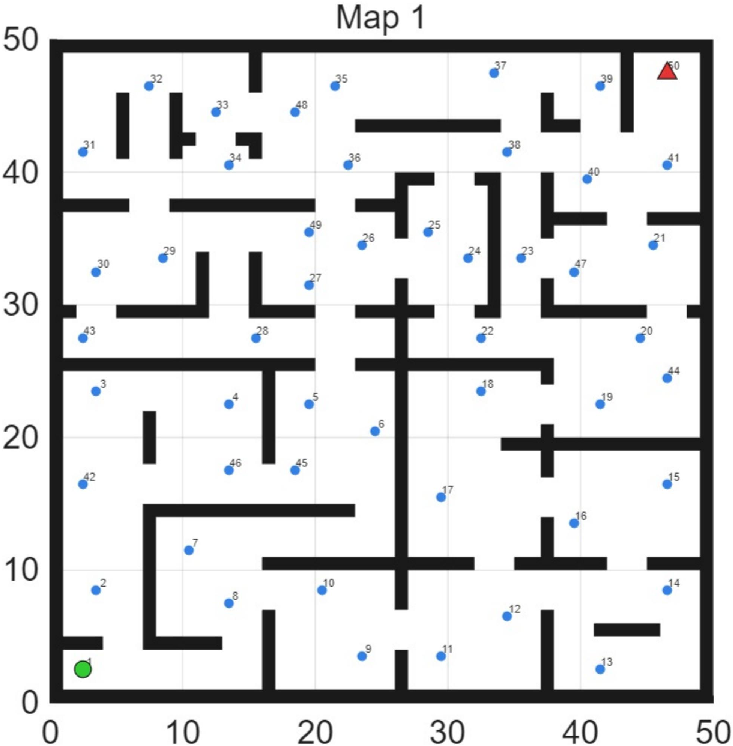
\includegraphics[height=3.7cm]{figures/Map_1}\hfil
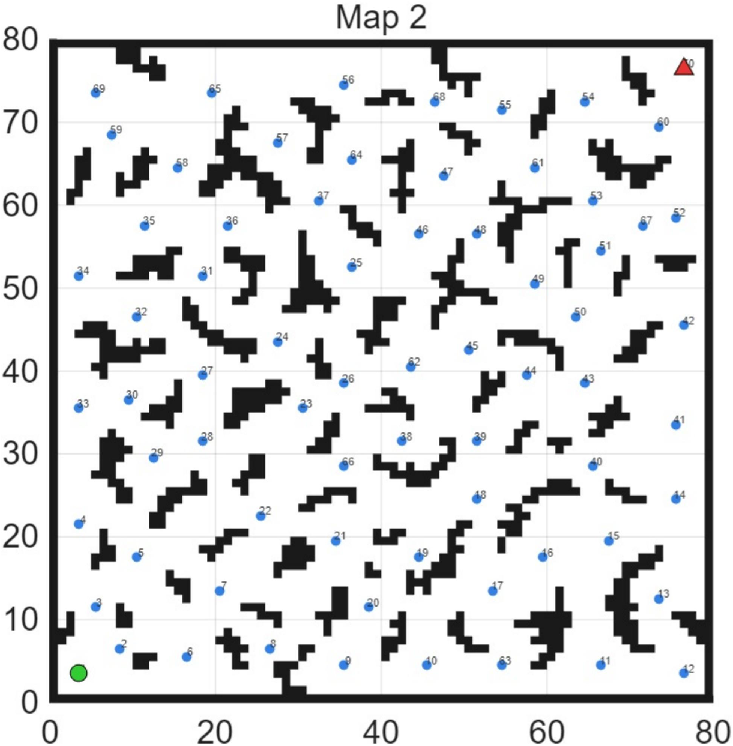
\includegraphics[height=3.7cm]{figures/Map_2}\hfil
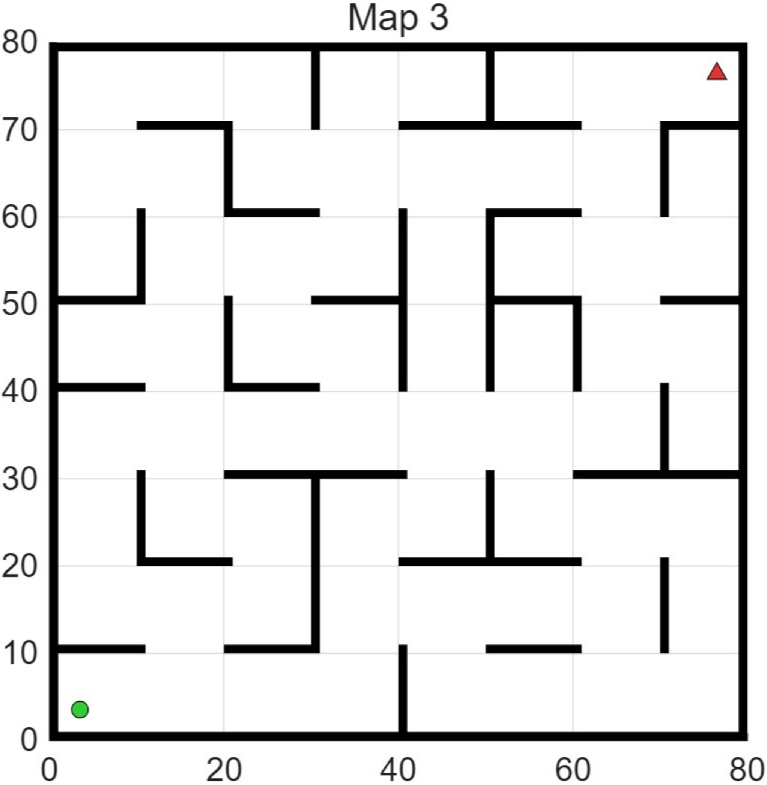
\includegraphics[height=3.7cm]{figures/Map_3}\hfil
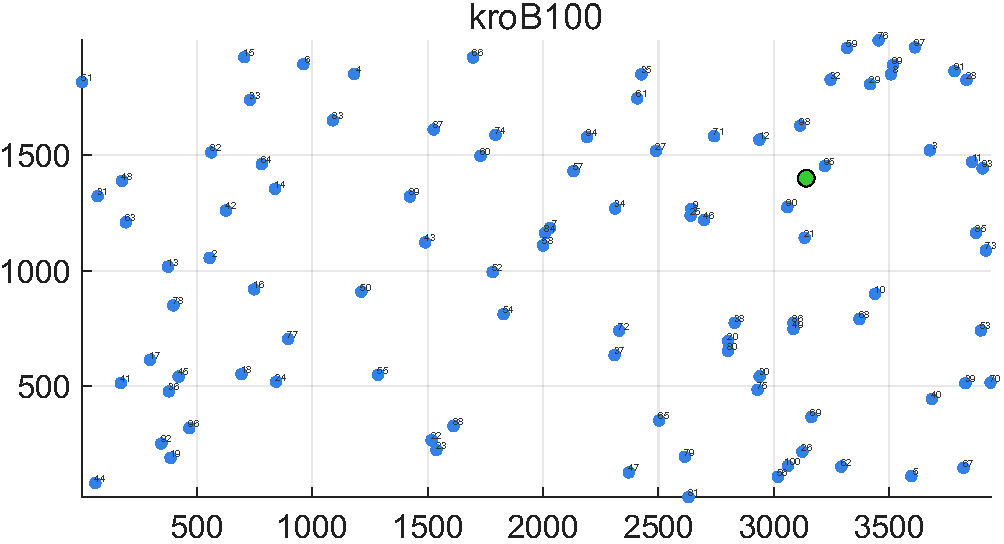
\includegraphics[height=3.7cm]{figures/Map_kroB100}
\caption{Schematic of the experimental environments. In Map~1 and Map~2, green circles denote the start point, red triangles the goal point, and blue numbered points the intermediate targets for multi-goal traversal; Map~3 provides only the start and goal; kroB100 shows the planar distribution of 100 cities, with green circles marking the endpoints of the open path.}
\label{fig:env_maps}
\end{figure*}

\subsection{Experimental Setup}

All experiments were conducted on a computer equipped with an Intel Core Ultra 5 125H processor and 32~GB of memory, using MATLAB R2025b as the software environment.

To cover different obstacle morphologies and problem scales, two classes of experimental scenarios were constructed, as illustrated in Fig.~\textcolor{blue}{\ref{fig:env_maps}}. One class consists of obstacle-laden grid maps (Map~1, Map~2, and Map~3), used to examine obstacle-avoiding path finding and multi-goal traversal. The other class is the standard TSPLIB instance kroB100, used solely to examine large-scale combinatorial ordering capability. In the figure, green circles denote the start point, red triangles the goal point, and blue numbered points the intermediate targets in the multi-goal traversal experiments. Map~1 and Map~2 simultaneously provide the intermediate targets required for multi-goal traversal; in the global path-planning comparison of Section~\textcolor{blue}{\ref{subsec:exp_plan}}, only the start and goal of each map are used for point-to-point planning, and no visit-order optimization over intermediate targets is involved.

The specific environment characteristics are as follows.

\begin{enumerate}

\item Map~1: a $50\times 50$ grid environment. Obstacles are dominated by relatively long horizontal and vertical wall segments, forming several corridor-connected ``room''-like cavities. The layout is broadly reminiscent of an urban block or an indoor partitioned floor plan, which is suitable for examining detour behavior and search efficiency under moderate obstacle density.

\item Map~2: an $80\times 80$ grid environment. Obstacles appear as irregular, high-density fragmented patches, and the free space is cut into numerous narrow, winding passages whose local traversability depends heavily on short-range obstacle avoidance, making the map useful for assessing robustness in cluttered environments.

\item Map~3: an $80\times 80$ maze environment. The wall segments are longer and roughly orthogonal, forming typical maze-like corridors with narrow passages and frequent turns. It is used only for the global path-planning comparison, so as to highlight the performance differences among pathfinding algorithms in a structured maze.

\item kroB100: the standard 100-city TSPLIB instance. Cities are given by planar coordinates, and the focus is on the visit-order optimization of a large set of targets. In this paper, both the start and the goal are set to city~1, so that the open path degenerates into a tour and can be compared directly with the published TSPLIB optimal tour length of 22141, serving as a calibration benchmark for combinatorial search capability at a scale of about one hundred points.

\end{enumerate}

The scales of the multi-goal traversal instances are as follows. Map~1 uses 50 navigation points including the start and the goal, and Map~2 uses 70 navigation points including the start and the goal. The start and the goal are respectively the first and last points of each instance's navigation-point sequence, and the grid coordinates of the navigation points are given by the numbered annotations in Fig.~\textcolor{blue}{\ref{fig:env_maps}}. The kroB100 instance contains all 100 cities.

\begin{table}[!ht]
\caption{Default Parameter Settings of the Proposed Algorithm}
\label{tab:params}
\centering
\scriptsize
\begin{tabular}{lccc}
\toprule
Module & Parameter & Symbol & Value \\
\midrule
\multirow{6}{*}{Original params}
& Number of ants & $n_{\mathrm{ants}}$ & 40 \\
& Pheromone weight & $\alpha$ & 1 \\
& Heuristic weight & $\beta$ & 2.0 \\
& Evaporation rate & $\rho$ & 0.25 \\
& Deposit constant & $Q$ & 225 \\
& Initial pheromone & $\tau_0$ & 0.1 \\
\midrule
\multirow{1}{*}{ACS}
& Greedy probability & $q_0$ & 0.45 \\
\midrule
\multirow{6}{*}{VND}
& Local search ratio & $y_{\max}$ & 0.4 \\
& \makecell{Local search transition\\interval} & $[x_L, x_R]$ & $[0, 30]$ \\
& Elite ratio & $r_{\mathrm{elite}}$ & 0.7 \\
& Candidate list size & $k$ & 9 \\
& Local search ratio lower bound & $y_{\min}$ & 0.0 \\
& S-curve steepness & $a$ & 2.0 \\
\midrule
\multirow{4}{*}{Adaptive stopping}
& Homogeneity threshold & $\varepsilon_{\mathrm{CV}}$ & $10^{-3}$ \\
& Stagnation limit & $\mathrm{stagn}_{\max}$ & 70 \\
& Minimum iterations & $\mathrm{minIter}$ & 30 \\
& Maximum iterations & $n_{\mathrm{iter}}$ & 800 \\
\bottomrule
\end{tabular}
\end{table}

Regarding the number of repetitions and the statistical protocol: in the global path-planning comparison, each algorithm is run 10 times on each map and the average computation time is reported. In the traveling-salesman-related experiments, each configuration is run 40 times, and the best cost, the mean convergence cost with standard deviation, the computation time, and the success rate are reported. The computation time of the traveling-salesman-related experiments is the solver time on a precomputed cost matrix and does not include the $O(N^2)$ cost-matrix construction or path post-processing.

For the parameter settings, the main parameters of the proposed MMAS-VND-CL algorithm take the default values listed in Table~\textcolor{blue}{\ref{tab:params}} throughout the paper.

The evaluation metrics include path length, computation time, number of expanded nodes (global planning only), best cost, mean convergence cost, success rate, and standard deviation. The sources of the reference best costs fall into two categories. The reference value of 22141 for kroB100 is the optimal tour length published by TSPLIB and is therefore an externally certified value. The reference values for Map~1 and Map~2 are 352.56 and 623.78, respectively, and correspond to the best observed values over all algorithms and all runs in this experiment. The success rate is defined as the fraction of runs that attain the reference best cost. Because the reference values for Map~1 and Map~2 come from observation rather than certified optima, a baseline success rate of 0\% should be understood as not attaining the best known value of this experiment, rather than as the absence of a feasible solution.

\subsection{Global Path Planning Comparison}
\label{subsec:exp_plan}

\begin{table}[!ht]
\caption{Global Path-Planning Performance Comparison}
\label{tab:plan}
\centering
\footnotesize
\setlength{\tabcolsep}{4pt}
\begin{tabular}{ccccc}
\toprule
Algorithm & Map & Path Length & Time (ms) & Expanded Nodes \\
\midrule
\multirow{3}{*}{Improved A*}
& Map 1 & 72.93 & 2.45 & 70 \\
& Map 2 & 108.17 & 11.85 & 415 \\
& Map 3 & 113.33 & 4.31 & 48 \\
\midrule
\multirow{3}{*}{A*}
& Map 1 & 76.53 & 6.14 & 811 \\
& Map 2 & 111.44 & 29.19 & 1979 \\
& Map 3 & 119.64 & 17.88 & 2796 \\
\midrule
\multirow{3}{*}{Dijkstra}
& Map 1 & 76.53 & 24.26 & 1997 \\
& Map 2 & 111.44 & 202.29 & 5217 \\
& Map 3 & 119.64 & 204.46 & 5664 \\
\midrule
\multirow{3}{*}{RRT}
& Map 1 & 100.80 & 7.42 & --- \\
& Map 2 & 135.40 & 19.33 & --- \\
& Map 3 & 144.07 & 3.69 & --- \\
\bottomrule
\end{tabular}
\end{table}

This group of experiments compares the proposed JPS-based improved A* planner with three baselines, namely conventional A*, Dijkstra, and RRT, in terms of path length, computation time, and number of expanded nodes, so as to assess path-finding quality and search efficiency. Each planner is run independently 10 times on Map~1, Map~2, and Map~3, and the average computation time is taken. The results are summarized in Table~\textcolor{blue}{\ref{tab:plan}}. Path visualizations and the length and time comparisons are shown in Fig.~\textcolor{blue}{\ref{fig:plan_paths}}--\textcolor{blue}{\ref{fig:plan_time}}, respectively. Overall, the proposed method simultaneously achieves the shortest paths, fewer node expansions, and shorter computation times on all three maps. Sampling-based methods may trade path quality for extremely short computation time in individual scenarios, while fragmented obstacles weaken the pruning advantage of JPS relative to conventional A*. The following discussion elaborates on these points by combining the metrics, the conditions, and the algorithmic mechanisms.

\begin{figure*}[!htbp]
\centering
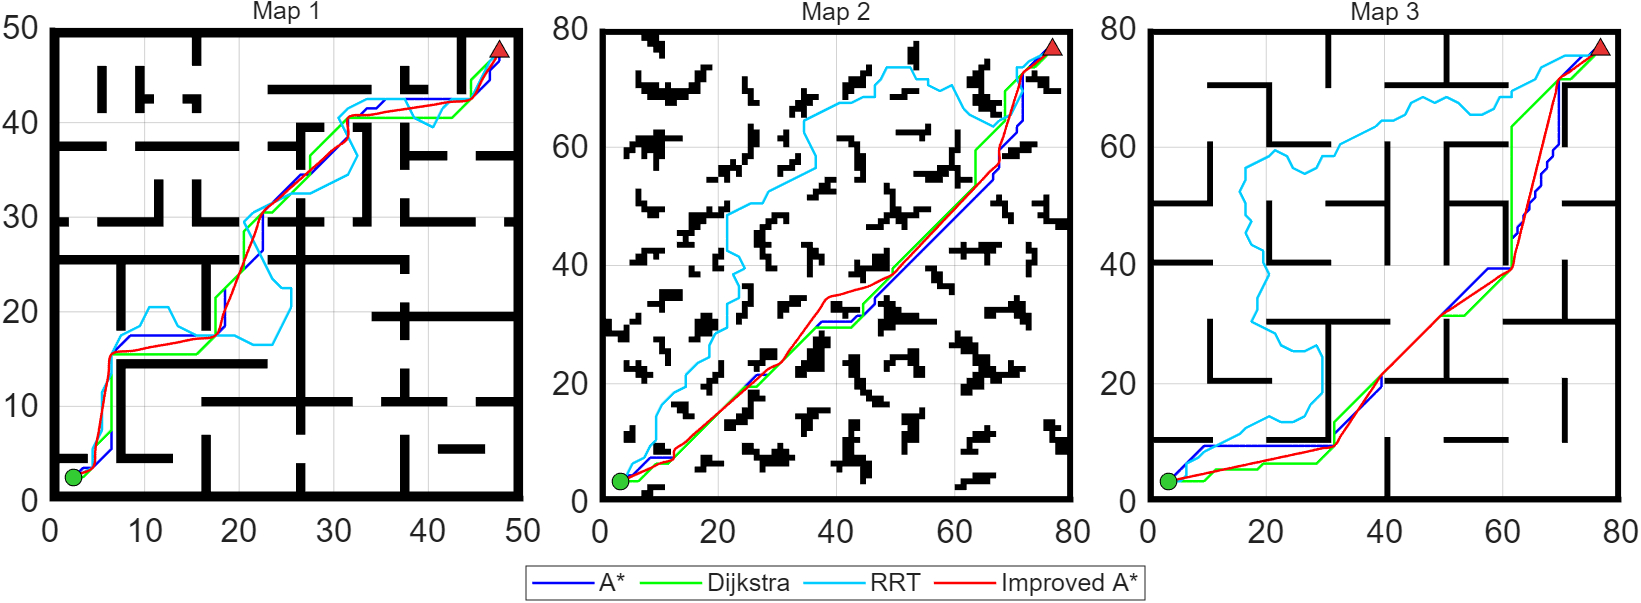
\includegraphics[width=0.92\textwidth]{figures/DifPathPlan_pathCompare}
\caption{Path-planning results of the four algorithms on the three maps.}
\label{fig:plan_paths}
\end{figure*}

\begin{figure}[!ht]
\centering
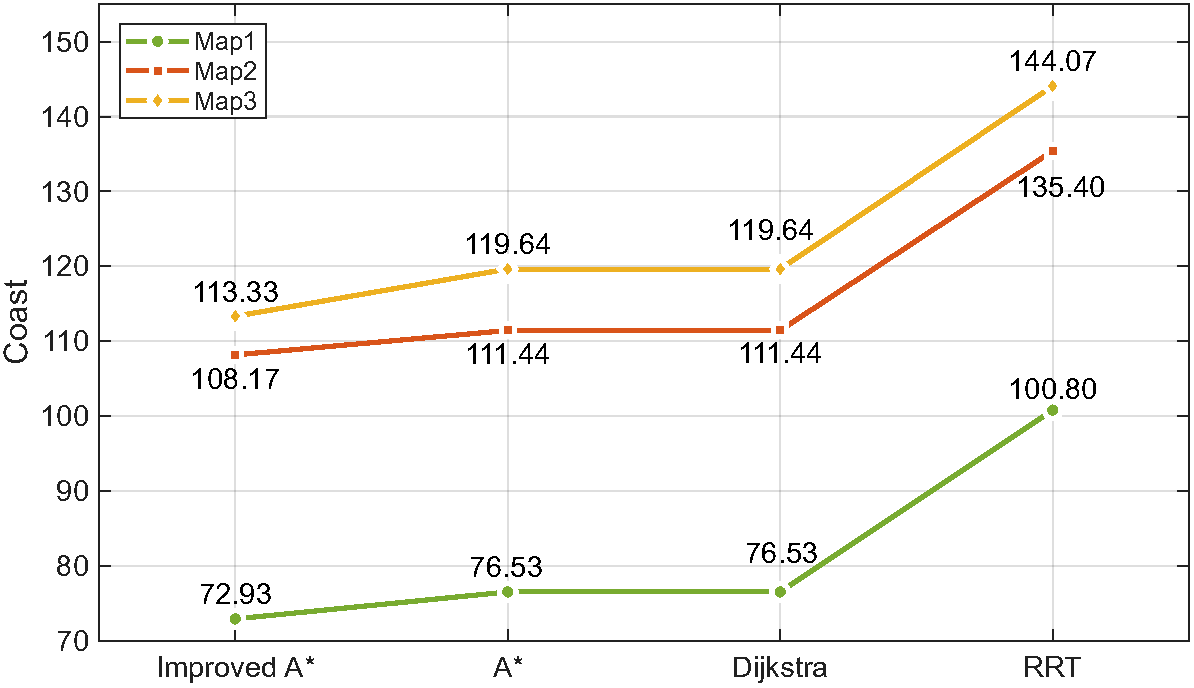
\includegraphics[width=2.5in]{figures/DifPathPlan_CostCompare}
\caption{Path-length comparison of the four algorithms on Map~1, 2, and 3.}
\label{fig:plan_len}
\end{figure}
\begin{figure}[!ht]
\centering
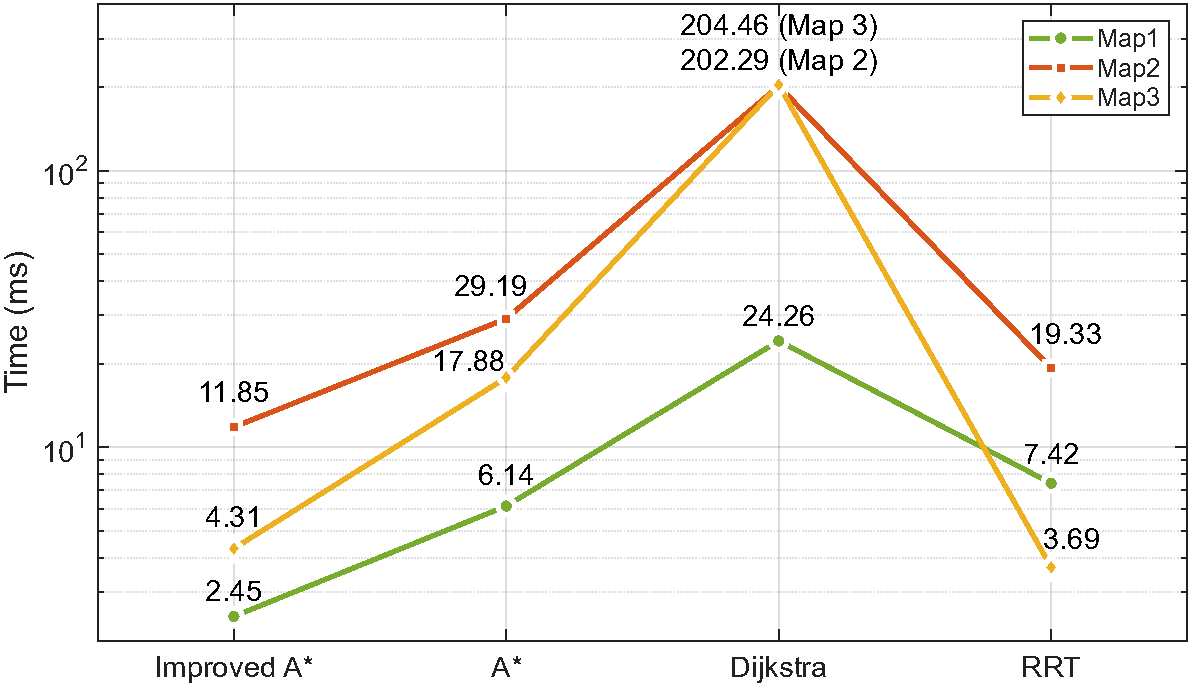
\includegraphics[width=2.5in]{figures/DifPathPlan_TimeCompare}
\caption{Computation-time comparison of the four algorithms on Map~1, 2, and 3.}
\label{fig:plan_time}
\end{figure}

We first consider path length. Table~\textcolor{blue}{\ref{tab:plan}} shows that the proposed method achieves 72.93, 108.17, and 113.33 on Map~1--Map~3, respectively, which are approximately 4.7\%, 2.9\%, and 5.3\% shorter than those of conventional A* and Dijkstra. The line trends in Fig.~\textcolor{blue}{\ref{fig:plan_len}} are consistent with the table, indicating that the advantage is not an isolated coincidence. It should be noted that, under an admissible heuristic, conventional A* and Dijkstra produce the optimal polyline in the grid metric; the fact that their lengths coincide confirms that both have reached the discrete optimum. The shorter length of the proposed method is mainly not because ``another shorter grid path was found,'' but because post-processing turns the staircase-like polyline into a more compact continuous trajectory: safety-aware simplification merges redundant waypoints and trims detours around corners, and spline smoothing further removes jaggedness, bringing the result closer to the physically continuous shortest travel. In other words, the length advantage corresponds directly to the simplification--smoothing mechanism of Section~\textcolor{blue}{\ref{subsec:post}}.

Next, we examine search efficiency. In terms of the number of expanded nodes, the proposed method is far below the two graph-search baselines on all three maps: relative to A*, the reductions are approximately 91.4\%, 79.0\%, and 98.3\%, respectively, and relative to Dijkstra the reduction exceeds about 92\% in every case. This phenomenon can be explained by the symmetry pruning of JPS: jump points are generated only at forced neighbors and at changes of direction, intermediate same-direction cells are no longer inserted into the open set one by one, and the search tree is therefore greatly compressed. On the same map, Dijkstra expands uniformly in all directions, and conventional A*, although guided by a heuristic, still relaxes cell by cell; hence the expanded-node counts differ by an order of magnitude. At the same time, it should be noted objectively that the reduction relative to A* on Map~2 is noticeably smaller than on Map~1 and Map~3: fragmented obstacles make forced neighbors more frequent, the number of jump points rises, and the pruning benefit is partially offset. Even so, an order-of-magnitude advantage over cell-by-cell expansion is maintained overall.

We further compare with sampling-based methods. RRT becomes the fastest method on Map~3 with 3.69~ms. This result must be reported honestly: when the maze corridors are regular and the start and goal are almost connected by a straight line, a random tree may find a feasible solution quickly. The price, however, is a marked degradation in path quality---the RRT path is the longest on all three maps, about 25\%--38\% longer than that of the proposed method. Moreover, as a randomized sampling method, its results fluctuate across runs, which is consistent with the typical weak sampling consistency of such methods. Therefore, under an evaluation protocol that requires both short paths and stable reproducibility, RRT does not constitute a substantive threat to the proposed method. If the task only requires a feasible solution quickly, sampling methods still have their applicable scope.

In summary, the three metrics corroborate one another. The length advantage comes from the approximation of continuous travel by simplification--smoothing, whereas the expansion and time advantages come from the pruning of the search tree by JPS. The two correspond to different mechanisms in the post-processing pipeline and the graph-search kernel, respectively. The relatively narrower pruning gain on Map~2 indicates that forced neighbors in highly cluttered grids weaken the symmetry benefit of JPS, yet both the expanded-node count and the computation time remain comprehensively better than those of cell-by-cell graph search. Future work may consider adaptively adjusting pruning or jump-point generation strategies on highly cluttered maps to further reduce the search overhead in such scenarios.

\begin{figure*}[!ht]
\centering
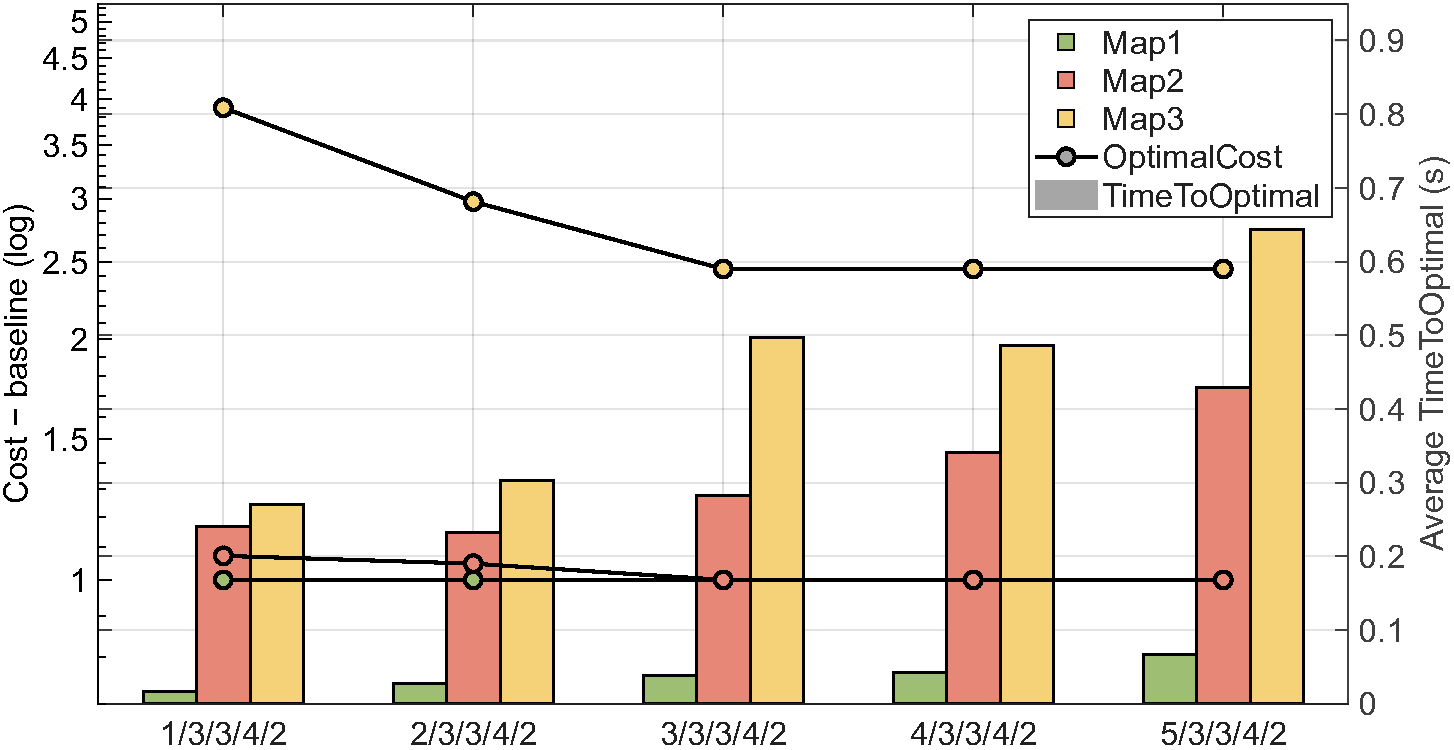
\includegraphics[width=0.32\textwidth]{figures/Sensitivity_Cost&Time_nAnts}\hfil
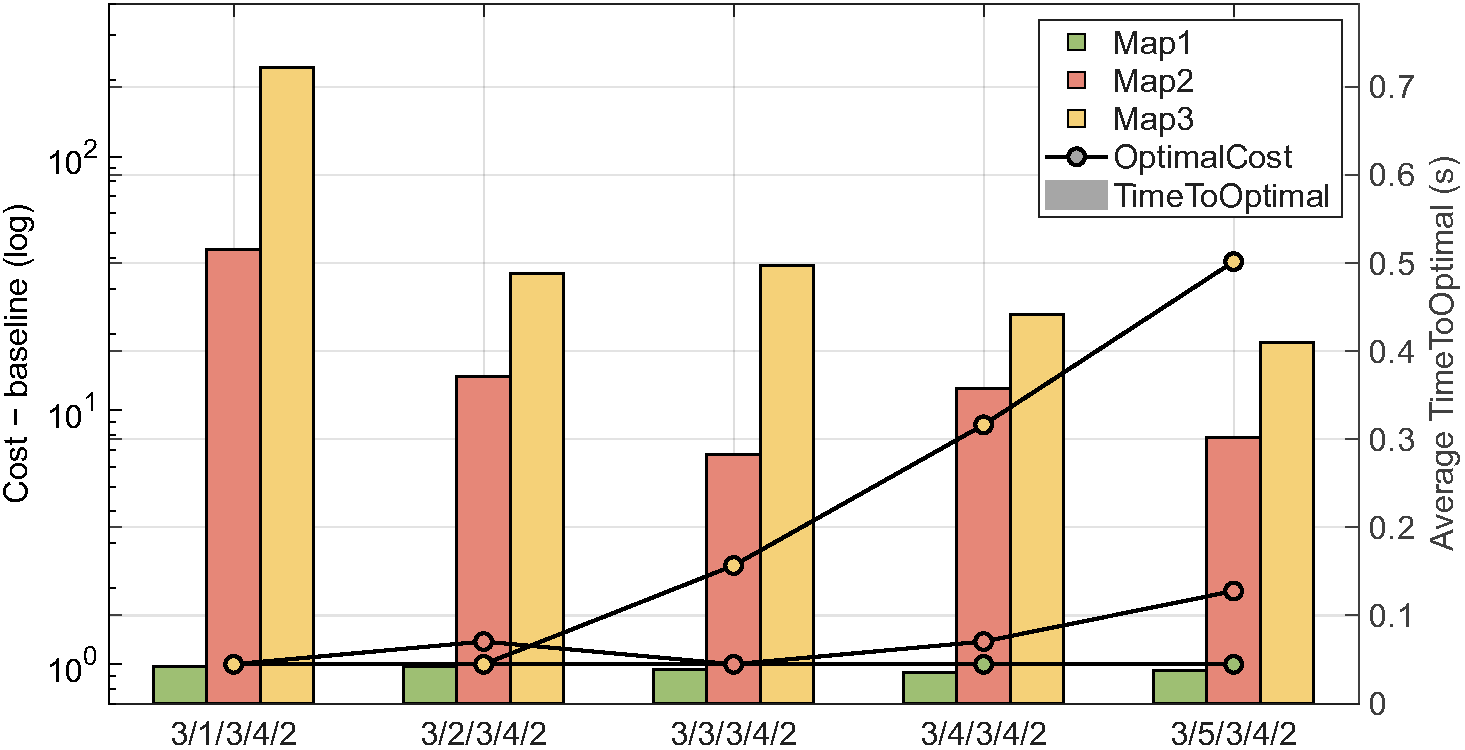
\includegraphics[width=0.32\textwidth]{figures/Sensitivity_Cost&Time_q0}\hfil
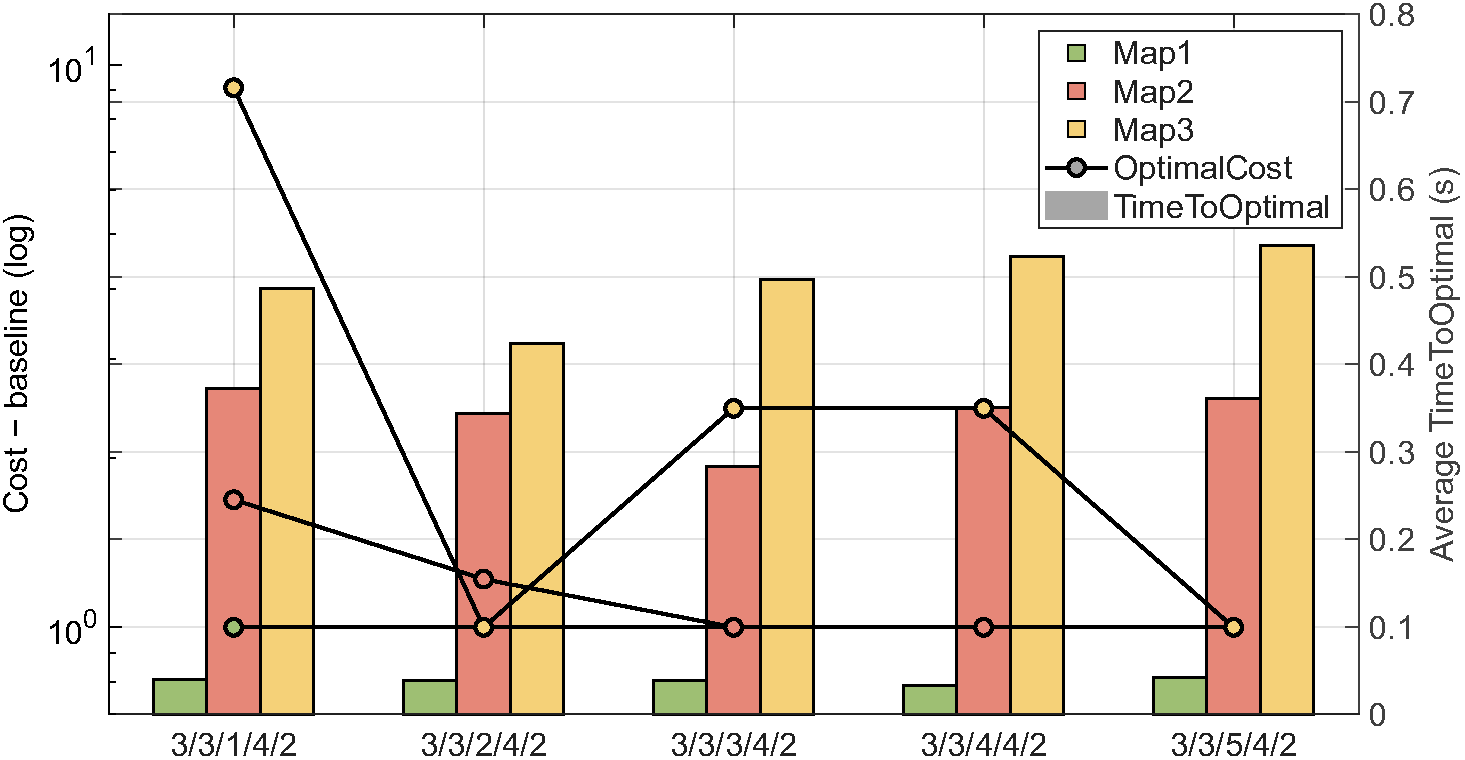
\includegraphics[width=0.32\textwidth]{figures/Sensitivity_Cost&Time_ymax}\\
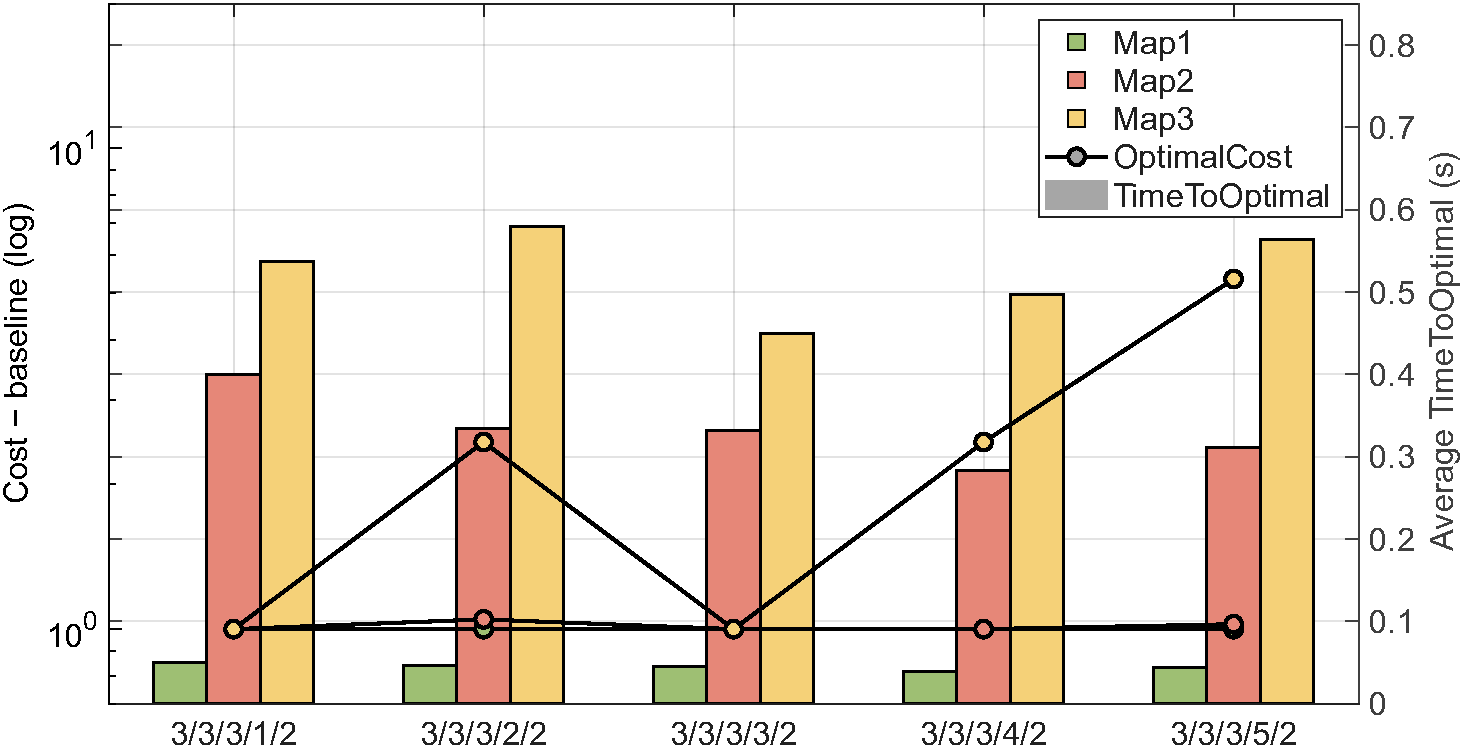
\includegraphics[width=0.32\textwidth]{figures/Sensitivity_Cost&Time_relite}\hfil
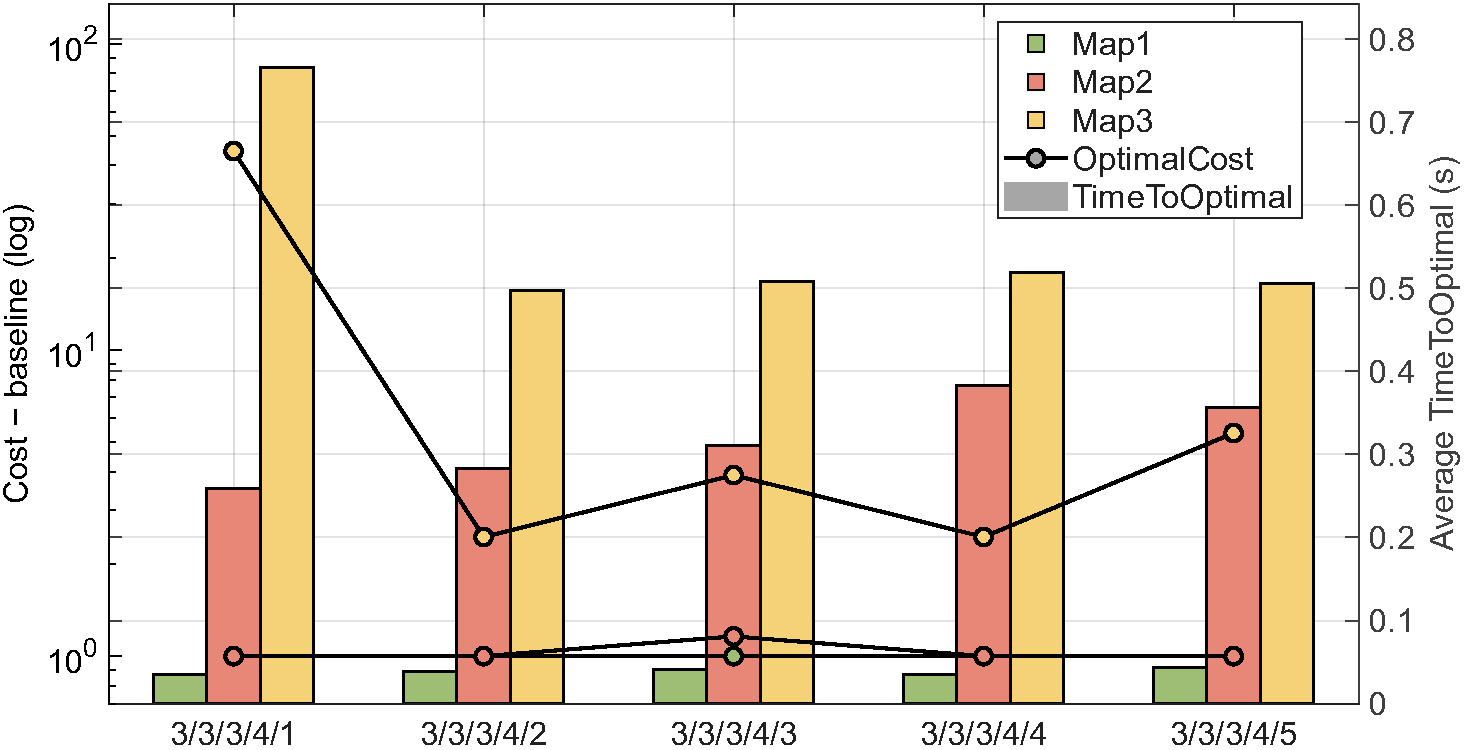
\includegraphics[width=0.32\textwidth]{figures/Sensitivity_Cost&Time_k}
\caption{Cost and computation time of each parameter level on Map~1, Map~2, and kroB100.}
\label{fig:sens_cost_time}
\end{figure*}

\subsection{Parameter Sensitivity Analysis}
\label{subsec:exp_sens}

This group of experiments examines the sensitivity of MMAS-VND-CL to five key hyperparameters, namely the number of ants $n_{\mathrm{ants}}$, the greedy selection probability $q_0$, the late-stage local-search ratio $y_{\max}$, the elite ratio $r_{\mathrm{elite}}$, and the candidate-list size $k$. Five parameter levels are first defined for each of these five parameters, as shown in Table~\textcolor{blue}{\ref{tab:levels}}. The level settings of subsequent experimental groups are denoted by the combined form $n_{\mathrm{ants}}/q_0/y_{\max}/r_{\mathrm{elite}}/k$. A single-factor design is adopted in the experiments: only one parameter is varied over its five levels at a time, while the remaining parameters are kept at their defaults. A total of 21 single-factor configurations are implemented, among which the experimental groups 3/3/3/4/2 correspond to the default parameter-level combination. Each group is run independently 40 times on Map~1, Map~2, and kroB100. Evaluation considers not only the best cost, but also the mean cost with standard deviation and the average convergence time. The cost--time trends are shown in Fig.~\textcolor{blue}{\ref{fig:sens_cost_time}}, and the path morphology under the default parameters is shown in Fig.~\textcolor{blue}{\ref{fig:sens_paths}}.

\begin{table}[!t]
\caption{Parameter Levels Used in the Sensitivity Analysis}
\label{tab:levels}
\centering
\setlength{\tabcolsep}{4pt}
\begin{tabular}{lccccc}
\toprule
\multirow{2}{*}{Parameter} & \multicolumn{5}{c}{Parameter Levels} \\
\cmidrule(lr){2-6}
 & Level 1 & Level 2 & Level 3 & Level 4 & Level 5 \\
\midrule
$n_{\mathrm{ants}}$ & 10 & 20 & \textbf{40} & 60 & 90 \\
$q_0$ & 0.10 & 0.30 & \textbf{0.45} & 0.60 & 0.90 \\
$y_{\max}$ & 0.10 & 0.20 & \textbf{0.40} & 0.60 & 0.90 \\
$r_{\mathrm{elite}}$ & 0.1 & 0.3 & 0.5 & \textbf{0.7} & 0.9 \\
$k$ & 3 & \textbf{9} & 15 & 30 & 60 \\
\bottomrule
\end{tabular}
\end{table}

\begin{figure}[!ht]
\centering
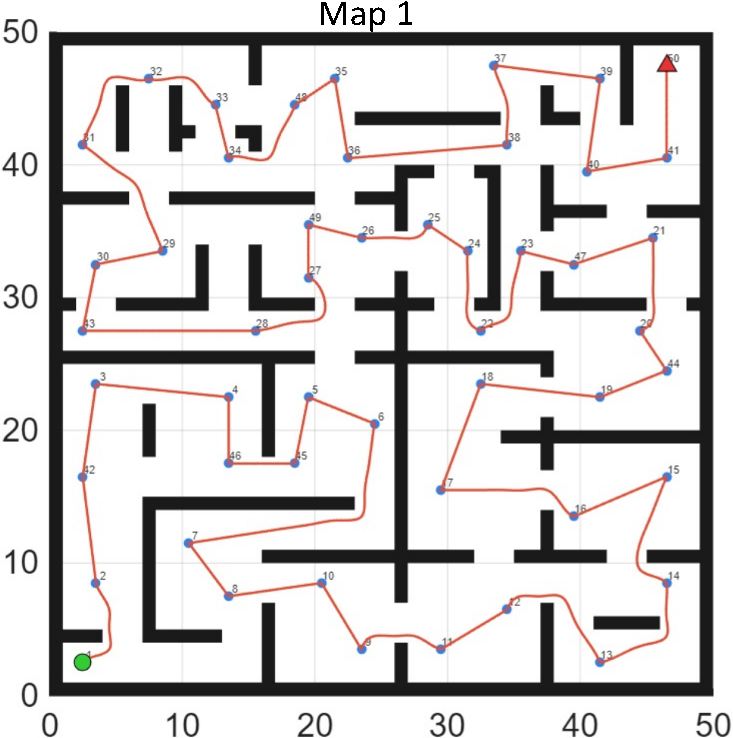
\includegraphics[width=1.55in]{figures/DifTSP_path_Map1_My}\hfil
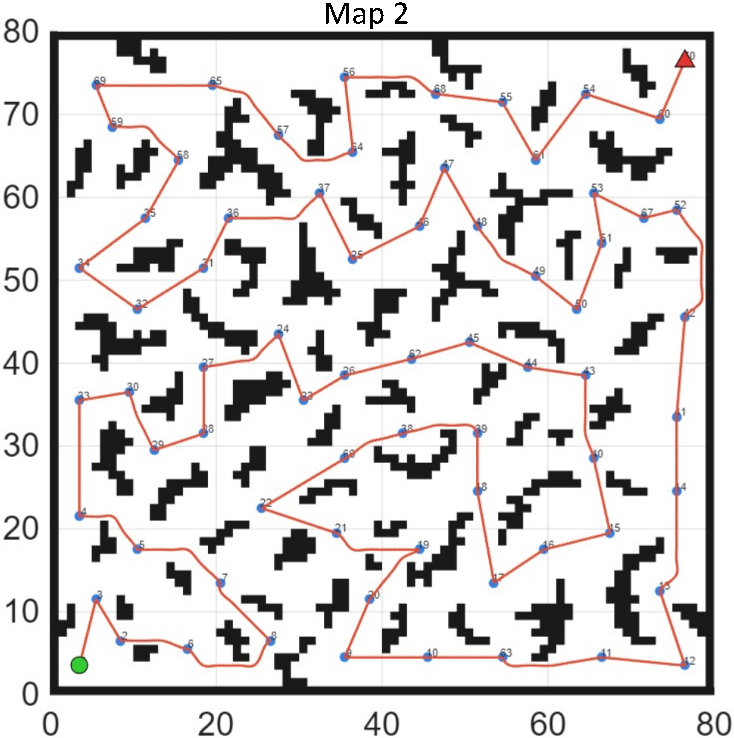
\includegraphics[width=1.55in]{figures/DifTSP_path_Map2_My}\\
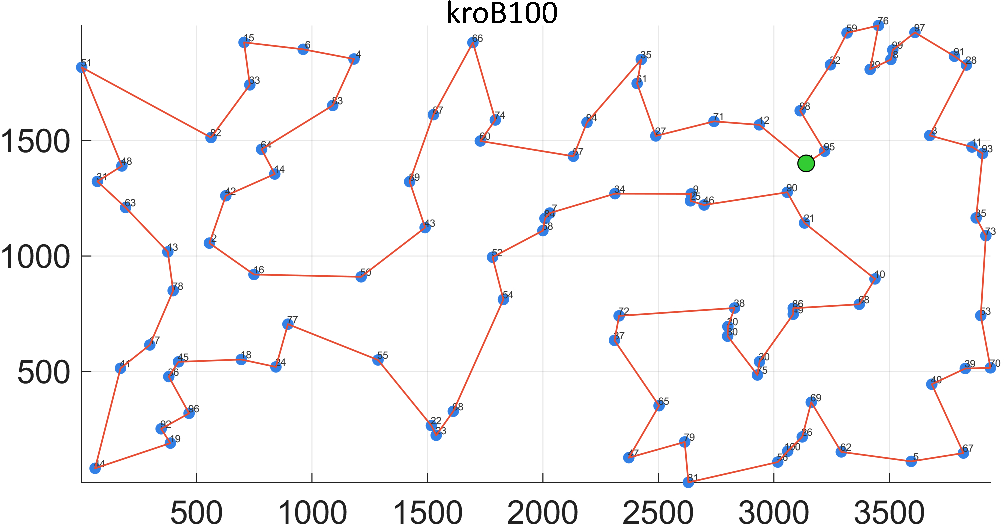
\includegraphics[width=2.5in]{figures/DifTSP_path_kroB100_My}
\caption{Paths planned by the algorithm on Map~1, Map~2, and kroB100 under the default parameter settings.}
\label{fig:sens_paths}
\end{figure}

For Map~1, Map~2, and kroB100, the reference best costs are 352.56, 623.78, and 22141, respectively. From the perspective of the reference best cost, the sensitivity results in the experimental data show that all configurations are able to reach the same reference value. This indicates that MMAS-VND-CL has a strong ability to ``find a high-quality solution'' within a reasonable parameter range; what truly separates the configurations is the mean cost and the computation time. Combining these observations with Fig.~\textcolor{blue}{\ref{fig:sens_cost_time}}, the main conclusions are as follows: $q_0$ and $y_{\max}$ are the most sensitive, $n_{\mathrm{ants}}$ and $r_{\mathrm{elite}}$ are intermediate, and $k$ is relatively flat within a moderate range but collapses when it is too small. The default combination ($3/3/3/4/2$) strikes a relatively balanced trade-off among quality, stability, and time, and is therefore fixed for subsequent experiments. The parameters are discussed individually below.

In terms of parameter regularity, the parameter $q_0$ controls the balance between exploitation and exploration in the pseudo-random transition. When it is set to 0.90 (nearly pure greedy), the ant colony almost always locks onto the currently highest-scoring candidate, and the pheromone rapidly collapses onto a small number of edges: the success rate on kroB100 drops to 57.5\% with the standard deviation rising to 45.78, and Map~2 reaches only 70\%. Lowering $q_0$ to 0.10--0.30 preserves a 100\% success rate, but the computation time becomes noticeably longer (about 490--720~ms). The parameter $y_{\max}$ determines the intensity of late-stage VND refinement. At $y_{\max}=0.10$, the lack of intensified late-stage local search leaves the success rate on Map~2 at only 62.5\%. At $y_{\max}=0.90$, the success rate instead declines, presumably because overly strong local search prematurely locks some runs into suboptimal structures.

Increasing $n_{\mathrm{ants}}$ from 10 to 40 raises the success rate on Map~2 from 92.5\% to 100\% and that on kroB100 from 95\% to 97.5\%. When the population is too small, pheromone updates are easily biased by a few individuals and the variance increases. Further increasing $n_{\mathrm{ants}}$ to 60--90 no longer improves the success rate, while the computation time increases by about 20\%--60\%; this is a ``sufficient and inexpensive'' compromise. When $r_{\mathrm{elite}}$ is set to 0.1--0.5, the success rate on kroB100 can reach 100\% or nearly 100\%, whereas over-elitization at 0.9 reduces it to 92.5\%. Over the range 9--60, $k$ has little effect on the cost, but at $k=3$ candidate pruning filters out promising edge exchanges as well, the success rate falls to 42.5\%, and the computation time rises to about 765.9~ms.

It should also be pointed out that no single configuration dominates on every metric; evaluation must trade off hit quality, stability, and computation time. The default combination, with values $40/0.45/0.40/0.7/9$, achieves a 100\% hit rate with zero variance on Map~1 and Map~2, and on kroB100 attains a 97.5\% success rate with a relatively small standard deviation in about 500~ms. Its overall performance is the most balanced, and therefore the subsequent ablation and algorithm-comparison experiments all adopt this configuration.


\subsection{Ant Colony Optimization Component Ablation}
\label{subsec:exp_ablation}

\begin{table}[!t]
\caption{Ablation experiment groups}
\label{tab:ablation_groups}
\centering
\small
\setlength{\tabcolsep}{4pt}
\begin{tabular}{cll}
\toprule
Group & Description & Disabled Mechanism \\
\midrule
1 & Complete Algorithm & None \\
2 & No Pseudo-Random & ACS Pseudo-Random Transfer Rule \\
3 & No VND & VND Local Search \\
4 & No S-Curve & Progressive Local Search Scheduling \\
5 & No Candidate List & Candidate List Acceleration \\
6 & No MMAS & MMAS Pheromone Boundary \\
\bottomrule
\end{tabular}
\end{table}

\begin{figure}[!t]
\centering
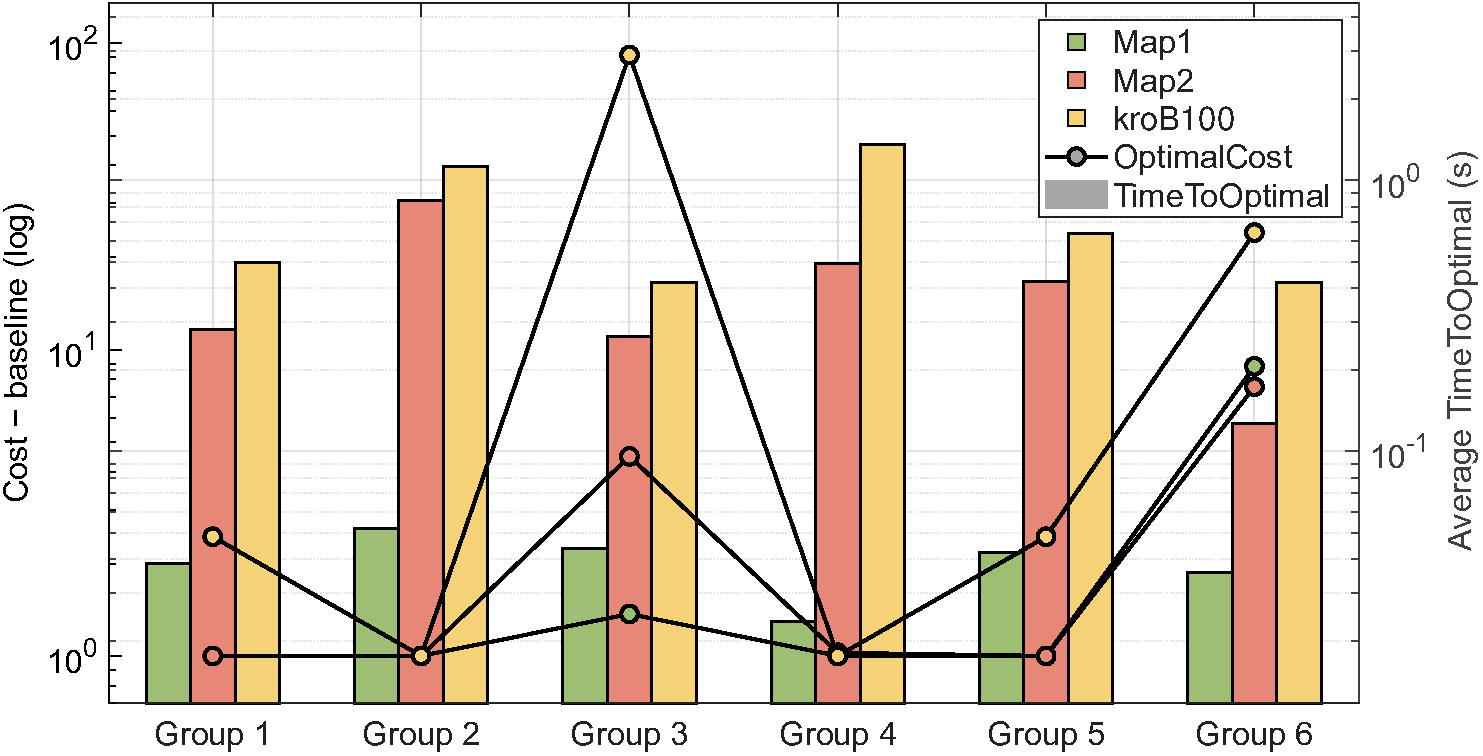
\includegraphics[width=3in]{figures/Ablation_Cost&Time}
\caption{Comparison of mean cost and mean computation time of the six ablation groups on the three maps.}
\label{fig:abl_cost_time}
\end{figure}

\begin{table}[!t]
\caption{Ablation experiment results}
\label{tab:ablation}
\centering
\footnotesize
\setlength{\tabcolsep}{2.5pt}
\begin{tabular}{cccccc}
\toprule
Map & Group & Best cost & \makecell{Path\\Mean/std.dev} & \makecell{Run Time\\(ms)} & \makecell{Success rate\\(\%)} \\
\midrule
 \multirow{6}{*}{Map 1} & 1 & \textbf{352.56} & \textbf{352.56}/\textbf{0.00} & 38.6 & \textbf{100} \\
   & 2 & \textbf{352.56} & \textbf{352.56}/\textbf{0.00} & 51.9 & \textbf{100} \\
   & 3 & \textbf{352.56} & 352.93/0.75 & 43.9 & 80 \\
   & 4 & \textbf{352.56} & \textbf{352.56}/\textbf{0.00} & \textbf{23.5} & \textbf{100} \\
   & 5 & \textbf{352.56} & \textbf{352.56}/\textbf{0.00} & 42.2 & \textbf{100} \\
   & 6 & \textbf{352.56} & 360.39/13.81 & 35.7 & 52.5 \\
\midrule
 \multirow{6}{*}{Map 2} & 1 & \textbf{623.78} & \textbf{623.78}/\textbf{0.00} & 282.9 & \textbf{100} \\
   & 2 & \textbf{623.78} & \textbf{623.78}/\textbf{0.00} & 846.4 & \textbf{100} \\
   & 3 & \textbf{623.78} & 627.26/2.53 & 265.2 & 10 \\
   & 4 & \textbf{623.78} & 623.80/0.15 & 492.9 & 97.5 \\
   & 5 & \textbf{623.78} & \textbf{623.78}/\textbf{0.00} & 422.2 & \textbf{100} \\
   & 6 & \textbf{623.78} & 630.34/6.47 & \textbf{126.8} & 10 \\
\midrule
 \multirow{6}{*}{kroB100} & 1 & \textbf{22141.00} & 22142.45/9.17 & 496.7 & 97.5 \\
   & 2 & \textbf{22141.00} & \textbf{22141.00}/\textbf{0.00} & 1126.3 & \textbf{100} \\
   & 3 & \textbf{22141.00} & 22231.50/73.36 & \textbf{419.9} & 12.5 \\
   & 4 & \textbf{22141.00} & 22141.00/0 & 1357.6 & \textbf{100} \\
   & 5 & \textbf{22141.00} & 22142.45/9.17 & 637.1 & 97.5 \\
   & 6 & \textbf{22141.00} & 22164.10/41.74 & \textbf{419.9} & 72.5 \\
\bottomrule
\end{tabular}
\end{table}

To isolate the independent contribution of each mechanism in MMAS-VND-CL, this experiment disables one mechanism at a time while keeping all other settings unchanged, yielding six groups as listed in Table~\textcolor{blue}{\ref{tab:ablation_groups}}. Each group is run 40 times on Map~1, Map~2, and kroB100. The joint evaluation remains the best cost, mean cost/standard deviation, run time, and success rate; the overall results are summarized in Table~\textcolor{blue}{\ref{tab:ablation}}. The mean cost and mean computation time of each group are compared in Fig.~\textcolor{blue}{\ref{fig:abl_cost_time}}. The overall conclusion is as follows: VND and the MMAS pheromone bounds jointly determine whether a good solution can be obtained reliably, and neither is dispensable; pseudo-random transfer, the S-curve schedule, and the candidate list mainly govern how quickly a good solution is obtained, with relatively limited marginal effects on solution quality but decisive effects on computational cost. It should be noted in advance that the mean cost of some ablation groups still approaches that of the complete algorithm, and they are even faster in some cases. Such apparently better outcomes do not contradict the hierarchy above; they are explained below in terms of the underlying mechanisms.

We first examine VND (Group~3). Disabling local search markedly degrades solution quality: the mean cost rises on all three maps, from 352.56 to 352.93 on Map~1, from 623.78 to 627.26 on Map~2, and from 22142.45 to 22231.50 on kroB100; the standard deviation expands accordingly, from 9.17 to 73.36 on kroB100, and the stability across runs drops markedly. This behavior is consistent with the intended mechanism: pheromone guidance during construction can yield a reasonably ordered tour, whereas VND is the key step for effectively optimizing path quality. Without it, the population merely wanders around coarser solutions, and both the mean cost and the variance rise.

The second component is the MMAS pheromone boundary (Group~6). Removing the dynamic $\tau_{\min}$/$\tau_{\max}$ clipping reduces the success rates on Map~1 and Map~2 to 52.5\% and 10\%, respectively, and that on kroB100 to 72.5\%, while both the mean cost and the standard deviation deteriorate noticeably. The reason is that, without boundary constraints, pheromone on early favored edges can grow without limit, the search quickly locks onto a few path structures, and typical premature convergence occurs; multiple runs fall into different suboptimal basins, hence the pattern of occasionally touching the optimum but failing in most trials. A noteworthy exception is that Group~6 is not slow on any of the three maps, and is even the fastest on Map~2. This does not indicate a faster algorithm; rather, premature homogenization of the population triggers the adaptive stopping criterion earlier and reduces ineffective iterations, trading reliability for an apparent speed advantage.

We next consider the two components that primarily affect efficiency. Removing pseudo-random transfer (Group~2) leaves the success rate on all three maps no lower than that of the complete algorithm, but the run time rises to nearly two to three times that of the full method. This shows that the value of controlled greediness lies in accelerating convergence and saving the search budget, corroborating the observation in Section~\textcolor{blue}{\ref{subsec:exp_sens}} that a lower $q_0$ is more stable but slower. Removing the S-curve schedule (Group~4), i.e., applying local search at the maximum intensity from the first iteration, still yields a 100\% success rate on kroB100, but the run time increases by about 1.7$\times$; on Map~1 the run time is in fact the shortest. These results suggest that fixed high-intensity local search need not be disadvantageous on small instances, but can rapidly exhaust the computational budget on medium and large ones. The S-curve schedule defers refinement to the second half of the iteration precisely to balance early exploration against late-stage refinement. Removing the candidate list (Group~5) leaves solution quality almost unchanged while increasing the run time, consistent with its design goal of preserving neighborhood optimality while merely reducing ineffective evaluations.

In summary, VND determines whether the optimum can be approached reliably, and the MMAS boundary determines whether the population locks in prematurely; together they form the two pillars of solution quality. Pseudo-random transfer, the S-curve schedule, and the candidate list mainly regulate the convergence rate and computational overhead. The complete algorithm attains a 100\% hit rate on Map~1 and Map~2, and a 97.5\% success rate with small variance on kroB100 in about 500~ms, representing a balanced operating point in quality, stability, and time. All subsequent algorithm comparison experiments therefore adopt the complete configuration of Group~1. If an application places greater weight on absolute success rate, the proportion of late-stage local search can be increased or the stagnation limit extended.

\subsection{Multi-Goal Traversal Comparison of Different TSP Solvers}
\label{subsec:exp_cmp}

\begin{table}[!t]
\caption{Parameter settings of the compared TSP solvers}
\label{tab:tsp_params}
\centering
\scriptsize
\begin{tabular}{>{\centering\arraybackslash}m{0.22\columnwidth} m{0.68\columnwidth}}
\toprule
Algorithm & Main parameters \\
\midrule
MMAS-VND-CL & $n_{\mathrm{ants}}=40$;
$\alpha=1$;
$\beta=2$;\newline
$\rho=0.25$;
$Q=225$;
$\tau_0=0.1$;\newline
$q_0=0.45$;
$y_{\max}=0.4$;\newline
$r_{\mathrm{elite}}=0.7$;
$k=9$ \newline
Local search transition interval$=[0,30]$;\\
\midrule
ACO & $n_{\mathrm{ants}}=40$;
$\alpha=1$;
$\beta=2$;
$\rho=0.25$;\newline
$Q=225$;
$\tau_0=0.1$;
$\mathrm{Iter}=100$ \\
\midrule
GA & $\mathrm{Pop}=100$;
$\mathrm{Iter}=1500$;\newline
$P_c=0.8$;
$P_m=0.25$;\newline
Number of elites$=10$ \\
\midrule
SA & $T_0=150$;
$\alpha=0.996$;\newline
$L=10$;
$T_{\mathrm{end}}=10^{-8}$ \\
\bottomrule
\end{tabular}
\end{table}

\begin{table}[!t]
\caption{Multi-goal traversal comparison results}
\label{tab:tsp_cmp}
\centering
\scriptsize
\setlength{\tabcolsep}{2.5pt}
\begin{tabular}{cccccc}
\toprule
Map & Algorithm & Best cost & \makecell{Path\\Mean/std.dev} & \makecell{Run Time\\(ms)} & \makecell{Success rate\\(\%)} \\
\midrule
 \multirow{4}{*}{Map 1} & MMAS-VND-CL & \textbf{352.56} & \textbf{352.56}/\textbf{0.00} & \textbf{38.6} & \textbf{100} \\
   & ACO & 361.41 & 391.53/18.44 & 90.6 & 0 \\
   & GA & 411.07 & 496.28/46.93 & 4181.1 & 0 \\
   & SA & 365.13 & 413.82/25.83 & 784.6 & 0 \\
\midrule
 \multirow{4}{*}{Map 2} & MMAS-VND-CL & \textbf{623.78} & \textbf{623.78}/\textbf{0.00} & 241.5 & \textbf{100} \\
   & ACO & 641.09 & 691.64/18.61 & \textbf{223.2} & 0 \\
   & GA & 710.83 & 868.79/66.45 & 6693.6 & 0 \\
   & SA & 655.71 & 687.25/13.02 & 506.3 & 0 \\
\midrule
 \multirow{4}{*}{kroB100} & MMAS-VND-CL & \textbf{22141.00} & \textbf{22142.45}/\textbf{9.17} & \textbf{496.7} & \textbf{97.5} \\
   & ACO & 23153.00 & 24546.05/606.87 & 534.1 & 0 \\
   & GA & 32243.00 & 36772.55/2894.73 & 8817.2 & 0 \\
   & SA & 23487.00 & 24871.05/753.20 & 516.5 & 0 \\
\bottomrule
\end{tabular}
\end{table}

\begin{figure*}[!htbp]
\centering
\subfloat[Map~1]{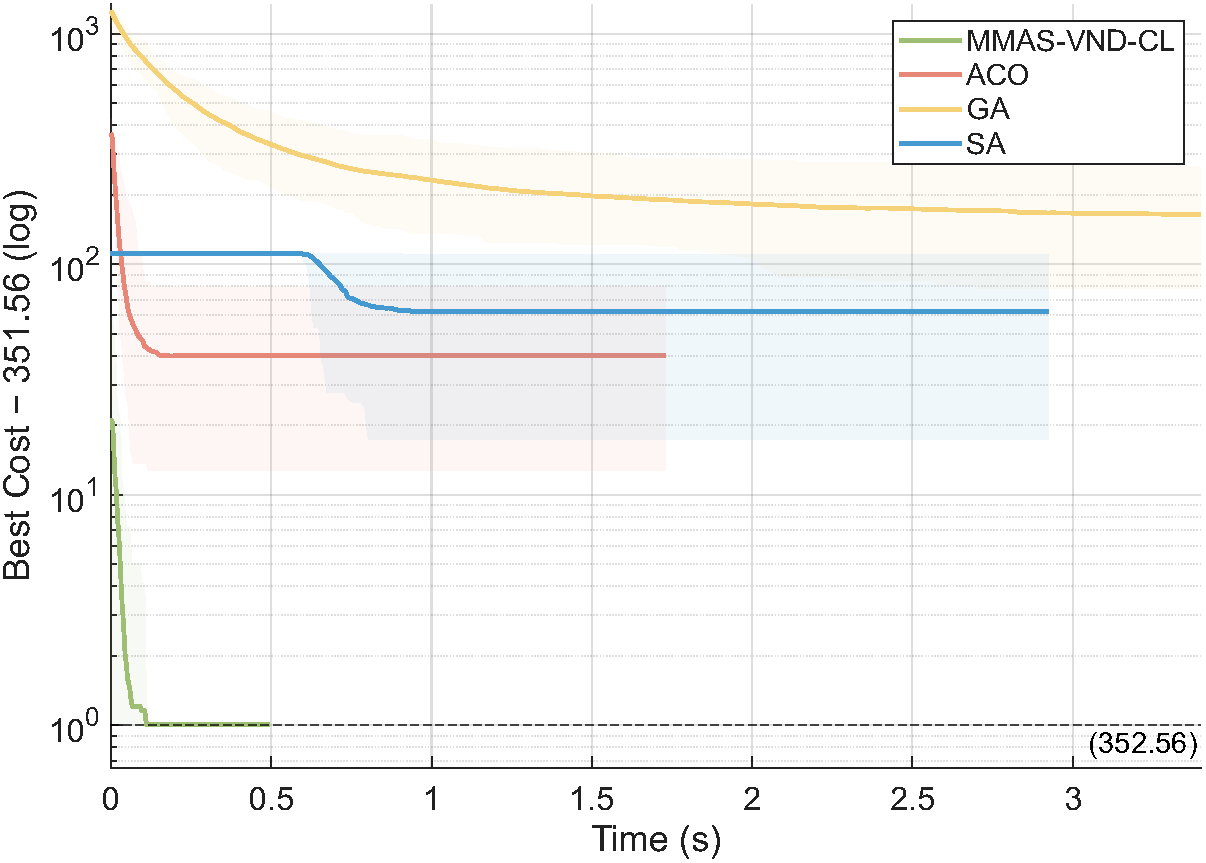
\includegraphics[width=0.3\textwidth]{figures/DifTSP_Map1_conv}}\hfil
\subfloat[Map~2]{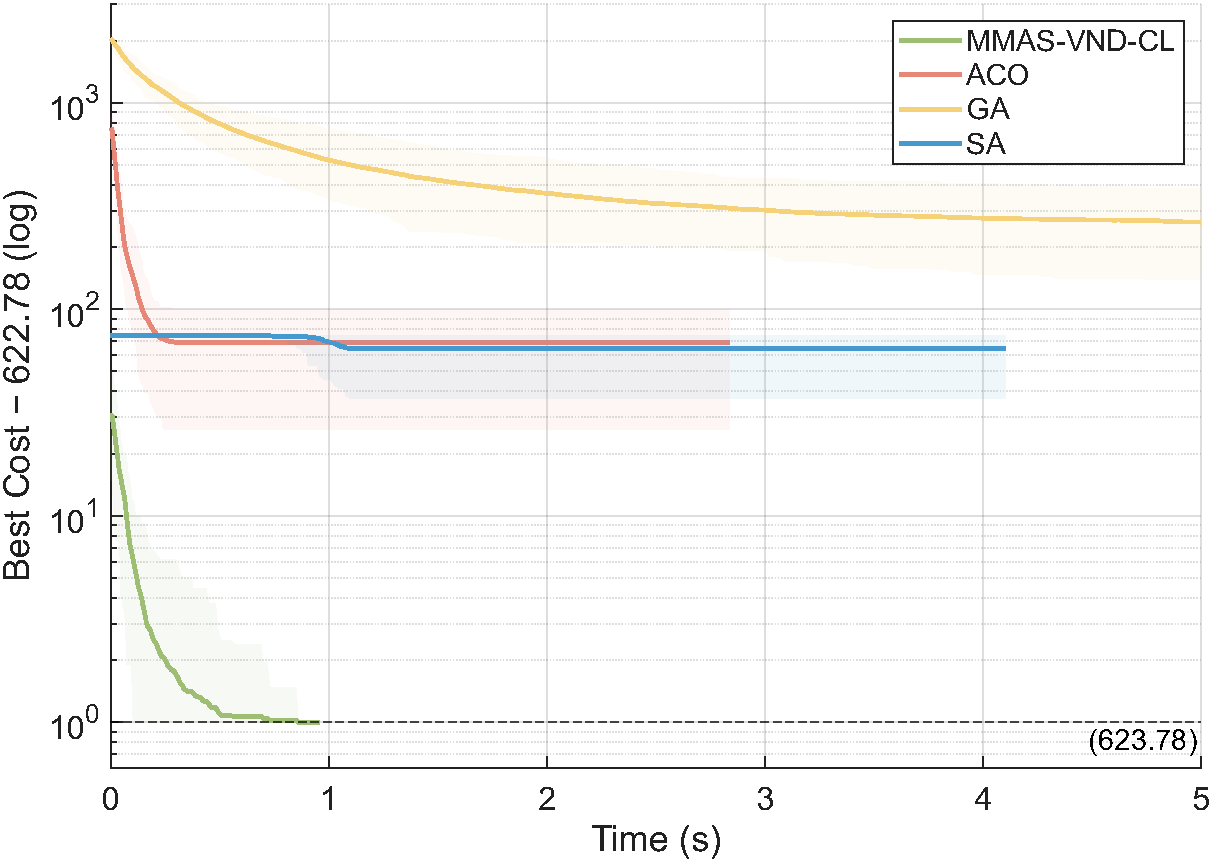
\includegraphics[width=0.3\textwidth]{figures/DifTSP_Map2_conv}}\hfil
\subfloat[kroB100]{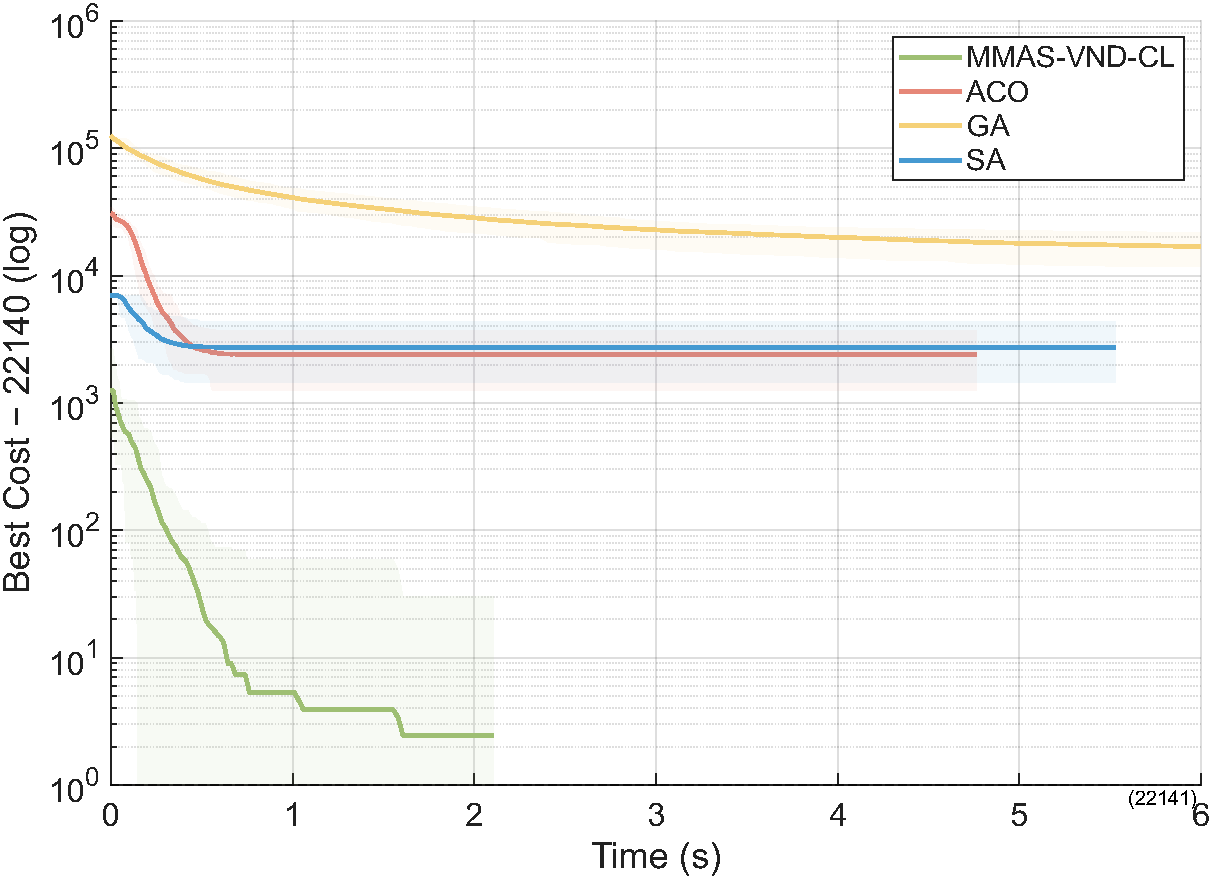
\includegraphics[width=0.3\textwidth]{figures/DifTSP_kroB100_conv}}
\caption{Mean time--cost convergence curves of the four TSP solvers over 40 runs on the three maps.}
\label{fig:tsp_conv}
\end{figure*}

\begin{figure*}[!htbp]
\centering
\subfloat[Map~1]{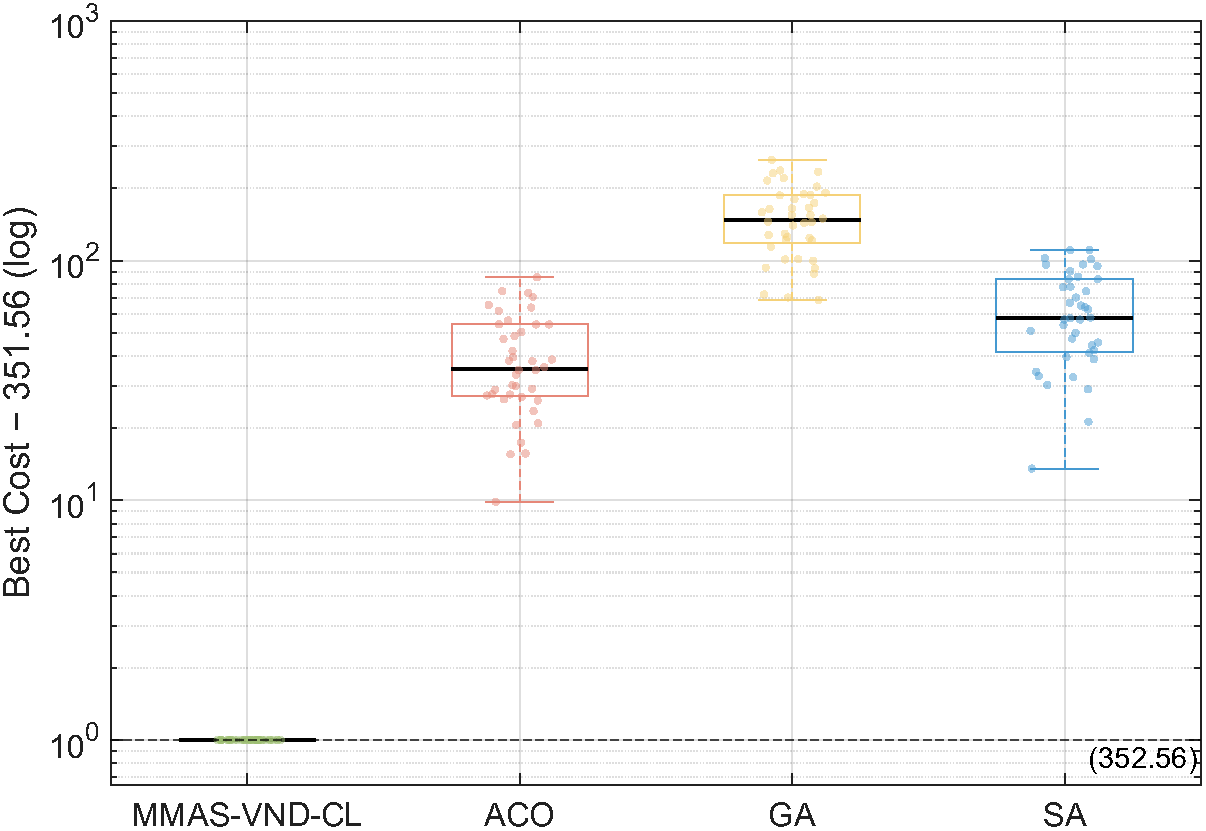
\includegraphics[width=0.3\textwidth]{figures/DifTSP_Map1_box}}\hfil
\subfloat[Map~2]{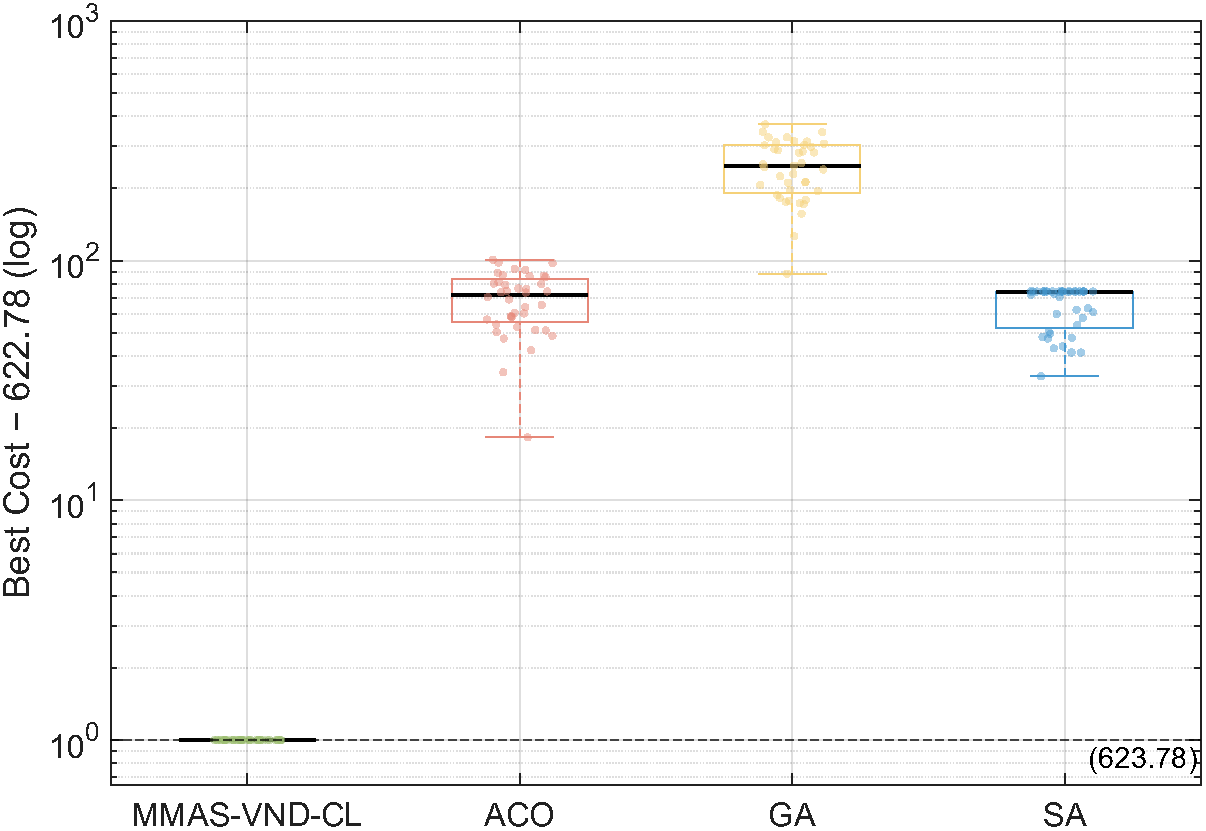
\includegraphics[width=0.3\textwidth]{figures/DifTSP_Map2_box}}\hfil
\subfloat[kroB100]{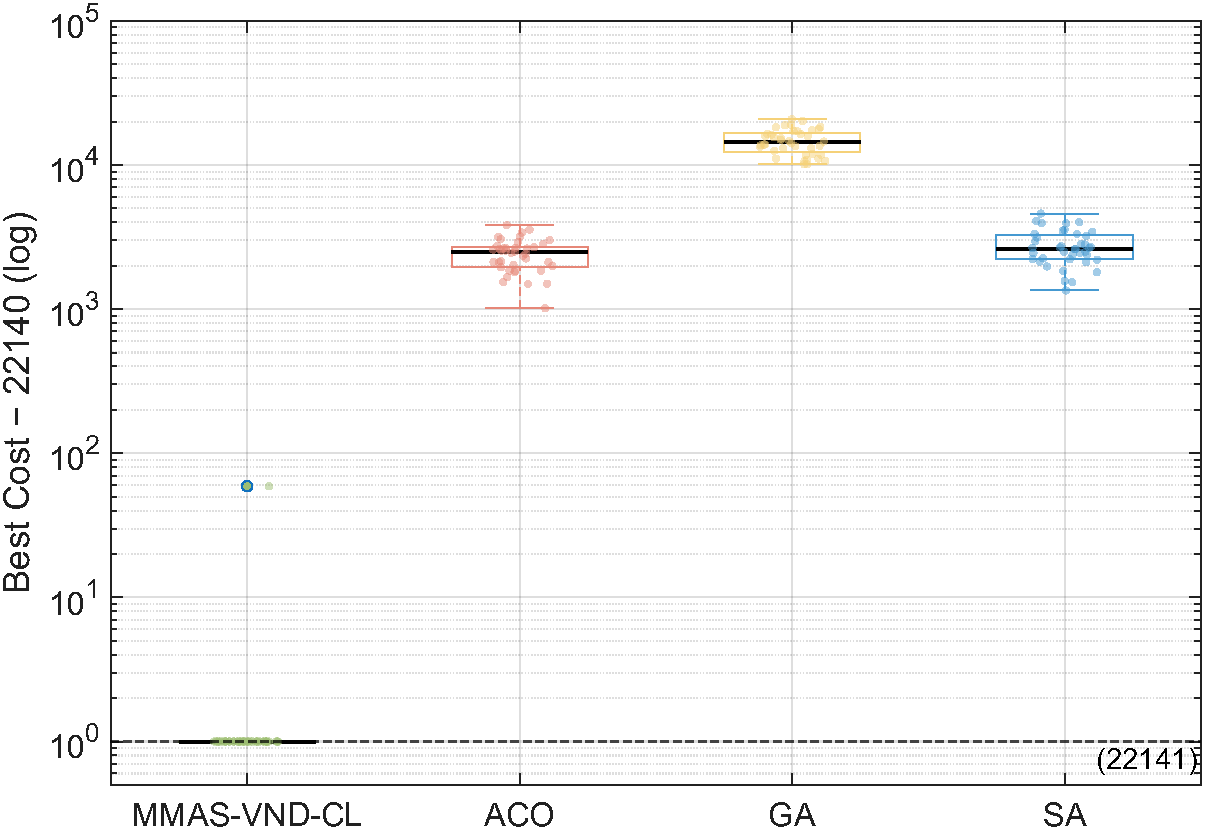
\includegraphics[width=0.3\textwidth]{figures/DifTSP_kroB100_box}}
\caption{Cost distributions of the four TSP solvers over 40 runs on the three maps.}
\label{fig:tsp_box}
\end{figure*}

With the front-end improved A* cost matrix and the virtual-node open encoding held fixed, this experiment replaces only the back-end TSP solver so as to examine the practical contribution of the sequencing module within the complete multi-goal traversal framework. Four solvers are compared: the proposed MMAS-VND-CL, a standard ant colony system (ACO), a genetic algorithm (GA), and simulated annealing (SA), with parameters given in Table~\textcolor{blue}{\ref{tab:tsp_params}}. Each combination is independently run 40 times on Map~1, Map~2, and kroB100. The conclusions can be summarized as follows: under the unified geometric cost interface and the tested parameter configurations, MMAS-VND-CL outperforms the three baseline metaheuristic implementations in solution quality, success rate, and stability, and its run time is also low in most settings. Only the lightweight ACO is slightly faster on Map~2, albeit with a clear gap in cost quality, whereas GA is clearly inferior in both quality and time. We elaborate below by metric--condition--mechanism, and discuss the individual cases that are faster but not better.

\begin{figure}[!htbp]
\centering
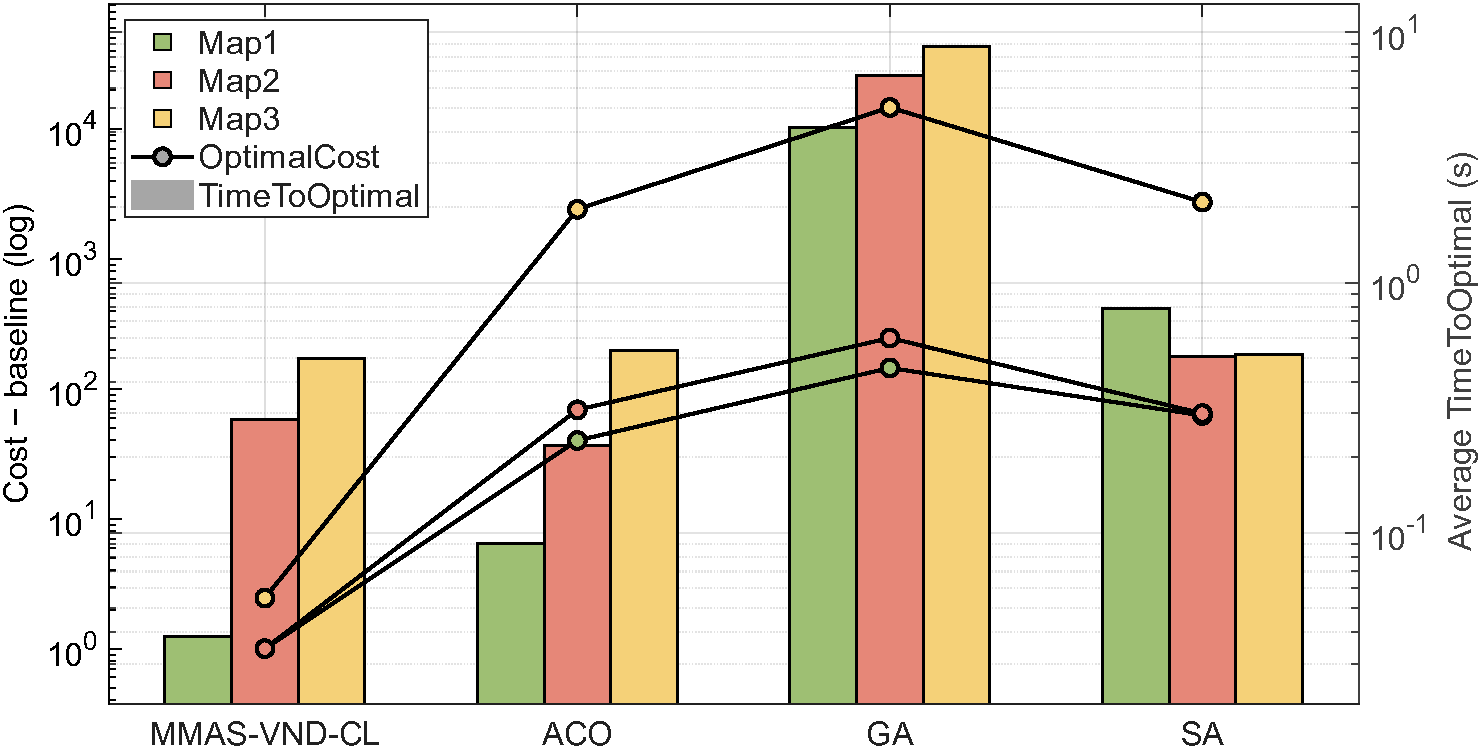
\includegraphics[width=3in]{figures/DifTSP_Map_Cost&Time}
\caption{Comparison of mean cost and mean computation time of the four TSP solvers on the three maps.}
\label{fig:tsp_cost_time}
\end{figure}

\begin{figure*}[!t]
\centering
\begin{minipage}[t]{0.48\textwidth}
\centering
\textbf{MMAS-VND-CL}\\[2pt]
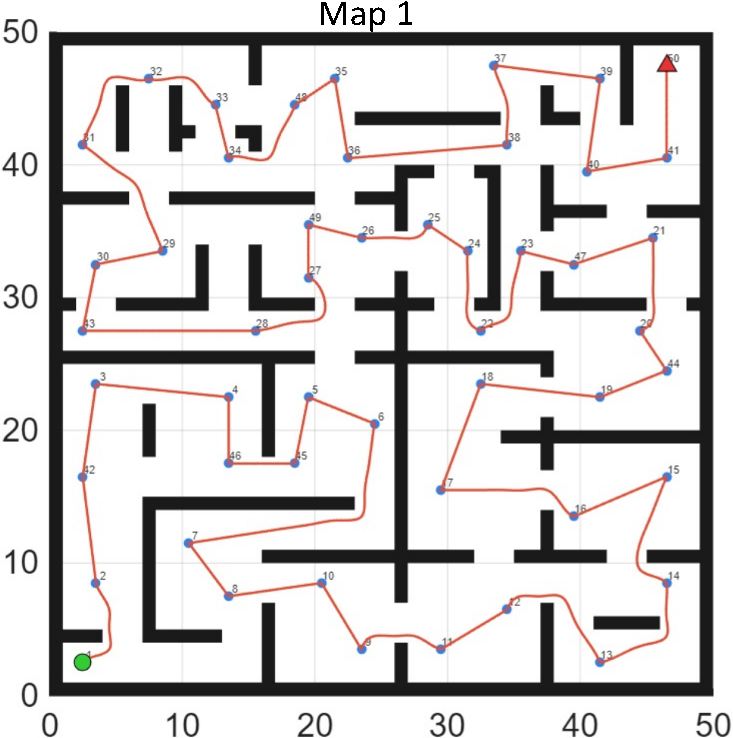
\includegraphics[width=0.46\linewidth]{figures/DifTSP_path_Map1_My}\hfil
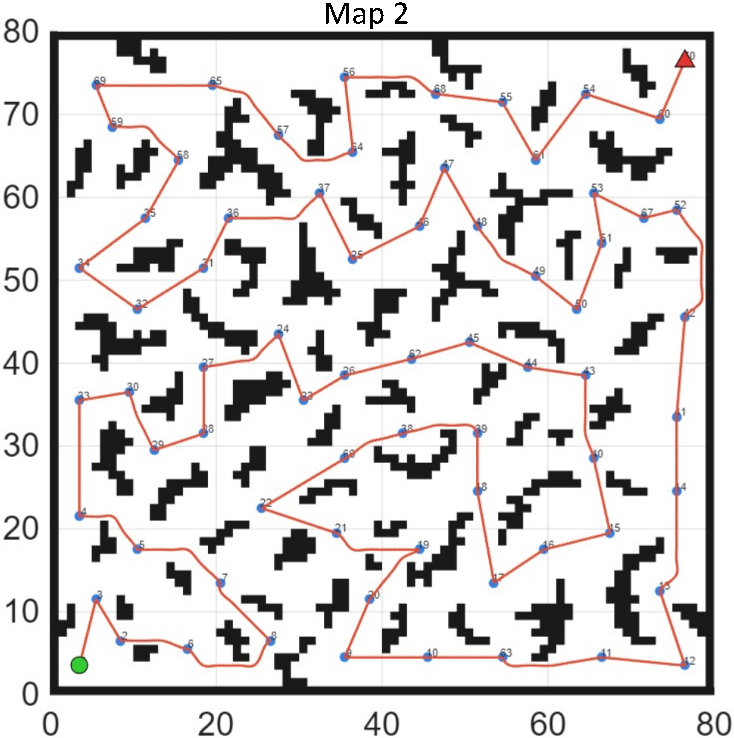
\includegraphics[width=0.46\linewidth]{figures/DifTSP_path_Map2_My}\\
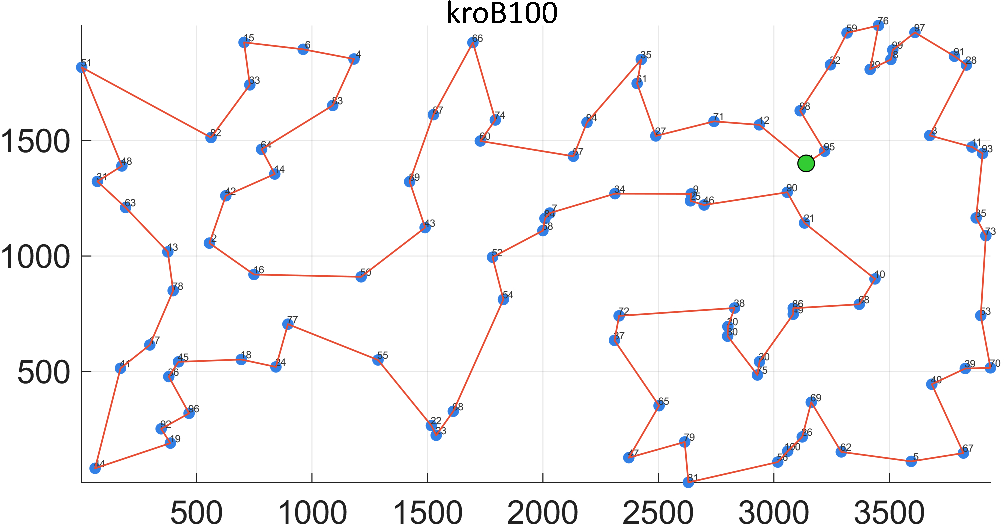
\includegraphics[width=0.78\linewidth]{figures/DifTSP_path_kroB100_My}
\end{minipage}\hfill
\begin{minipage}[t]{0.48\textwidth}
\centering
\textbf{ACO}\\[2pt]
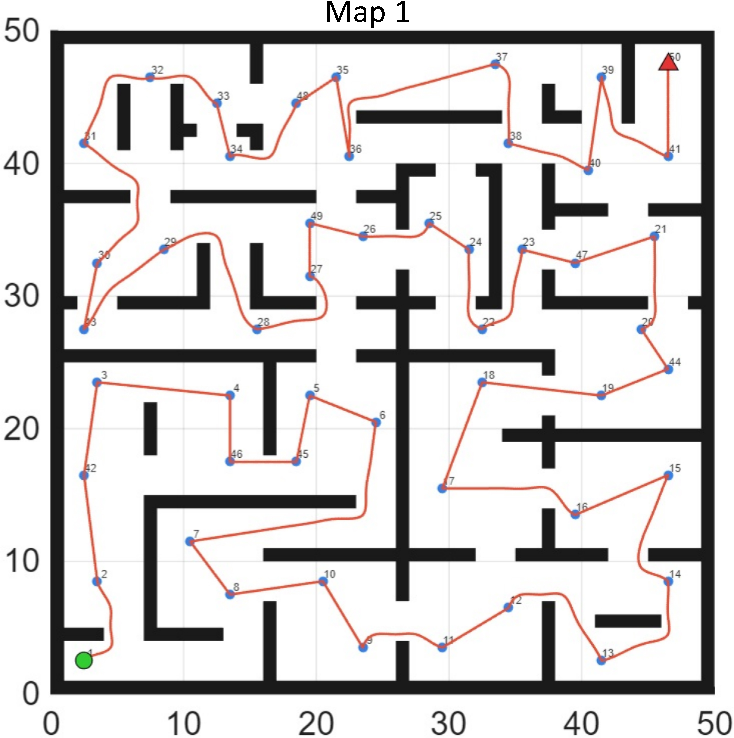
\includegraphics[width=0.46\linewidth]{figures/DifTSP_path_Map1_ACO}\hfil
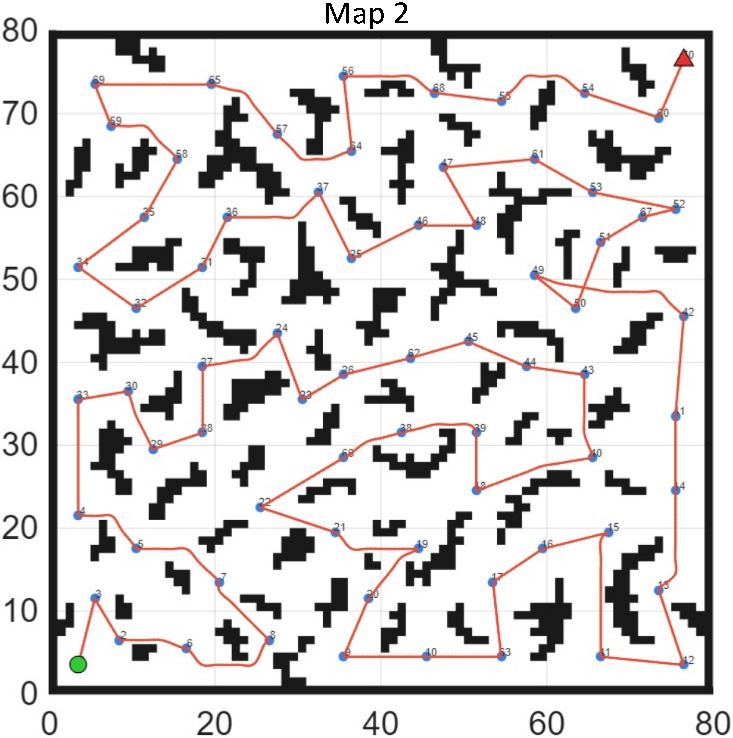
\includegraphics[width=0.46\linewidth]{figures/DifTSP_path_Map2_ACO}\\
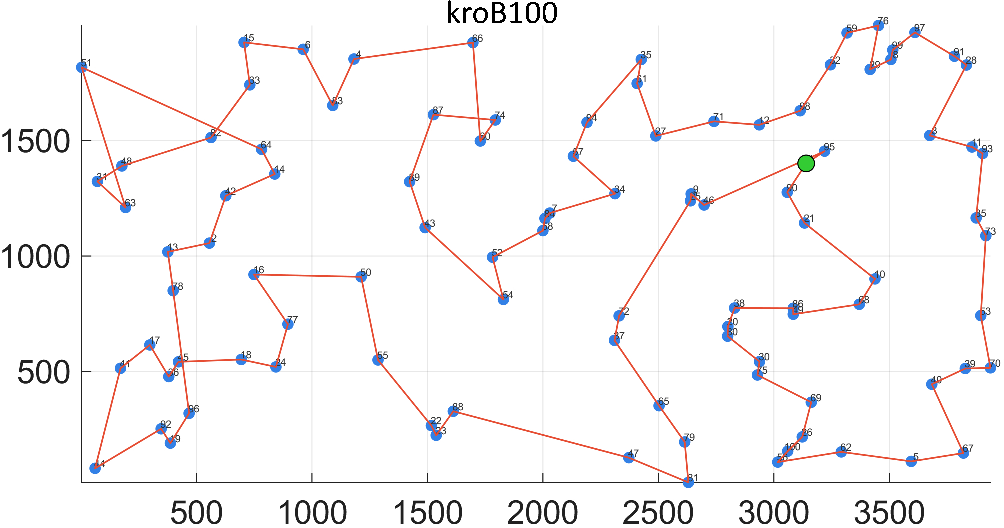
\includegraphics[width=0.78\linewidth]{figures/DifTSP_path_kroB100_ACO}
\end{minipage}

\vspace{8pt}

\begin{minipage}[t]{0.48\textwidth}
\centering
\textbf{GA}\\[2pt]
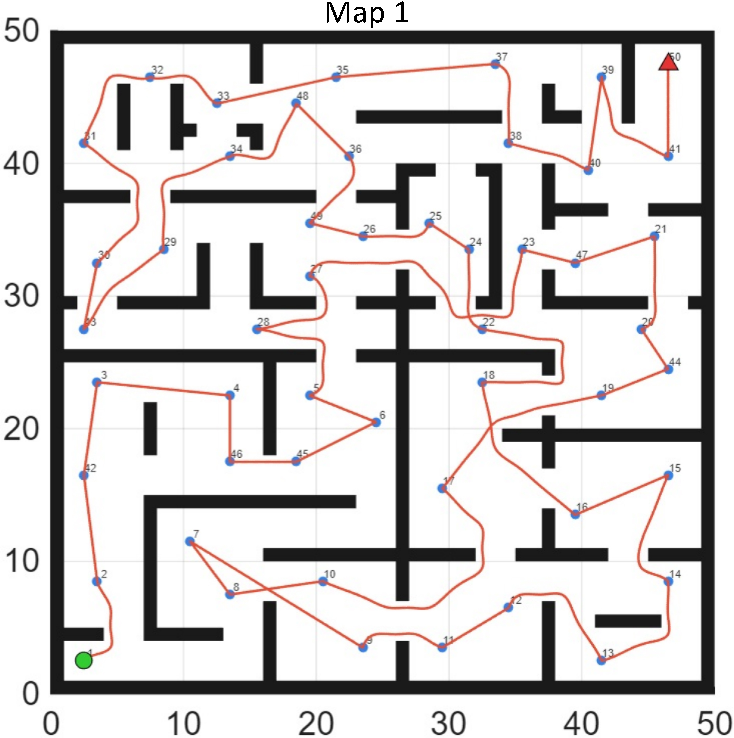
\includegraphics[width=0.46\linewidth]{figures/DifTSP_path_Map1_GA}\hfil
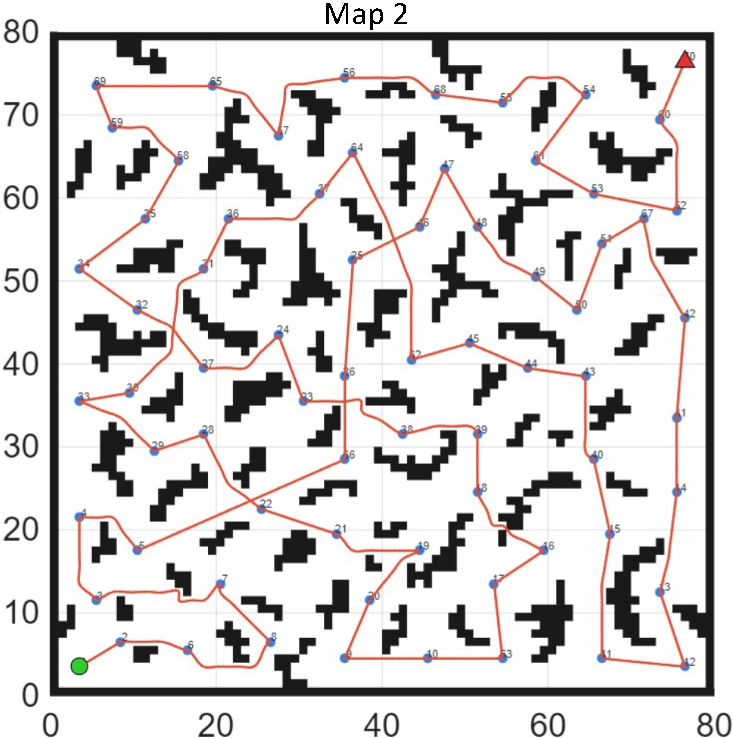
\includegraphics[width=0.46\linewidth]{figures/DifTSP_path_Map2_GA}\\
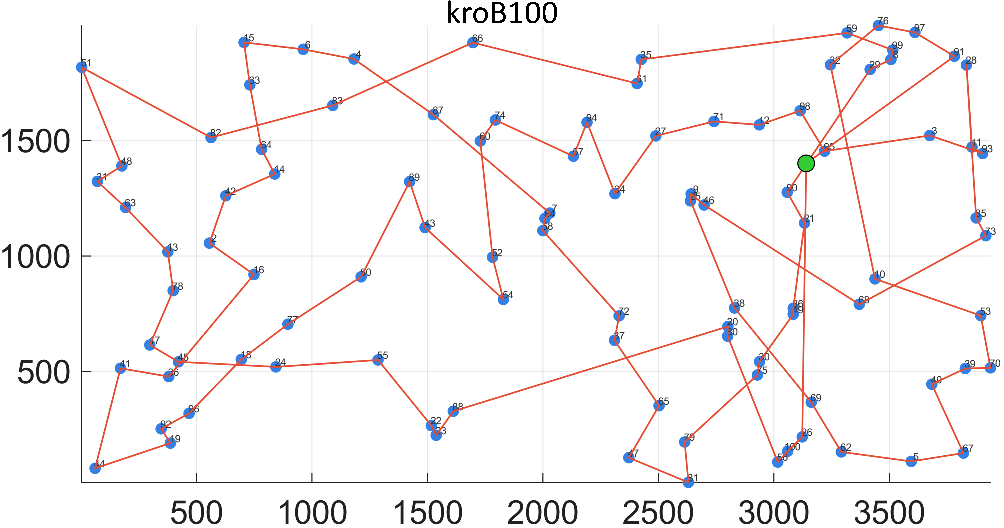
\includegraphics[width=0.78\linewidth]{figures/DifTSP_path_kroB100_GA}
\end{minipage}\hfill
\begin{minipage}[t]{0.48\textwidth}
\centering
\textbf{SA}\\[2pt]
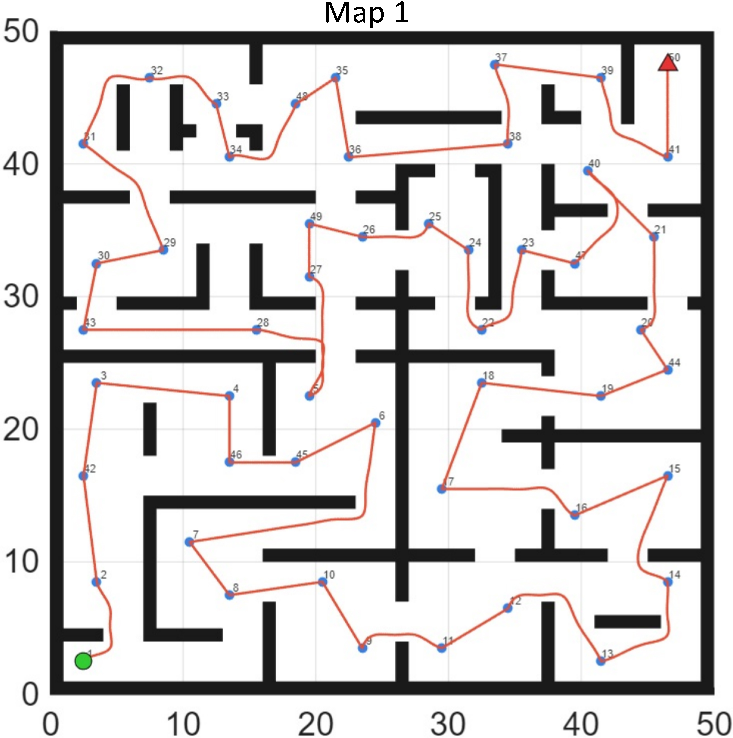
\includegraphics[width=0.46\linewidth]{figures/DifTSP_path_Map1_SA}\hfil
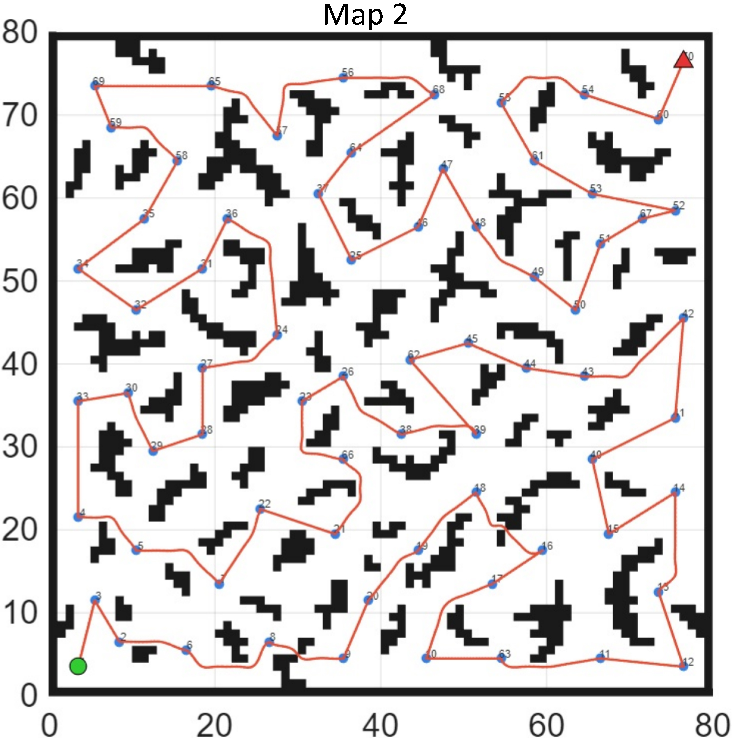
\includegraphics[width=0.46\linewidth]{figures/DifTSP_path_Map2_SA}\\
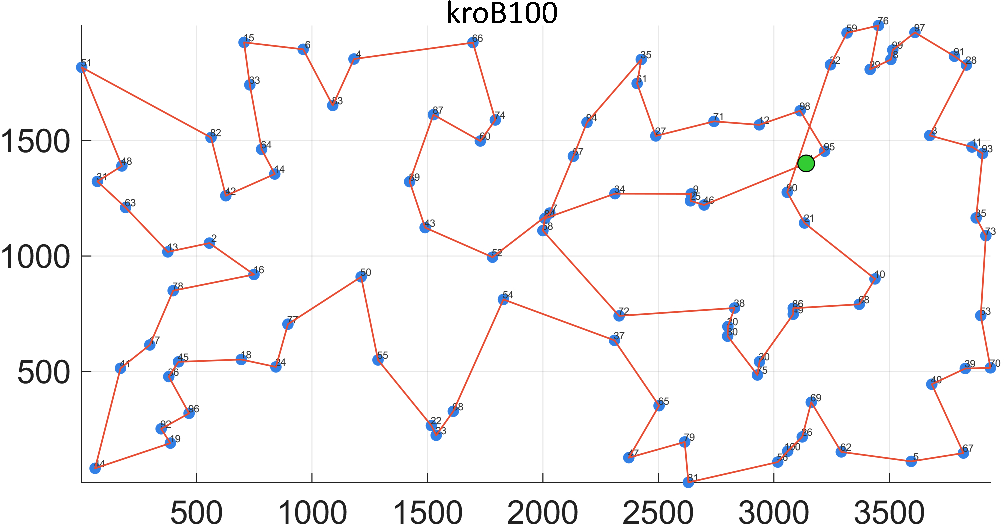
\includegraphics[width=0.78\linewidth]{figures/DifTSP_path_kroB100_SA}
\end{minipage}
\caption{Best-cost paths planned by each TSP solver on Map~1, Map~2, and kroB100.}
\label{fig:tsp_paths}
\end{figure*}

The multi-goal traversal performance of each solver is reported in Table~\textcolor{blue}{\ref{tab:tsp_cmp}}. The corresponding visualizations are shown in Figs.~\textcolor{blue}{\ref{fig:tsp_conv}}--\textcolor{blue}{\ref{fig:tsp_paths}}.

We first examine solution quality and success rate. Table~\textcolor{blue}{\ref{tab:tsp_cmp}} shows that MMAS-VND-CL attains the lowest best cost and mean cost on all three maps, and is the only solver that reliably reaches the reference optimum across repeated runs: all 40 runs reach the reference values 352.56 and 623.78 on Map~1 and Map~2, and on kroB100 the method reaches the reference value 22141 with a success rate of 97.5\% and a mean cost of 22142.45. The success rates of the other three algorithms are all 0\%, i.e., none of their 40 runs reaches the reference optimum. This does not mean that they fail to produce feasible solutions; the table shows mean costs ranging from 361.41 to 36772.55. The gap is most pronounced on kroB100: the mean cost of the compared ACO implementation is 24546.05, about 10.9\% higher than ours; SA is about 12.3\% higher; and GA, with a mean of 36772.55, is about 66\% higher. In Fig.~\textcolor{blue}{\ref{fig:tsp_paths}}, the baseline paths exhibit substantially more detours and crossings than the proposed method, and the boxes in Fig.~\textcolor{blue}{\ref{fig:tsp_box}} are longer with more dispersed whiskers, indicating that they are occasionally not too bad but systematically longer overall.

We next analyze algorithmic stability. On kroB100, the standard deviation of MMAS-VND-CL is only 9.17, whereas those of ACO, SA, and GA are 606.87, 753.20, and 2894.73, respectively, i.e., about 1.8 to 1.9 orders of magnitude smaller than ACO and SA and about 2.5 orders of magnitude smaller than GA. On Map~2, although SA has converged to 13.02, it is still higher than the zero variance of the proposed method. This can be understood from the mechanisms: the virtual-node encoding fixes the start and end nodes and includes them fully in pheromone updates; the MMAS bounds prevent early lock-in; and the candidate-list-accelerated VND performs aggressive refinement of elite tours in every generation. Together, these three factors suppress run-to-run fluctuation to a very low level. Standard ACO and SA, which lack VND and boundary control, can only rely on random perturbations during construction or neighborhood moves, so path quality scatters widely across initializations.

We then discuss time performance and offer an objective assessment with necessary concessions. In Table~\textcolor{blue}{\ref{tab:tsp_cmp}}, on Map~2 the ACO baseline is slightly faster than the proposed method, at 223.2~ms versus 241.5~ms, and is the only baseline that is superior in run time. The reason is straightforward: this baseline performs no large-scale VND neighborhood search, so each iteration is cheaper, whereas the proposed method spends part of its budget on local search and therefore has heavier iterations. On Map~1 and kroB100, however, the proposed method is faster: candidate-list pruning keeps the additional overhead of VND within a controllable range, whereas the baselines often require more iterations to reach comparable quality. GA falls behind on all counts: its run time on the three maps reaches several seconds while its cost remains the worst, indicating that its variable-length chromosome crossover lacks specificity for path-type representations and wastes search effort. Summarizing the time--cost trade-off in Fig.~\textcolor{blue}{\ref{fig:tsp_cost_time}}: the proposed method occupies the region of low cost and relatively low run time simultaneously, and on Map~2 it exchanges a negligible time difference for substantially better solution quality.

Finally, we provide mechanistic attribution and close the discussion. On the unified JPS cost matrix, the differences at the combination layer are isolated and amplified: the virtual-node open encoding ensures that the start and end constraints are not broken by the search; the MMAS pheromone bounds maintain diversity; ACS-style pseudo-random transfer accelerates convergence; the candidate-list VND drives the tour toward near-optimality; and the S-curve schedule together with adaptive stopping controls when and for whom refinement cost is paid. The experiments show that what truly separates the method from the baselines is the ability to reach the reference optimum reliably, rather than the best value of any single run. We also note the boundaries of the comparison conditions: the baselines use a single parameter set and a fixed iteration budget, without parameter searches comparable to those applied to the proposed method; the default parameters of the proposed method are selected by sensitivity analysis, with an iteration cap of 800 generations and additional VND local search. It should also be acknowledged that, if an application only requires a rapid feasible visit order, a lightweight ACO retains low-latency value in simple scenarios. If the number of goal points continues to grow, the computational share of VND will increase, and further strengthening of candidate-list compression or hierarchical local search will be needed. Considering quality, reliability, and computational overhead together, MMAS-VND-CL is better suited as the sequencing module for multi-goal traversal in obstacle environments under the tested configurations.

In addition to the simulated maps above, a qualitative demonstration is conducted on a grid map constructed from satellite imagery. The region is cropped from Google Maps, converted into a binary grid (black for obstacles, white for free space), and moderately refined by hand to better meet navigation requirements. From left to right, Fig.~\textcolor{blue}{\ref{fig:googlemap}} shows: the original satellite image (the red box marks the experimental site); the binarized map with the goal configuration (yellow dots for intermediate goals, the green dot for the start, and the red triangle for the destination); and the planned result overlaid on the real map background. In the demonstration, the algorithm produces continuous paths that traverse free space and connect the goals in a reasonable manner on this map. It should be emphasized that this demonstration is a qualitative display on a single binarized map, without quantitative metrics, repeated statistics, or physical experiments; its conclusion is limited to the point that the method can directly process grid environments constructed from real imagery.

\begin{figure*}[!t]
\centering
\subfloat[]{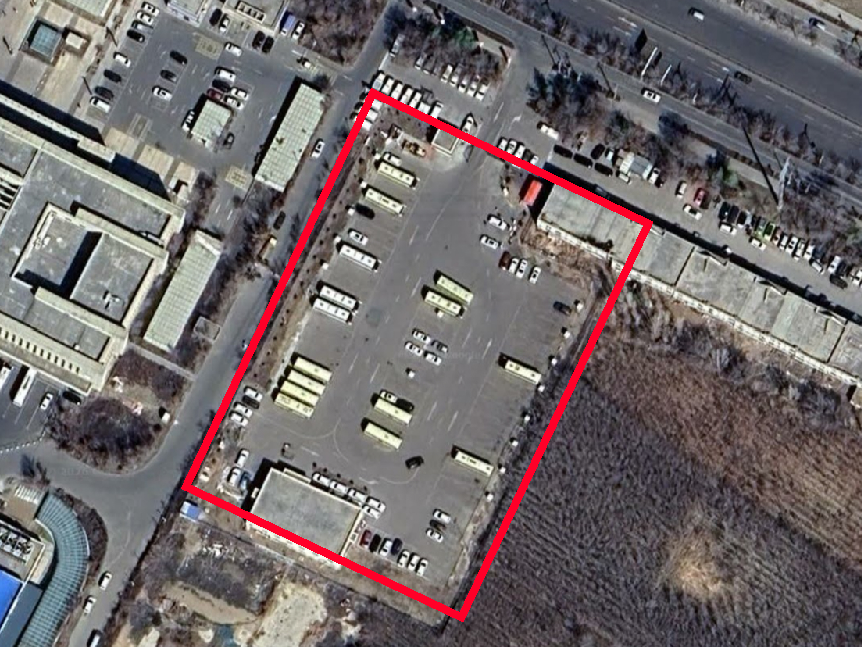
\includegraphics[height=4.2cm]{figures/GoogleMap_full}}\hfil
\subfloat[]{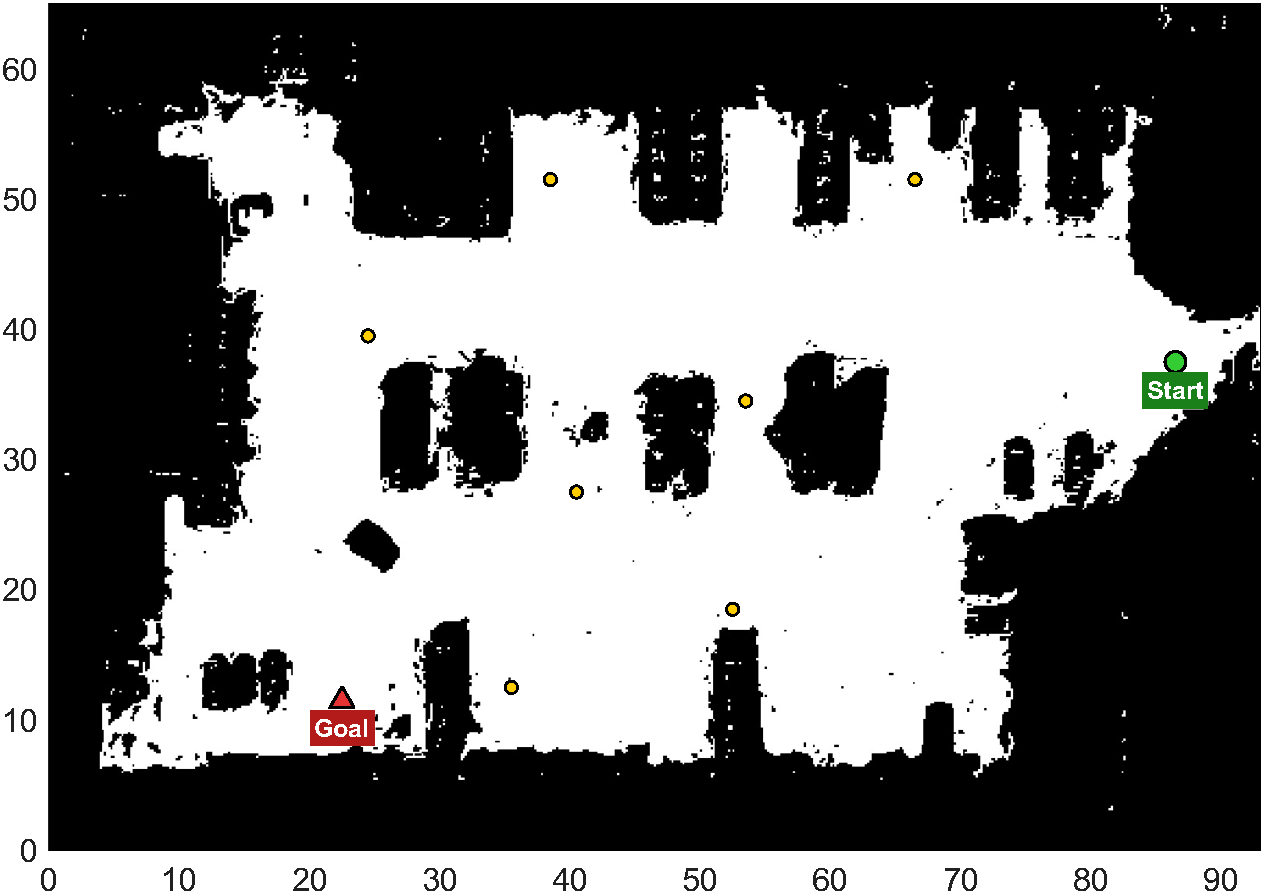
\includegraphics[height=4.2cm]{figures/GoogleMap_01goal}}\hfil
\subfloat[]{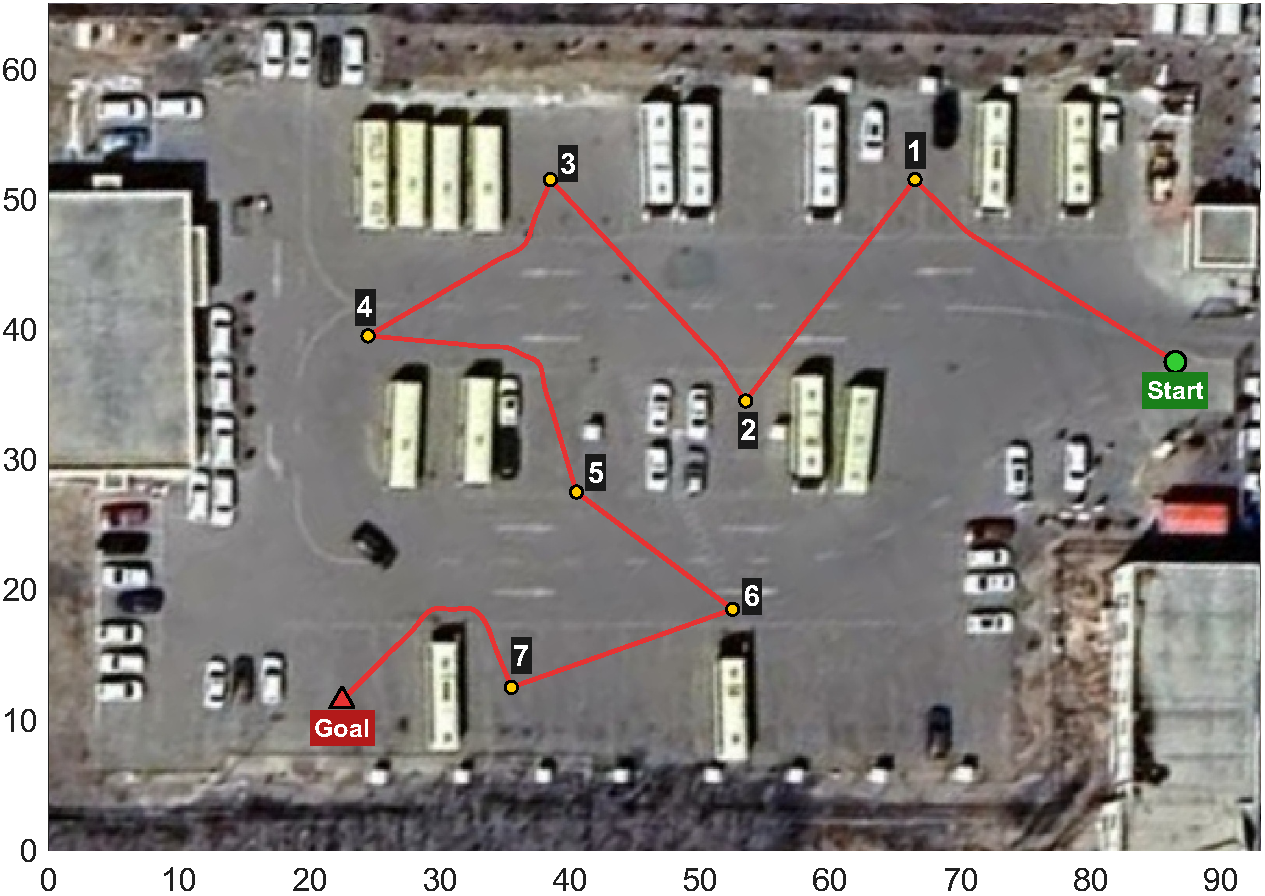
\includegraphics[height=4.2cm]{figures/GoogleMap_Path}}
\caption{Validation on a real satellite scene. (a) Region cropped from Google Maps, with the red box marking the experimental site; (b) the converted binary map and goal configuration; (c) the planned path overlaid on the real map background.}
\label{fig:googlemap}
\end{figure*}

\section{Conclusion}
\label{sec:concl}

This paper proposed a two-level planning framework for multi-goal traversal in static obstacle environments. Pairwise paths are obtained by a JPS-based improved A* search; safety-distance-aware path simplification and spline smoothing are used to construct an obstacle-constrained cost matrix from the processed continuous trajectories; and the MMAS-VND-CL solver then determines the goal visiting order. Experiments show that the improved A* achieves a planning time of 11.85 ms on Map~2, lower than conventional A* (29.19 ms) and Dijkstra (202.29 ms), and that the processed continuous trajectories are approximately 4.7\%--5.3\% shorter than the compared original grid paths. On the standard kroB100 closed-loop benchmark, MMAS-VND-CL reaches the known optimal tour cost of 22141 with a hit rate of 97.5\%, and a mean cost of 22142.45. Ablation results show that VND local search and the MMAS pheromone boundary play important roles in solution quality and stability. A grid map constructed from satellite imagery further demonstrates the method's ability to handle obstacle layouts in practical scenes.


\begin{thebibliography}{40}
\bibitem{ref1}

C.~Chen, J.~Frey, P.~Arm, and M.~Hutter, ``SMUG planner: A safe multi-goal planner for mobile robots in challenging environments,'' \textit{IEEE Robot. Autom. Lett.}, vol.~8, no.~11, pp.~7170--7177, 2023, doi: 10.1109/LRA.2023.3311207.


\bibitem{ref2}

T.~T.~C. Giang, H.~T.~T. Binh, H.~V.~D. Luong, N.~H. Hoang, and D.~Q. Huy, ``Fast marching firework method for multi-goal mobile robot path planning in complex obstacle maps,'' \textit{Intell. Service Robot.}, vol.~18, no.~6, pp.~1467--1484, 2025, doi: 10.1007/s11370-025-00654-6.


\bibitem{ref33}

K.~Karur, N.~Sharma, C.~Dharmatti, and J.~E. Siegel, ``A survey of path planning algorithms for mobile robots,'' \textit{Vehicles}, vol.~3, no.~3, pp.~448--468, 2021, doi: 10.3390/vehicles3030027.


\bibitem{ref37}

J.~Wang and M.~Q.-H. Meng, ``Real-time decision making and path planning for robotic autonomous luggage trolley collection at airports,'' \textit{IEEE Trans. Syst., Man, Cybern.: Syst.}, vol.~52, no.~4, pp.~2174--2183, 2022, doi: 10.1109/TSMC.2020.3048984.


\bibitem{ref38}

A.~Bolu and \"O.~Kor\c{c}ak, ``Adaptive task planning for multi-robot smart warehouse,'' \textit{IEEE Access}, vol.~9, pp.~27346--27358, 2021, doi: 10.1109/ACCESS.2021.3058190.


\bibitem{ref4}

S.~Saller, J.~Koehler, and A.~Karrenbauer, ``A survey on approximability of traveling salesman problems using the TSP-T3CO definition scheme,'' \textit{Ann. Oper. Res.}, vol.~351, no.~3, pp.~2129--2190, 2025, doi: 10.1007/s10479-025-06641-5.


\bibitem{ref36}

P.~C. Pop, O.~Cosma, C.~Sabo, and C.~Pop Sitar, ``A comprehensive survey on the generalized traveling salesman problem,'' \textit{Eur. J. Oper. Res.}, vol.~314, no.~3, pp.~819--835, 2023, doi: 10.1016/j.ejor.2023.07.022.


\bibitem{ref39}

J.~Faigl, ``On the performance of self-organizing maps for the non-Euclidean traveling salesman problem in the polygonal domain,'' \textit{Inf. Sci.}, vol.~181, no.~19, pp.~4214--4229, 2011, doi: 10.1016/j.ins.2011.05.019.


\bibitem{ref5}

P.~E. Hart, N.~J. Nilsson, and B. Raphael, ``A formal basis for the heuristic determination of minimum cost paths,'' \textit{IEEE Trans. Syst. Sci. Cybern.}, vol.~4, no.~2, pp.~100--107, 1968.


\bibitem{ref6}

E.~W. Dijkstra, ``A note on two problems in connexion with graphs,'' \textit{Numer. Math.}, vol.~1, no.~1, pp.~269--271, 1959.


\bibitem{ref7}

S.~M. LaValle, ``Rapidly-exploring random trees: A new tool for path planning,'' Dept. Comput. Sci., Iowa State Univ., Ames, IA, USA, Tech. Rep. 98-11, 1998.


\bibitem{ref34}

J.~A. Abdulsaheb and D.~J. Kadhim, ``Classical and heuristic approaches for mobile robot path planning: A survey,'' \textit{Robotics}, vol.~12, no.~4, p.~93, 2023, doi: 10.3390/robotics12040093.


\bibitem{ref35}

K.~Katona, H.~A. Neamah, and P.~K\"or\"ondi, ``Obstacle avoidance and path planning methods for autonomous navigation of mobile robot,'' \textit{Sensors}, vol.~24, no.~11, p.~3573, 2024, doi: 10.3390/s24113573.


\bibitem{ref8}

D.~T. Xuan, N.~T. Hung, and V.~T. Thang, ``A comprehensive review of improved A* path planning algorithms and their hybrid integrations,'' \textit{Automation}, vol.~6, no.~4, p.~52, 2025, doi: 10.3390/automation6040052.


\bibitem{ref10}

M. Likhachev, G. Gordon, and S. Thrun, ``ARA*: Anytime A* with provable bounds on sub-optimality,'' in \textit{Adv. Neural Inf. Process. Syst. (NIPS)}, 2003, pp.~767--774.


\bibitem{ref11}

D. Harabor and A. Grastien, ``Online graph pruning for pathfinding on grid maps,'' in \textit{Proc. 25th AAAI Conf. Artif. Intell. (AAAI-11)}, 2011, pp.~1114--1119.


\bibitem{ref12}

D. Harabor and A. Grastien, ``Improving jump point search,'' in \textit{Proc. 24th Int. Conf. Automated Planning Scheduling (ICAPS-14)}, 2014, pp.~128--135.


\bibitem{ref44}

D. Harabor and A. Grastien, ``The JPS pathfinding system,'' in \textit{Proc. Int. Symp. Comb. Search (SoCS)}, vol.~3, no.~1, pp.~207--208, 2021, doi: 10.1609/socs.v3i1.18254.


\bibitem{ref13}

C.~Gao, H.~Ding, D.~Zhang, and Y.~Wu, ``Improved JPS and DWA path planning algorithm for mobile robots,'' \textit{Mechatronics}, vol.~118, p.~103540, 2026, doi: 10.1016/j.mechatronics.2026.103540.


\bibitem{ref14}

R.~Guo, X.~Quan, and C.~Bao, ``Research on mobile robot path planning based on an improved bidirectional jump point search algorithm,'' \textit{Electronics}, vol.~14, no.~8, p.~1669, 2025, doi: 10.3390/electronics14081669.


\bibitem{ref15}

``Adaptive weight optimization based jump point Theta* algorithm in mobile robot path planning for intricate environments,'' \textit{Discover Appl. Sci.}, vol.~7, p.~11, 2025, doi: 10.1007/s42452-025-07932-z.


\bibitem{ref16}

I.~Munasinghe, A.~G. Perera, S.~Anavatti, and M.~Garratt, ``UGV path optimization in UAV-assisted environments using visibility-aware path simplification,'' \textit{J. Sens. Actuator Netw.}, vol.~15, no.~3, p.~41, 2026, doi: 10.3390/jsan15030041.


\bibitem{ref17}

J.~Ahmad and M.~N. Ab Wahab, ``Enhancing the safety and smoothness of path planning through an integration of Dijkstra's algorithm and piecewise cubic Bezier optimization,'' \textit{Expert Syst. Appl.}, vol.~289, p.~128315, 2025, doi: 10.1016/j.eswa.2025.128315.


\bibitem{ref18}

O.~E. Turan, O.~Misir, and M.~Ozden, ``Adaptive A*/NSGA-II framework for multi-goal navigation of mobile robots,'' \textit{Meas. Sci. Technol.}, 2026, doi: 10.1088/1361-6501/ae9209.


\bibitem{ref41}

F.~Huo, S.~Zhu, H.~Dong, and W.~Ren, ``A new approach to smooth path planning of Ackerman mobile robot based on improved ACO algorithm and B-spline curve,'' \textit{Robot. Auton. Syst.}, vol.~175, p.~104655, 2024, doi: 10.1016/j.robot.2024.104655.


\bibitem{ref19}

J.~H. Holland, \textit{Adaptation in Natural and Artificial Systems}. Ann Arbor, MI, USA: Univ. Michigan Press, 1975.


\bibitem{ref21}

M. Dorigo, V. Maniezzo, and A. Colorni, ``Ant system: Optimization by a colony of cooperating agents,'' \textit{IEEE Trans. Syst., Man, Cybern. B}, vol.~26, no.~1, pp.~29--41, 1996.


\bibitem{ref42}

Y.~Wang and Z.~Han, ``Ant colony optimization for traveling salesman problem based on parameters optimization,'' \textit{Appl. Soft Comput.}, vol.~107, p.~107439, 2021, doi: 10.1016/j.asoc.2021.107439.


\bibitem{ref22}

M. Dorigo and L.~M. Gambardella, ``Ant colony system: A cooperative learning approach to the traveling salesman problem,'' \textit{IEEE Trans. Evol. Comput.}, vol.~1, no.~1, pp.~53--66, 1997.


\bibitem{ref23}

T. St\"utzle and H.~H. Hoos, ``MAX--MIN ant system,'' \textit{Future Gener. Comput. Syst.}, vol.~16, no.~8, pp.~889--914, 2000.


\bibitem{ref24}

P. Hansen and N. Mladenovi\'c, ``Variable neighborhood search: Principles and applications,'' \textit{Eur. J. Oper. Res.}, vol.~130, no.~3, pp.~449--467, 2001.


\bibitem{ref25}

N.~A. Kyriakakis, M. Marinaki, and Y. Marinakis, ``A hybrid ant colony optimization--variable neighborhood descent approach for the cumulative capacitated vehicle routing problem,'' \textit{Comput. Oper. Res.}, vol.~134, p.~105397, 2021.


\bibitem{ref43}

X.~Zhou, H.~Ma, J.~Gu, H.~Chen, and W.~Deng, ``Parameter adaptation-based ant colony optimization with dynamic hybrid mechanism,'' \textit{Eng. Appl. Artif. Intell.}, vol.~114, p.~105139, 2022, doi: 10.1016/j.engappai.2022.105139.


\bibitem{ref26}

F.~Uddin, N.~Riaz, A.~Manan, I.~Mahmood, O.-Y. Song, A.~J. Malik, and A.~A. Abbasi, ``An improvement to the 2-opt heuristic algorithm for approximation of optimal TSP tour,'' \textit{Appl. Sci.}, vol.~13, no.~12, p.~7339, 2023, doi: 10.3390/app13127339.


\bibitem{ref27}

X.~Li, J.-Y. Li, C.~Chen, Z.-H. Zhan, S.~Kwong, and J.~Zhang, ``Matrix-based ant colony system for traveling salesman problem,'' in \textit{Proc. IEEE Int. Conf. Syst., Man, Cybern. (SMC)}, 2024, pp.~1358--1363, doi: 10.1109/SMC54092.2024.10831943.


\bibitem{ref28}

T.~Huang, Z.-Q. Zhang, Y.-J. Gong, and J.~Liu, ``nLKH-ACS: A niching Lin-Kernighan--Helsgaun-based ant colony system for multisolution traveling salesman problems,'' \textit{IEEE Trans. Evol. Comput.}, vol.~29, no.~6, pp.~2596--2610, 2024, doi: 10.1109/TEVC.2024.3507777.


\bibitem{ref29}

M.~Lin and L.~P. Schaposnik, ``A carbon aware ant colony system for the sustainable generalized traveling salesman problem,'' \textit{Sci. Rep.}, vol.~15, p.~21928, 2025, doi: 10.1038/s41598-025-08276-9.


\bibitem{ref30}

B.~Sun, W.-J. Yu, Z.-J. Wang, and J.-Y. Li, ``Ant colony optimization for multiple traveling salesmen problem with revisitable cities,'' in \textit{Proc. IEEE Int. Conf. Mach. Intell. Theory Appl. (MiTA)}, 2024, pp.~1--6, doi: 10.1109/MiTA60795.2024.10751693.


\bibitem{ref40}

B.~Behdani and J.~C. Smith, ``An integer-programming-based approach to the close-enough traveling salesman problem,'' \textit{INFORMS J. Comput.}, vol.~26, no.~3, pp.~415--432, 2014, doi: 10.1287/ijoc.2013.0574.


\bibitem{ref32}

B. Yao, C. Chen, X. Song, and X. Yang, ``Fresh seafood delivery routing problem using an improved ant colony optimization,'' \textit{Ann. Oper. Res.}, vol.~273, no.~1--2, pp.~163--186, 2019, doi: 10.1007/s10479-017-2531-2.

\end{thebibliography}

\end{document}


